\documentclass[12pt,letterpaper,english]{report}
\usepackage{setspace}
\setstretch{1.3}
\usepackage{bbm}
\usepackage{geometry} 
\geometry{letterpaper}
\usepackage[english]{babel}
% \usepackage[papersize={170mm,225mm},bmargin=20mm,lmargin=25mm,rmargin=20mm]{geometry}  % Para tamaño ITAM
\usepackage{graphicx}
\usepackage[utf8]{inputenc}
\usepackage{verbatim}  
\usepackage{enumerate}
\usepackage{fancyhdr} 
\usepackage{multicol}
\pagestyle{fancy} 
\usepackage{amsmath,amsfonts,amssymb,amsthm,epsfig,epstopdf,titling,url,array}
\usepackage{lscape}
\usepackage{float}
\usepackage{hyperref}
% \usepackage[colorlinks,citecolor={blue},urlcolor={blue}]{hyperref}
\usepackage[labelsep=period,hypcap]{caption}
\usepackage{subcaption} % \usepackage{subfig}
\usepackage{longtable}
\usepackage{tabularx}
\usepackage{filecontents,ltxtable}
\usepackage{multirow}
\usepackage{xcolor}
\usepackage{url}
\usepackage[]{titlesec}
\usepackage[export]{adjustbox}
\usepackage[title,titletoc]{appendix}

%%%%%%%%%%%%%%%%%%%%%%%%%%%%%%%%%%%%%%%%%%%%%%%%%%%%%%%%
%%%%%%%%%%%%% Biblio super chingona %%%%%%%%%%%%%%%%%%%%
%%%%%%%%%%%%%   carpetri@gmail.com  %%%%%%%%%%%%%%%%%%%%
%%%%%%%%%%%%%%%%%%%%%%%%%%%%%%%%%%%%%%%%%%%%%%%%%%%%%%%%
\usepackage{csquotes}
\usepackage[backend=bibtex,uniquename=false,firstinits=false,
            bibstyle=authoryear,
            citestyle=authoryear,
            url=true,
            sorting=nyt]{biblatex}

\renewcommand*{\nameyeardelim}{\addcomma\addspace}
\renewcommand*{\bibinitdelim}{}
\renewbibmacro{in:}{} 
\setlength\bibitemsep{1.5\itemsep}

\makeatletter

\newrobustcmd*{\parentexttrack}[1]{%
  \begingroup
  \blx@blxinit
  \blx@setsfcodes
  \blx@bibopenparen#1\blx@bibcloseparen
  \endgroup}

\AtEveryCite{
  \let\parentext=\parentexttrack
  \let\bibopenparen=\bibopenbracket
  \let\bibcloseparen=\bibclosebracket
  }

\AtEveryCitekey{\ifentrytype{misc}{\clearfield{labelyear}web page }{}}

\AtEveryBibitem{
  \ifentrytype{misc}{
  \DeclareNameFormat{last-first}{
  \iffirstinits
    {\usebibmacro{name:last-first}{#1}{#4}{#5}{#7}}
    {\usebibmacro{name:last-first}{#1}{#3}{#5}{#7}}
  \usebibmacro{name:andothers}}
  }{}
  }

\makeatother
\addbibresource{biblio.bib}
%%%%%%%%%%%%%%%%%%%%%%%%%%%%%%%%%%%%%%%%%%%%%%%%%%%%%%%%


% \addto\captionsspanish{\renewcommand{\figurename}{\it{Imagen}}}
% \addto\captionsspanish{\renewcommand{\tablename}{\it{Tabla}}}
% \addto\captionsspanish{\renewcommand\listfigurename{Índice de imágenes}}
% \addto\captionsspanish{\renewcommand\listtablename{Índice de tablas}}
% \addto\captionsspanish{\renewcommand{\captionfont}{\tt}}


%%%%%%%%%%%%%%%%%%%%%%%%%%%%%%%%%%%%%%%%%%%%%%%%%%%%%%%%
%%%%%%%%%%%%% Encabezados %%%%%%%%%%%%%%%%%%%%%%%%%%%%%%
%%%%%%%%%%%%%   carpetri@gmail.com  %%%%%%%%%%%%%%%%%%%%
%%%%%%%%%%%%%%%%%%%%%%%%%%%%%%%%%%%%%%%%%%%%%%%%%%%%%%%%

\renewcommand{\headrulewidth}{.5pt} 
\renewcommand{\footrulewidth}{.0pt}
\renewcommand{\chaptermark}[1]{\markright{#1}}
\renewcommand{\sectionmark}[1]{\markright{#1}}
\fancyhead[R]{\scshape ITAM}
\fancyhead[L]{\scshape \rightmark}

%%%%%%%%%%%%%%%%%%%%%%%%%%%%%%%%%%%%%%%%%%%%%%%%%%%%%%%%
%%%%%%%%%%%%%%%%%%%%%%%%%%%%%%%%%%%%%%%%%%%%%%%%%%%%%%%%
%%%%%%%%%%%%% Código %%%%%%%%%%%%%%%%%%%%%%%%%%%%%%
%%%%%%%%%%%%%   carpetri@gmail.com  %%%%%%%%%%%%%%%%%%%%
%%%%%%%%%%%%%%%%%%%%%%%%%%%%%%%%%%%%%%%%%%%%%%%%%%%%%%%%
\usepackage{listings}
% \lstset{
%   stringstyle=\ttfamily,
%   basicstyle=\small,
%   showstringspaces=false,
%   commentstyle=\color{red},
%   keywordstyle=\color{blue}
% }
\definecolor{codegreen}{rgb}{0,0.6,0}
\definecolor{codegray}{rgb}{0.5,0.5,0.5}
\definecolor{codepurple}{rgb}{0.58,0,0.82}
\definecolor{backcolour}{rgb}{0.97,0.97,0.97}
 
\lstdefinestyle{mystyle}{
    language=Python,
    backgroundcolor=\color{backcolour},   
    commentstyle=\color{codegreen},
    keywordstyle=\color{magenta},
    numberstyle=\tiny\color{codegray},
    stringstyle=\color{codepurple},
    basicstyle=\ttfamily\footnotesize,
    breakatwhitespace=true,         
    breaklines=true,                 
    captionpos=t,                    
    keepspaces=false,                 
    % numbers=left,                    
    % numbersep=5pt,                  
    showspaces=false,                
    showstringspaces=false,
    showtabs=false,                  
    tabsize=1
}
 
\lstset{style=mystyle}
\renewcommand\lstlistingname{\it{Code}}
\renewcommand\lstlistlistingname{\it{Code}}


%%%%%%%%%%%%%%%%%%%%%%%%%%%%%%%%%%%%%%%%%%%%%%%%%%%%%%%%


%%%%%%%%%%%%%%%%%%%%%%%%%%%%%%%%%%%%%%%%%%%%%%%%%%%%%%%%
%%%%%%%%%%%%% Capítulos %%%%%%%%%%%%%%%%%%%%%%%%%%%%%%
%%%%%%%%%%%%%   carpetri@gmail.com  %%%%%%%%%%%%%%%%%%%%
%%%%%%%%%%%%%%%%%%%%%%%%%%%%%%%%%%%%%%%%%%%%%%%%%%%%%%%%
\titleformat{\chapter} % command
[display] % shape
{\bfseries \LARGE} % format
{\rule{\textwidth}{0.9pt} Chapter \ \thechapter.} % label
{0.0ex} % sep
{   \centering } 
[
\vspace{-0.5ex}%
\rule{\textwidth}{0.9pt}
] % after-code
%%%%%%%%%%%%%%%%%%%%%%%%%%%%%%%%%%%%%%%%%%%%%%%%%%%%%%%%

\theoremstyle{plain}
\newtheorem{thm}{Theorem}[section]
\newtheorem{lem}[thm]{Lemma}
\newtheorem{prop}[thm]{Proposition}
\newtheorem*{cor}{Corollary}
\theoremstyle{definition}
\newtheorem{definition}{Definition}[section]
% \newtheorem{conjecture}{Conjecture}[section]
% \newtheorem{example}{Example}[section]
\theoremstyle{remark}
\newtheorem*{rem}{remark}
\newtheorem*{note}{note}

\title{Detecting Corruption Collusion and Fraud}
\author{Carlos Petricioli}


\begin{document}


% A. Preliminaries
\thispagestyle{empty}
\begin{center}
\LARGE \scshape Instituto Tecnológico Autónomo de México \\
\end{center}

\vspace{4mm}



\begin{center}

\includegraphics[scale=.7]{../img/ITAM.jpg}


\vspace{15mm}


\scshape \Large \thetitle
% \scshape \Large Detecting Corruption Collusion and Fraud

\vfill
\scshape \large T E S I S 


\vspace{3mm}
\scshape Que para obtener el título de \\

\vspace{3mm}
\scshape Maestro en Ciencia de Datos

\vspace{3mm}
\scshape Presenta

\vspace{4mm}
\Large CARLOS EDUARDO PETRICIOLI ARAIZA


\vspace{5mm}

\large Asesor: Dr.  Adolfo Javier De Unánue Tiscareño
\end{center}
\vspace{10mm}
México, D.F.   \hfill       2016


\newpage

\thispagestyle{empty}

\begin{flushright}
\textit{(This page is intentionally left blank)}
\end{flushright}

\newpage
\thispagestyle{plain}
\pagenumbering{Roman}
\setcounter{page}{1}

\noindent ``Con fundamento en los artículos 21 y 27 de la Ley Federal del Derecho de Autor y como titular de los derechos moral y patrimonial de la obra titulada `{\scshape XXXXX}' otorgo de manera gratuita y permanente al Instituto Tecnológico Autónomo de México y a la Biblioteca Raúl Baillères Jr., autorización para que fijen la obra en cualquier medio, incluido el electrónico y la divulguen entre sus usuarios, profesores, estudiantes o terceras personas, sin que pueda percibir por tal divulgación una contraprestación''.

\begin{center}

\bigskip

\bigskip

\bigskip

\scshape Carlos Eduardo Petricioli Araiza

\vfill

\makebox[3.5 in]{\hrulefill}

\bigskip

FECHA

\bigskip

\bigskip

\bigskip

\makebox[3.5 in]{\hrulefill}

\bigskip

FIRMA
\end{center}

\newpage

\thispagestyle{plain}


\begin{flushright}
\textit{Aquí van los agradecimientos}

\end{flushright}

\newpage

\thispagestyle{plain}



\begin{flushright}
\textit{Aquí va la dedicatoria}

\end{flushright}


\tableofcontents
\thispagestyle{plain}

\listoffigures
\thispagestyle{plain}

\listoftables
\newpage


% !TEX root = A0_thesis_detecting_collusion_corruption_fraud.tex
\thispagestyle{plain}
\pagenumbering{arabic}
\begin{center}
% \scshape \large Detecting Corruption Collusion and Fraud\footnote{ Last Update: \today.}
\scshape \normalsize Cómo identificar corrupción, colusión y fraude en los contratos que otorga el Banco Mundial
% Tesis de Licenciatura para obtener el grado de Licenciado en Matemáticas Aplicadas por el Instituto Tecnológico Autónomo de México (ITAM). México D.F., 2015.  \\}
\bigskip

\scshape \normalsize \theauthor\footnote{ \tiny Agradezco al Dr. Rayid Ghani  y al  Dr.  Eric Rozier por su asesoría en la elaboración de este trabajo. También agradezco la colaboración y los comentarios del Dr. Jeff Alstott, Mtro. Dylan Fitzpatrick, y Dr. Misha Teplitskiy y de Elizabeth Wiramidjaja.
\\  \href{mailto:carpetri@gmail.com}{\texttt{carpetri@gmail.com}}  \hfill \href{http://detecting-corruption.carlospetricioli.com}{\texttt{detecting-corruption.carlospetricioli.com}} }
\normalsize
\end{center}

\section*{\centering  \normalsize{Resumen} }
% \begin{quotation}
% \scriptsize
\footnotesize
% \noindent 


Para combatir la pobreza mundial, El Banco Mundial presta billones de dólares  para financiar proyectos de desarrollo social. Este trabajo pretende ayudar a los investigadores del Banco Mundial a buscar e identificar patrones que indiquen posible corrupción, colusión y fraude en los datos de los contratos que otorga por medio del uso de modelos por contrato que estiman el riesgo que tienen de ser este tipo de casos. Este trabajo tiene potencial para aportar en la capacidad que tiene el Banco Mundial para detectar este tipo de ofensas, al menos priorizando las investigaciones futuras.

El problema es que  los proveedores que ofrecen bienes y servicios en los proyectos suelen estar seleccionados por medio de un proceso  de subastas/licitaciones que en la práctica deberían ser abiertas y competitivas pero que en la realidad no lo son del todo. Los contratistas manipulan el proceso competitivo coludiéndose con otros contratistas y ofreciendo sobornos a miembros del gobierno, entre otras ofensas. Este tipo de ofensas tienen consecuencias importantes en los precios y en la calidad de entrega de los contratos y proyectos. En este trabajo se desarrollan modelos por contrato para identificar el riesgo que presentan de tener este tipo de ofensas con base en datos históricos de contratos otorgados en los últimos 20 años y en datos de investigaciones que ha realizado el Banco Mundial anteriormente incluyendo empresas y proyectos que se investigaron. 

Para esto, se creó una aplicación que les permite a los investigadores dentro del Banco Mundial, seguir el desarrollo de una empresa en específico a lo largo de distintos países, sectores y en el tiempo. Por medio de esta herramienta, los investigadores del Banco Mundial pueden tener mejor control sobre los contratos que cada empresa ha recibido, así como los distintos nombres con los cuales se ha registrado en las distintas bases de datos y todo además con  un indicador del nivel de riesgo para cada uno de los contratistas del Banco Mundial con base en variables que incluyen, entre otras, datos de la red de empresas/proyectos. La aplicación también incluye visualizaciones de lo anterior.

En conclusión, los datos con los que cuenta actualmente el Banco Mundial son suficientes para identificar el riesgo de corrupción, colusión y fraude y permite que el Banco Mundial investigue de una manera proactiva para determinar qué empresas, proyectos o contratos analizar.


\thispagestyle{plain}
\vfill
\scriptsize \noindent \textbf{Palabras clave:} Corrupción, Colusión, Fraude, Banco Mundial.
\normalsize
% !TEX root = A0_thesis_detecting_collusion_corruption_fraud.tex
\newpage
\thispagestyle{plain}
\pagenumbering{arabic}
\begin{center}
\scshape \large Detecting Corruption Collusion and Fraud\footnote{ Last Update: \today.}
% \scshape \large \thetitle\footnote{  Last Update: \today.}
% Tesis de Licenciatura para obtener el grado de Licenciado en Matemáticas Aplicadas por el Instituto Tecnológico Autónomo de México (ITAM). México D.F., 2015.  \\}
\\

\scshape \theauthor\footnote{ I especially thank Rayid Ghani (Ph.D. Carnegie Mellon University) and  Eric Rozier (Ph.D. University of Illinois Urbana-Champaign) for their mentorship throughout the elaboration of this work. I also appreciate the collaboration and comments of Jeff Alstott (Ph.D. Cambridge), Dylan Fitzpatrick (Ph.D. Carnegie Mellon), Misha Teplitskiy (Ph.D. University of Chicago) and Elizabeth Wiramidjaja (World Bank).
\\  \href{mailto:carpetri@gmail.com}{\texttt{carpetri@gmail.com}}  \hfill \href{http://detecting-corruption.carlospetricioli.com}{\texttt{detecting-corruption.carlospetricioli.com}} }
\normalsize
\end{center}

\section*{\centering  \normalsize{Abstract} }
% \begin{quotation}

\small
\noindent The World Bank Group lends billions of dollars each year to fund development projects in its efforts to reduce global poverty. This project helps investigators at the Bank search for patterns of collusion, corruption, and fraud in its contracts data by using models of contract-specific risk. An automated approach like this can  highly increase the World Bank's ability to detect these offenses by efficiently targeting  their future investigations. 

The actual problem is that contractors providing goods and services on World Bank's projects are typically hired through a competitive bidding process, but occasionally, prospective contractors influence the competitive system by colluding with other contractors, bribing government officials, or otherwise manipulating the bidding process. These offenses have far-reaching effects on the price and quality of contract delivery. This project develops contract-level risk models that use historical data on major contracts awarded from the past 20 years and internal investigations data, covering companies and projects investigated  in the past.

To approach the problem,  an interactive dashboard was developed for investigators to track any company's activity across countries, sectors, and time. By using this tool, investigators can track contract awards companies have received, including under different names, view a risk score for each World Bank contract, as calculated by our contract risk model and visualize the immediate neighborhood of the company in its co-award network.

In conclusion, current data is sufficient to forecast risk and allows  investigators to be proactive in determining which companies, projects and contracts to examine.
% \end{quotation}
\thispagestyle{plain}
\vfill
\scriptsize \noindent \textbf{Keywords:} Machine Learning, Corruption, Fraud, The World Bank.
\normalsize


% !TEX root = A0_thesis_detecting_collusion_corruption_fraud.tex
\chapter*{Web page}

% \noindent Para la divulgación, presentación y retroalimentación sobre este trabajo se creó la página indicada a continuación en donde se puede encontrar una copia de este trabajo así como materiales adicionales.

\begin{center}
\Large{\href{http://detecting-corruption.carlospetricioli.com}{detecting-corruption.carlospetricioli.com}}
\end{center}
\normalsize

% Como resultado de este trabajo y con el fin de promover la investigación y el desarrollo de métodos estadísticos y econométricos que utilicen alternativas innovadoras para generar mejores estimaciones  de las cuentas nacionales a niveles más desagregados de lo que se puede encontrar en las cuentas nacionales de México actualmente, en la página se incluyen  todos los datos  procesados de la serie de tiempo de imágenes satelitales desde 1992 hasta 2013 identificados por pixel con coordenadas geográficas de longitud y latitud identificadas con todos los Estados, Municipios y AGEBs urbanos de México. Además, se incluye el valor de la calibración que se realizó en este trabajo para hacer comprable intertemporalmente esta serie de tiempo de iluminación  nocturna  visible desde el espacio.
\newpage


%  \thispagestyle{empty}
%  
% \begin{flushright}
% \textit{(Esta página está en blanco)}
% \end{flushright}
% 
% \newpage
\thispagestyle{plain}

% B. Chapters
% !TEX root = A0_thesis_detecting_collusion_corruption_fraud.tex
\chapter{Introduction}\label{chap_intro}

This project was made at the Eric \& Wendy Schmidt, Data Science for Social Good (DSSG) summer fellowship at the University of Chicago during the summer of 2014. As a data fellow I was assigned to the the project of Detecting Corruption, Collusion and Fraud with the World Bank as a partner.  My mentor was Eric Rozier from the University of Cincinnati, my teammates were Dylan Fitzpatick, Jeff Alstott and Misha Teplitskiy, our partner from the World Bank was  Elizabeth Wiramidjaja and we all worked under the supervision of Rayid Ghani, the director of the DSSG. This paper is a report of what was made during the elaboration of that project. Some of the visualizations and data was private so this paper shows the public version of this project. For some visualizations and interpretations, fake data was used to protect the confidentiality.

The World Bank Group lends billions of dollars each year to fund development projects in its effort to reduce global poverty. This project helps investigators at the Bank to search for patterns of collusion, corruption, and fraud in its contracts data, by using models of contract-specific risk. By developing an automated approach to detect these offenses this project can help the World Bank efficiently target future investigations.

Several things are required for a project of this type to achieve success. The following list outlines the requirements for a successful project. Some requirements easier to satisfy so it is ordered from  the easiest to the most difficult. These alone do not guarantee success, but success is nearly impossible without them \parencite{dssg_proj_list}\label{dssg}.   \textit{1. A solvable problem}. This project cannot solve poverty, but it can help alleviate it by reducing corruption, collusion and fraud. 
\textit{2. A challenging problem}. Challenging problems encourage teamwork, spawn creative solutions, and play a key role in a Data Scientist's ability to solve real-world problems and provide understanding, excitement, and passion for solving problems with social impact. For example, this World Bank project involved  search-engine expertise to find links between corrupt applicants online. 
\textit{3. An important problem with social impact}. Working in a big project is an investment, not only financially, but also opportunistically (when someone choose to do a project, someone is choosing not to do another). It is important to dedicate the limited resources to substantial problems. Each project must meet an operational need for the partner organization and must have a tangible connection to ``social good.'' For example, this project helps more people over fewer people and that solve chronic problems over temporary problems. 
\textit{4. A motivated, capable, and committed partner}. No project can succeed without a fully invested project partner. Project partners understand the problem, they have subject-matter expertise, and they ultimately decide how a Data Scientist's work is used. Partners often look at the problem differently, which is important for solving tough problems.  Partners provide insight into the problem and guide Data Scientists to develop a solution. This demands a lot from partners. It often requires partners stretching themselves and asking themselves hard questions. It also requires time. For this project, the World Bank helped scope the problem before it started, they gave a complete presentation about their work, they were available for at least once a week for feedback and discussion during the duration of the project, and they are actually using the results of this work when it finished. 
\textit{5. Appropriate, relevant data}. Getting the data a project  needs is almost always the biggest challenge. Important things go unmeasured or unrecorded or, more commonly, cannot be shared. Many projects involve  sensitive information. Getting lawyers to agree on data and code sharing can take months. It is important for Data Scientists to be flexible. Partners have anonymized data (while keeping it useful at an individual level), conducted background checks, and require Data Scientists to do analyses on their internal computer systems (remotely). All this while maintaining a spirit of openness.  In this case, the World Bank contributed with all the relevant data they have in order to build a solution that's appropriate, effective, and easily deployed.

\section{The World Bank}\label{sec_intro_wb}

The World Bank was created in 1944 as one institution and has evolved into an association of five development institutions. It is composed by  the International Bank for Reconstruction and Development (IBRD), the International Development Association (IDA), the International Finance Corporation (IFC), the Multilateral Guarantee Agency (MIGA), and the International Center for the Settlement of Investment Disputes (ICSID). In its interior it was formed by a large group of engineers and financial analysts who work from Washington, D.C. Now, they have a very heterogeneous and distinct staff that includes economists, public policy experts, sector experts and social scientists and about one third of the workers have spread to the country offices. They have more than 10,000 employees in more than 120 offices worldwide. While reconstruction remains an important part of their objectives, however, at today's World Bank, poverty reduction through an inclusive and sustainable globalization remains the overarching goal. For details see \parencite{wb_history}. 

The World Bank Group has set three goals for the world to achieve by 2030; first, end extreme poverty by decreasing the percentage of people living on less than \$1.90 a day to no more than 3\%; second, promote shared prosperity by fostering the income growth of the bottom 40\% for every country; third, the World Bank is a vital source of financial and technical assistance to developing countries around the world. The World Bank Group is not a bank in the ordinary sense but a unique partnership to reduce poverty and support development \parencite{wb_about}.

The World Bank Group provides Financial Products and Services by giving out low-interest loans, zero to low-interest credits, and grants to developing countries.
\begin{quote} ``These support a wide array of investments in such areas as education, health, public administration, infrastructure, financial and private sector development, agriculture, and environmental and natural resource management. Some of our projects are cofinanced with governments, other multilateral institutions, commercial banks, export credit agencies, and private sector investors.''\parencite{wb_about}. \end{quote}They offer financing through trust fund partnerships with bilateral and multilateral donors. For example, many partners have asked the Bank to help manage initiatives that address needs across a wide range of sectors and developing regions. Projects vary widely in scale and scope, ranging from developing hydropower systems\footnote{ WASHINGTON, March 20, 2014–Sub-Saharan Africa is blessed with large hydropower resources that can bring electricity to homes, power businesses and industry, light clinics and schools, and spur economic activity, creating jobs and improving human well-being.  Yet, only 10\% of this hydropower potential has been mobilized, weakening the fight to end poverty and boost shared prosperity on the continent. See \cite{wb_hydro}} to rehabilitating coral reefs\footnote{ Wakatobi, Indonesia, June 5, 2014 - As the world's largest archipelago, Indonesia is blessed with at least 5.1 million hectares of coral reefs. However, almost 65 percent of the reefs are now considered threatened from overfishing. Almost half are considered threatened specifically from destructive fishing practices. Nadjib Prasyad runs the Fisheries Office in Wakatobi, South-east Sulawesi, and he laments the various activities that destroy the reefs and consequently threaten the livelihood of the villages: fish bombing, sand extraction, collection of the reefs themselves. Prasyad says that, once the reefs die, so do the fish: “We have nothing except our coral reefs.So we have to really protect them since they're the only source of our region's development. See \cite{wb_coral}} to improving roads, health, education and agriculture systems\footnote{ ``We didn't use to have bus service to the communities; now we have it every hour.'' ``Now we have a paved highway and signs; it's comfortable for traveling.'' ``When there was a drought, there was no water for the animals, for the pasture, for irrigating the produce we consumed and much less for crops for sale.'' ``With the water, people returned to the community and it is improving their quality of life.'' Today, these are some of the phrases that can be heard on the roads of Chimborazo, one of the largest provinces in Ecuador’s central highlands. See \cite{wb_roads} }.

This work focuses in these Financial Products and Services. It analyzes their contracts (see the chapter \ref{chap_procurements} for more details) by using historical data on over 300,000 major contracts funded by World Bank in the form of low-interest loans, zero to low-interest credits, and grants to developing countries covering  from the past 20 years. Historical data including such features as company name, country, sector, and total award amount.

The World Bank also provides Innovative Knowledge Sharing, by offering support to developing countries through policy advice, research and analysis, and technical assistance. \begin{quote}
``The analytical work often underpins World Bank financing and helps inform developing countries' own investments. In addition, we support capacity development in the countries we serve. We also sponsor, host, or participate in many conferences and forums on issues of development, often in collaboration with partners''\parencite{wb_about}.
\end{quote}

This is why this project becomes of high value for the World Bank Group. On one hand, this work helps them to provide much better Financial Products and Services by reducing the cost that corruption, collusion and fraud generates in the process of lending money to developing countries throughout the World's Development Banks. On the other, this project contributes to their Innovative Knowledge Sharing by supplying them with the necessary tools and algorithms they need in order to share corruption, collusion and fraud analysis' results.

This project relies on the fact that the World Bank group, in order to ensure that countries can access the best global expertise and help generate cutting-edge knowledge, is constantly seeking to improve the way it shares its knowledge and engages with clients and the public at large. This includes  measurable results, improving every aspect of their work like how projects are designed, how information is made available, and how to bring our operations closer to client governments and communities and also includes  their Open Development, a set of free, easy-to-access tools, research and knowledge to help people address the world's development challenges. This work would not be possible without all this previous work and is a virtuous circle because it contributes by helping them achieve this goal.

This work uses the Open Data\footnote{Go to \cite{wb_data}} website from the World Bank, which offers free access to comprehensive, downloadable indicators about development in countries around the globe, data needed in order to detect and predict patterns of collusion, corruption, and fraud in its contracts data by using models of contract-specific risk. 

To summarize, chapter \ref{chap_procurements} presents the way a procurement process is done. It presents all the details that an entity should fill in order to participate in a procurement process and it presents the legal definition of corruption, collusion, fraud and other offenses that could be made in the lending process. Also, it presents how the World Bank tags the entities that have been debarred and the reasons this might be. It describes how they investigate cases of corruption and other offenses to the World Bank along with possible indicators form the data that might indicate patterns of corruption, collusion and fraud.

After that, chapter \ref{chap_data} presents all the different data sources available for this project. It includes all the public and private data and it explains how to obtain the data form their original sources. This chapter also explains some modifications made to the data in order to have a better insight and the algorithms used to create features as well as the co-awards network for each entity in the data.

Then, chapter \ref{chap_product} describes the data product created for the World Bank to investigate their contractors and projects in a proactive way. It describes the modeling process as well as the details that the web dashboard includes created for the World Bank to perform investigations.

Finally, chapter \ref{chap_conclusion} presents the main conclusions of this project as well as the future work to be done.






% !TEX root = A0_thesis_detecting_collusion_corruption_fraud.tex
\chapter{The World Bank's Procurements}\label{chap_procurements}

As shown in the chapter \ref{chap_intro}, The World Bank Group provides Financial Products and Services by giving out low-interest loans, zero to low-interest credits, and grants to developing countries. They offer financing through trust fund partnerships with bilateral and multilateral donors.  This work focuses in these Financial Products and Services. It analyzes their contracts by using historical data on over 300,000 major contracts funded by World Bank.


\section{The World Bank Group's Rules and Guidelines}

The process by which the World Bank Group gives out low-interest loans, zero to low-interest credits, and grants to developing countries is not simple. They have a set of guidelines, available online \parencite{wb_g_proc}, in which they specify how to apply to all the contracts for goods, works and services financed in whole or in part from the Bank's loans, credits and grants which would thereby cover both International Bank for Reconstruction and Development (IBRD) and the International Development Association (IDA). Similar provisions apply for the selection of Consultants under the Consultants Guidelines \parencite{wb_g_cons}. For the purpose of this project the Consultants will not be deeply explained. 

In the World Bank's rules and guidelines they consider ``goods'' and ``works'' all the related services such as transportation, insurance, installation, commissioning, training, and initial maintenance. Also,  ``goods'' includes commodities, raw material, machinery, equipment, vehicles, and industrial plant. 

\begin{quote}
``This requirement is made applicable in each operation through the loan, credit or grant agreement thus making their use a legal obligation on the part of the Borrower. It applies as well to counterpart funds that are also used to finance contracts with loan/credit proceeds. In addition, parts of Bank-financed projects that are co-financed by other donors are also subject to Bank rules. This could also be the case under parallel financing when co-financiers agree to using Bank guidelines (leverage effect).''\parencite{wb_rules}
\end{quote}

In order to ensure that these legal provisions are observed during project implementation, the World Bank's staff reviews and provides a ``no objection'' before the Borrower implements certain procurement decisions\footnote{For all International Competitive Bidding (ICB) and other high-value, high-risk, and otherwise complex contracts}. Bank staff will review all the contracts that have not been subject to Prior Review so as to ensure that the Guidelines were applied as required. Where this is found not to be the case, the Bank applies various remedies including \textit{mis-procurement}, which in most instances requires cancellation and refund of the funds in question\footnote{Advertising requirements vary depending on whether Procurement is subject to International Competitive Bidding (ICB) or National Competitive Bidding(NCB).}.


\subsection{Procurements General Considerations}

In every Procurement the World Bank expects that the responsibility for the implementation of the project, and therefore for the award and administration of contracts under the project, rests with the Borrower. The Bank, is required ensure that the proceeds of any loan are used only for the purposes for which the loan was granted, with due attention to considerations of economy and efficiency and without regard to political or other non-economic influences or considerations. While in practice the specific procurement rules and procedures to be followed in the implementation of a project depend on the circumstances of the particular case, four considerations generally guide the Bank's requirements:
\begin{enumerate}[a)]
\item ``the need for economy and efficiency in the implementation of the project, including the procurement of the goods, works, and non-consulting services involved;
\item the Bank's interest in giving all eligible bidders from developed and developing countries the same information and equal opportunity to compete in providing goods, works, and non-consulting services financed by the Bank;
\item  the Bank's interest in encouraging the development of domestic contracting and manufacturing industries in the Borrowing country; and
\item the importance of transparency in the procurement process.''\footnote{See \cite{wb_g_proc}.}
\end{enumerate}


\subsection{Procurement Plan}

Any firm or person interested in a procurement has to submit a Procurement plan to the World Bank in which they specify general characteristics of the project such as the Bank’s approval date of the procurement plan, the date of general procurement notice and the period covered by the procurement plan. It has to include the details concerning the goods and works and non-consulting services required for the project such as the Prior Review Threshold, prequalification,  proposed procedures for CDD components, reference to (if any) project operational/procurement manual, any other special procurement arrangements, and a summary of the procurement packages planned during the first 18 months after project effectiveness. With regard to the consultants, it has to include a prior review threshold, short list comprising entirely of national consultants, any other special selection Arrangements (including advance procurement and retroactive financing, if applicable or delete if not applicable), and consultancy assignments with selection methods and time Schedule. The appendix \ref{app_proc_plan} shows a sample procurement plan to be filled \parencite{wb_sample_proc}. 


The World Bank's guidelines for procurement of goods, works, and non-consulting services \parencite{wb_g_proc} establishes that open competition is the basis for efficient public procurement.  In their articles, they state that each Borrower shall select the most appropriate method for the specific procurement. They have to choose between International Competitive Bidding (ICB) or National Competitive Bidding (NCB). This means, in most cases, ICB, properly administered, and with the allowance for preferences for domestically manufactured goods and, where appropriate, for domestic contractors for works under prescribed conditions is the most appropriate method. The Bank requires its Borrowers to obtain goods, works, and non-consulting services through ICB open to eligible suppliers, service providers, and contractors\footnote{Section II of these Guidelines describes the procedures for ICB \parencite{wb_g_proc}.}.

In order to satisfy these requirements, any procurement needs to be transparent, competitive and legal according to the guidelines the World Bank established. Contractors providing goods and services on World Bank projects are typically hired through a competitive bidding process. The problem is that in practice, the Borrowers and Contractors tend not to fulfill those requirements. Occasionally, prospective contractors influence the competitive system by colluding with other contractors, bribing government officials, or otherwise manipulating the bidding process. These offenses have far-reaching effects on the price and quality of contract delivery.  There is a considerable amount of cases in which corruption, collusion and/or fraud takes place. The guidelines include some sections to address those problems. The World Bank is committed to detecting instances of collusion, corruption, and fraud in order to maximize its global impact.

\section{Corruption, Collusion and Fraud}\label{sec_intro_corruption}

The World Bank's guidelines for procurement of goods, works, and non-consulting services \parencite{wb_g_proc} establishes what's to be understood by corruption, collusion, fraud, coercion and obstruction. 

It is the Bank's policy to require that Borrowers\footnote{including beneficiaries of Bank loans.}, bidders, suppliers, contractors and their agents\footnote{whether declared or not.}, sub-contractors, sub-consultants, service providers or suppliers, and any personnel thereof, observe the highest standard of ethics during the procurement and execution of Bank-financed contracts. In pursuance of this policy, the Bank defines, the terms set forth below as follows\footnote{Definitions taken from \cite{wb_g_proc}. Updated to 2011.}:

\begin{definition}\label{def_corruption}
A \textit{corrupt practice} is the offering, giving, receiving, or soliciting, directly or indirectly, of anything of value to influence improperly the actions of another party.
\end{definition}

\begin{definition}\label{def_collusion}
A \textit{collusive practice} is an arrangement between two or more parties designed to achieve an improper purpose, including to influence improperly the actions of another party.
\end{definition}

\begin{definition}\label{def_fraud}
A \textit{fraudulent practice} is any act or omission, including a misrepresentation, that knowingly or recklessly misleads, or attempts to mislead, a party to obtain a financial or other benefit or to avoid an obligation.
\end{definition}

\begin{definition}\label{def_coersion}
A \textit{coercive practice} is impairing or harming, or threatening to impair or harm, directly or indirectly, any party or the property of the party to influence improperly the actions of a party.
\end{definition}

\begin{definition}\label{def_obstruction}
A \textit{obstructive practice} is deliberately destroying, falsifying, altering, or concealing of evidence material to the investigation or making false statements to investigators in order to materially impede a Bank investigation into allegations of a corrupt, fraudulent, coercive or collusive practice; and/or threatening, harassing or intimidating any party to prevent it from disclosing its knowledge of matters relevant to the investigation or from pursuing the investigation, or acts intended to materially impede the exercise of the Bank's inspection and audit rights.
\end{definition}

In its effort to avoid practices from definitions \ref{def_collusion} to \ref{def_obstruction}, the World Bank
will respond accordingly to each contract in question. 
The Bank will \textit{reject a proposal} for award if it determines that the bidder recommended for award, or any of its personnel has, directly or indirectly, engaged in corrupt, fraudulent, collusive, coercive, or obstructive practices in competing for the contract in question. 
The Bank will \textit{declare mis-procurement} and cancel the loan if it determines at any time that representatives of the Borrower engaged in  any corrupt, fraudulent, collusive, coercive, or obstructive practices during the procurement or the implementation of the contract. 
The Bank will \textit{sanction} a firm or individual, including by publicly declaring such firm or individual ineligible, either indefinitely or for a stated period of time to be awarded a Bank-financed contract; and to be a nominated sub-contractor of an otherwise eligible firm being awarded a Bank-financed contract.
The Bank will require that a clause be included to permit the Bank to inspect all accounts, records, and other documents relating to the submission of bids and contract performance, and to have them audited by auditors appointed by the Bank.

\subsection{Examples: What is Fraud and Corruption?}

An example of fraud according to the definition \ref{def_fraud}: \begin{quote}
``In a few years since its establishment, a consulting company is awarded multiple World Bank Group-financed contracts totaling in millions of dollars.  The proposals submitted by the consulting company contain numerous past project experiences and references that contribute to its success and eligibility.  However, a review of the consulting company's past project experiences reveal that the company has claimed the experiences of individual consultants as its own, as well as grossly exaggerated the value of the projects that it has undertaken.  Not only is the consulting company misrepresenting its qualifications and capacity, it is also cutting its subconsultants' contracts by half, but claiming the full amount on its invoices to the client.  The quality of the deliverables from this consulting company is highly questionable, which affects the project's overall developmental goals.''\parencite{wb_examples}
\end{quote}

An example of corruption according to the definition \ref{def_corruption}: \begin{quote}
``A supplier agrees to pay kickbacks to a senior government official through an agent it hires as a sub-consultant to perform business development and marketing services but without any deliverables.  This agent is connected to a senior government official who is demanding a commission from every bidder as the official has influence over the bid evaluation committee and can steer the award of the contract to any bidder willing to pay.  This supplier builds in the kickback amount as a percentage of the contract value, and pays for it from the funds it receives from the World Bank Group-financed project. Project financing costs are artificially inflated by these practices, and the supplier recovers costs by providing less expensive and lower quality goods.''\parencite{wb_examples}
\end{quote}

% Collusion
An example of collusion according to the definition \ref{def_collusion}: \begin{quote}
``A project official arranges to steer contracts on a World Bank Group-financed project to his own company and that of his relatives.  The project official not only tells his relatives' companies what prices to put in their bids, but also what particular technical specification to include.  The bids of companies that are not part of this inner circle are disqualified as being technically non-responsive, leaving the project official's and his relatives' companies as the lowest evaluated bidders on the different contracts.  Not only is the integrity of the procurement process compromised, but the winning bid prices are considerably higher than what would have been with genuine competitive bidding.''\parencite{wb_examples}
\end{quote}

% Coercion
An example of coercion according to the definition \ref{def_coersion}: \begin{quote}
``A contractor is stopped from submitting his bid at the bid opening.  Persons connected to a competitor block the contractor from entering the building where the bid opening is taking place, and tell him that `if he cares for his family, he should not submit a bid.'  Another bidder who comes to submit a bid is also stopped by these same persons who tells the bidder that `it is not his turn to win this contract.'  The two bidders leave the bid opening and do not submit a bid out of fear.''\parencite{wb_examples}
\end{quote}

% Obstruction

An example of coercion according to the definition \ref{def_coersion}: \begin{quote}
``World Bank Group investigators contact a company alleged to have paid a bribe on a World Bank Group-financed contract and request to audit the company's financial records.  The company refuses to do so despite its agreement and obligation under the contract to allow the World Bank Group access to these records.  Furthermore, it withholds key documents and alters other documents that are given to the investigators.''\parencite{wb_examples}
\end{quote}


\section{World Bank Listing of Ineligible Contractors}

The World Bank has a long history of giving loans for procurement of goods, works, and non-consulting services based on the four considerations listed above. As expected, there has been a long history of malicious activity in the procurement process. This is why The World Bank publishes a list of contractors which had been discovered to have a practice that lead to either a rejection, a mis-procurement, an obstructive practice or a sanction. This project refers to this list as the debarment data.

The World Bank publishes an online \parencite{wb_debarment} list that includes all the firms and individuals listed as ineligible to be awarded a World Bank-financed contract for the periods indicated because they have been sanctioned under the Bank's fraud and corruption policy as set in the Procurement Guidelines or the Consultant Guidelines.  Such sanction was imposed as the result of an administrative process conducted by the Bank that permitted the accused firms and individuals to respond to the allegations\footnote{``Through July 2007, this process was conducted in accordance with the Sanctions Committee Procedures adopted on August 2, 2001. Since then, the process has been conducted in accordance with the Sanctions Procedures of the World Bank Group Sanctions Board.''}, or a cross-debarment\footnote{ Since 2011.} made effective by the World Bank, Asian Development Bank, European Bank for Reconstruction and Development, Inter-American Development Bank, and African Development Bank.

The table \ref{tab_debarred_sam} bellow shows a short sample of how is the debarments list published. As it can be seen from the table \ref{tab_debarred_sam}, it includes a \textit{Firm Name, Address, Country, Ineligibility Period} and \textit{Grounds}. The \textit{Firm Name} can be a person or an entity, the \textit{Ineligibility period} corresponds to the time frame in which that specific \textit{Firm Name} is debarred from receiving any type of award financed by the World Bank, and finally, the \textit{Grounds} refers to the violations made to the Consultants Guidelines (CG) or the Procurements Guidelines (PG) and their specific article and section.

\begin{table}[H]
\caption{Debarred Firms and Individuals (sample)}
\label{tab_debarred_sam}
\resizebox{\textwidth}{!}{
\begin{tabular}{lrrccr}
\hline
\hline
\multirow{2}{*}{Firm Name} & 	\multirow{2}{*}{Address} & \multirow{2}{*}{Country}	& \multicolumn{2}{c}{Ineligibility Period} & \multirow{2}{*}{Grounds} \\ \cline{4-5}
 & & & From & To & \\
\hline
MR. NGUYEN & TOWER CENTER  & Vietnam& 15-DEC-2015 &	14-DEC-2026	& CG, 1.22(a)(ii); PG, 1.14(a)(ii)-(iii) \\
 PHUONG & OFFICE   &  &  & &\\
 QUY*298 &BUILDING,NO.  &  & & & \\
 &83A LY THUONG  &  & & & \\
 &KIET  &  &  & &\\
 &STREET,DISTRICT & &  &  & \\
 &HOAN KIEM,  HANOI & & &  & \\

SFC VIETNAM  & TOWER CENTER & Vietnam & 15-DEC-2015	& 14-DEC-2025 &	CG, 1.22(a)(ii); PG, 1.14(a)(ii)-(iii) \\
INVESTMENT & OFFICE  &  &  & &\\
DEVELOPMENT & BUILDING, NO.  &  &  & &\\
FOR ENVIRONMENT& 83A LY THUONG  &  &  & &\\
CORPORATION*297& KIET STREET,  &  &  & &\\
& DISTRICT HOAN  &  &  & &\\
& KIEM,  HANOI	 &  &  & & \\

MR. NIKOLAI & ANTONIENKO 3,-43,	& Russian & 	30-OCT-2015	& 29-OCT-2019	& CG, 1.22(a)(i) \\
GEORGIEVITCH  &  190000 SAINT  &  Federation &  & &\\
OBRADOVITCH*296 & PETERSBURG    &  &  & &\\
\hline
\hline
\end{tabular}
}
\footnotesize{\textbf{Source:} see the \cite{wb_debarment}.\\ \textbf{Notes:} Several firms above are marked with an asterisk (*). The period of ineligibility of the sanctioned firm extends to any firm directly or indirectly controlled by the sanctioned firm.}
\end{table}


The World Bank also publishes a second list that includes the \textit{Other Sanctions} that includes firms that are typically under a \textit{Conditional Non-debarment}. ``The Conditional Non-debarment means that so long as the sanctioned entity meets certain conditions, including (a) implementing a corporate compliance program acceptable to the Bank; (b) fully cooperating with the Bank; and (c) not attempting to evade the sanction imposed on the firm and those entities it directly or indirectly controls, the sanctioned entity will continue to be eligible to participate in Bank-financed activities.''\parencite{wb_debarment}; or has a \textit{Letter of Reprimand} by which the World Bank officially notifies the firm its sanction.


\section{Investigations}

The World Bank conducts some investigations to determine whether to sanction or not an entity within the procurement process. The investigations are primarily based upon the allegations they receive, so it is extremely important that those people who are involved in activities supported by World Bank Group funds take the initiative to report suspected fraud or corruption. By now, the World Bank has a basic way of conducting investigations regarding corruption, collusion, fraud, coercion and obstruction.  The \cite{wb_investigations} lists three types of investigations by which the Bank analyze the sanctionable practices. 


\begin{enumerate}[1.]
\item \textit{Complaint Intake}, where Integrity Vice Presidency (INT) performs an initial assessment of every complaint that it receives.  This assessment determines whether: the complaint relates to a sanctionable practice in World Bank Group-financed projects, the complaint has credibility and the matter is of sufficient gravity to warrant an investigation.  Complaints outside of INT's jurisdiction are redirected to other areas of the World Bank Group as appropriate.  Complaints that fall under INT's jurisdiction are investigated if they are determined to be of a higher priority.  When a complaint does not reach this threshold, INT works with Operational staff to address the issues raised.  In assigning priority, INT also considers the possible reputational risk to the World Bank Group, amount of funds involved and quality of the information or evidence in INT's possession. 

\item \textit{Investigation of Cases}, where, through investigations, INT ascertains whether firms and/or individuals have engaged in one of the World Bank Group's five sanctionable practices.  Since an INT investigation is administrative in nature, the standard of proof is akin to a ``balance of probabilities'' and therefore lower than the criminal standard of ``beyond a reasonable doubt.'' The World Bank Group, for that reason, has to prove that it is more likely than not that the alleged misconduct has occurred.  If INT finds sufficient evidence to prove the allegation, the allegation is considered substantiated.  The allegation is considered unsubstantiated if there was insufficient evidence to prove or disprove it, and unfounded if the allegation has no basis in fact.

\item \textit{Investigation Reports}, when INT substantiates a case, it produces a Final Investigation Report (FIR).  In some cases, INT will produce an FIR even if there is not reasonably sufficient evidence to substantiate a complaint - for example, if INT believes that the investigation unearthed important lessons that should be shared with colleagues in the World Bank Group.  FIRs are sent to regional management for comment before being finalized and provided to the World Bank Group President. INT strives to ensure that the maximum time between opening a case and completing an investigation report is twelve months for normal cases and eighteen months for complex cases. FIRs also form the basis for two other INT outputs: referral reports, which INT sends to relevant national authorities if evidence indicates that the laws of a World Bank Group member country may have been violated; and redacted reports, which are provided to the World Bank Group's Board of Executive Directors and, after the completion of any related sanctions proceedings, posted on this site.
\end{enumerate}

\subsection{Report Suspected Fraud or Corruption}

The World Bank's Integrity Vice Presidency (INT) is in charge of taking care of any allegation that involves possible fraud, corruption, collusion, coercion and obstruction in World Bank-funded projects and/or against World Bank staff. To Report an allegation, the World Bank provides two main options, submit an Online Integrity Complaint Form or download the free Integrity Application. 

The Integrity Complaint Form is a way to send a report to INT. The figure \ref{fig_complaint} bellow shows the format of an Integrity Complaint Form. As the figure shows, it is a secure and confidential third-party website that is managed by INT. The form requires information regarding your allegations and a summary of the concerns. There's an option to upload supporting documents after submitting the Form.

\begin{figure}[H]
\caption{Integrity Complaint Form}
\label{fig_complaint}
\begin{center}
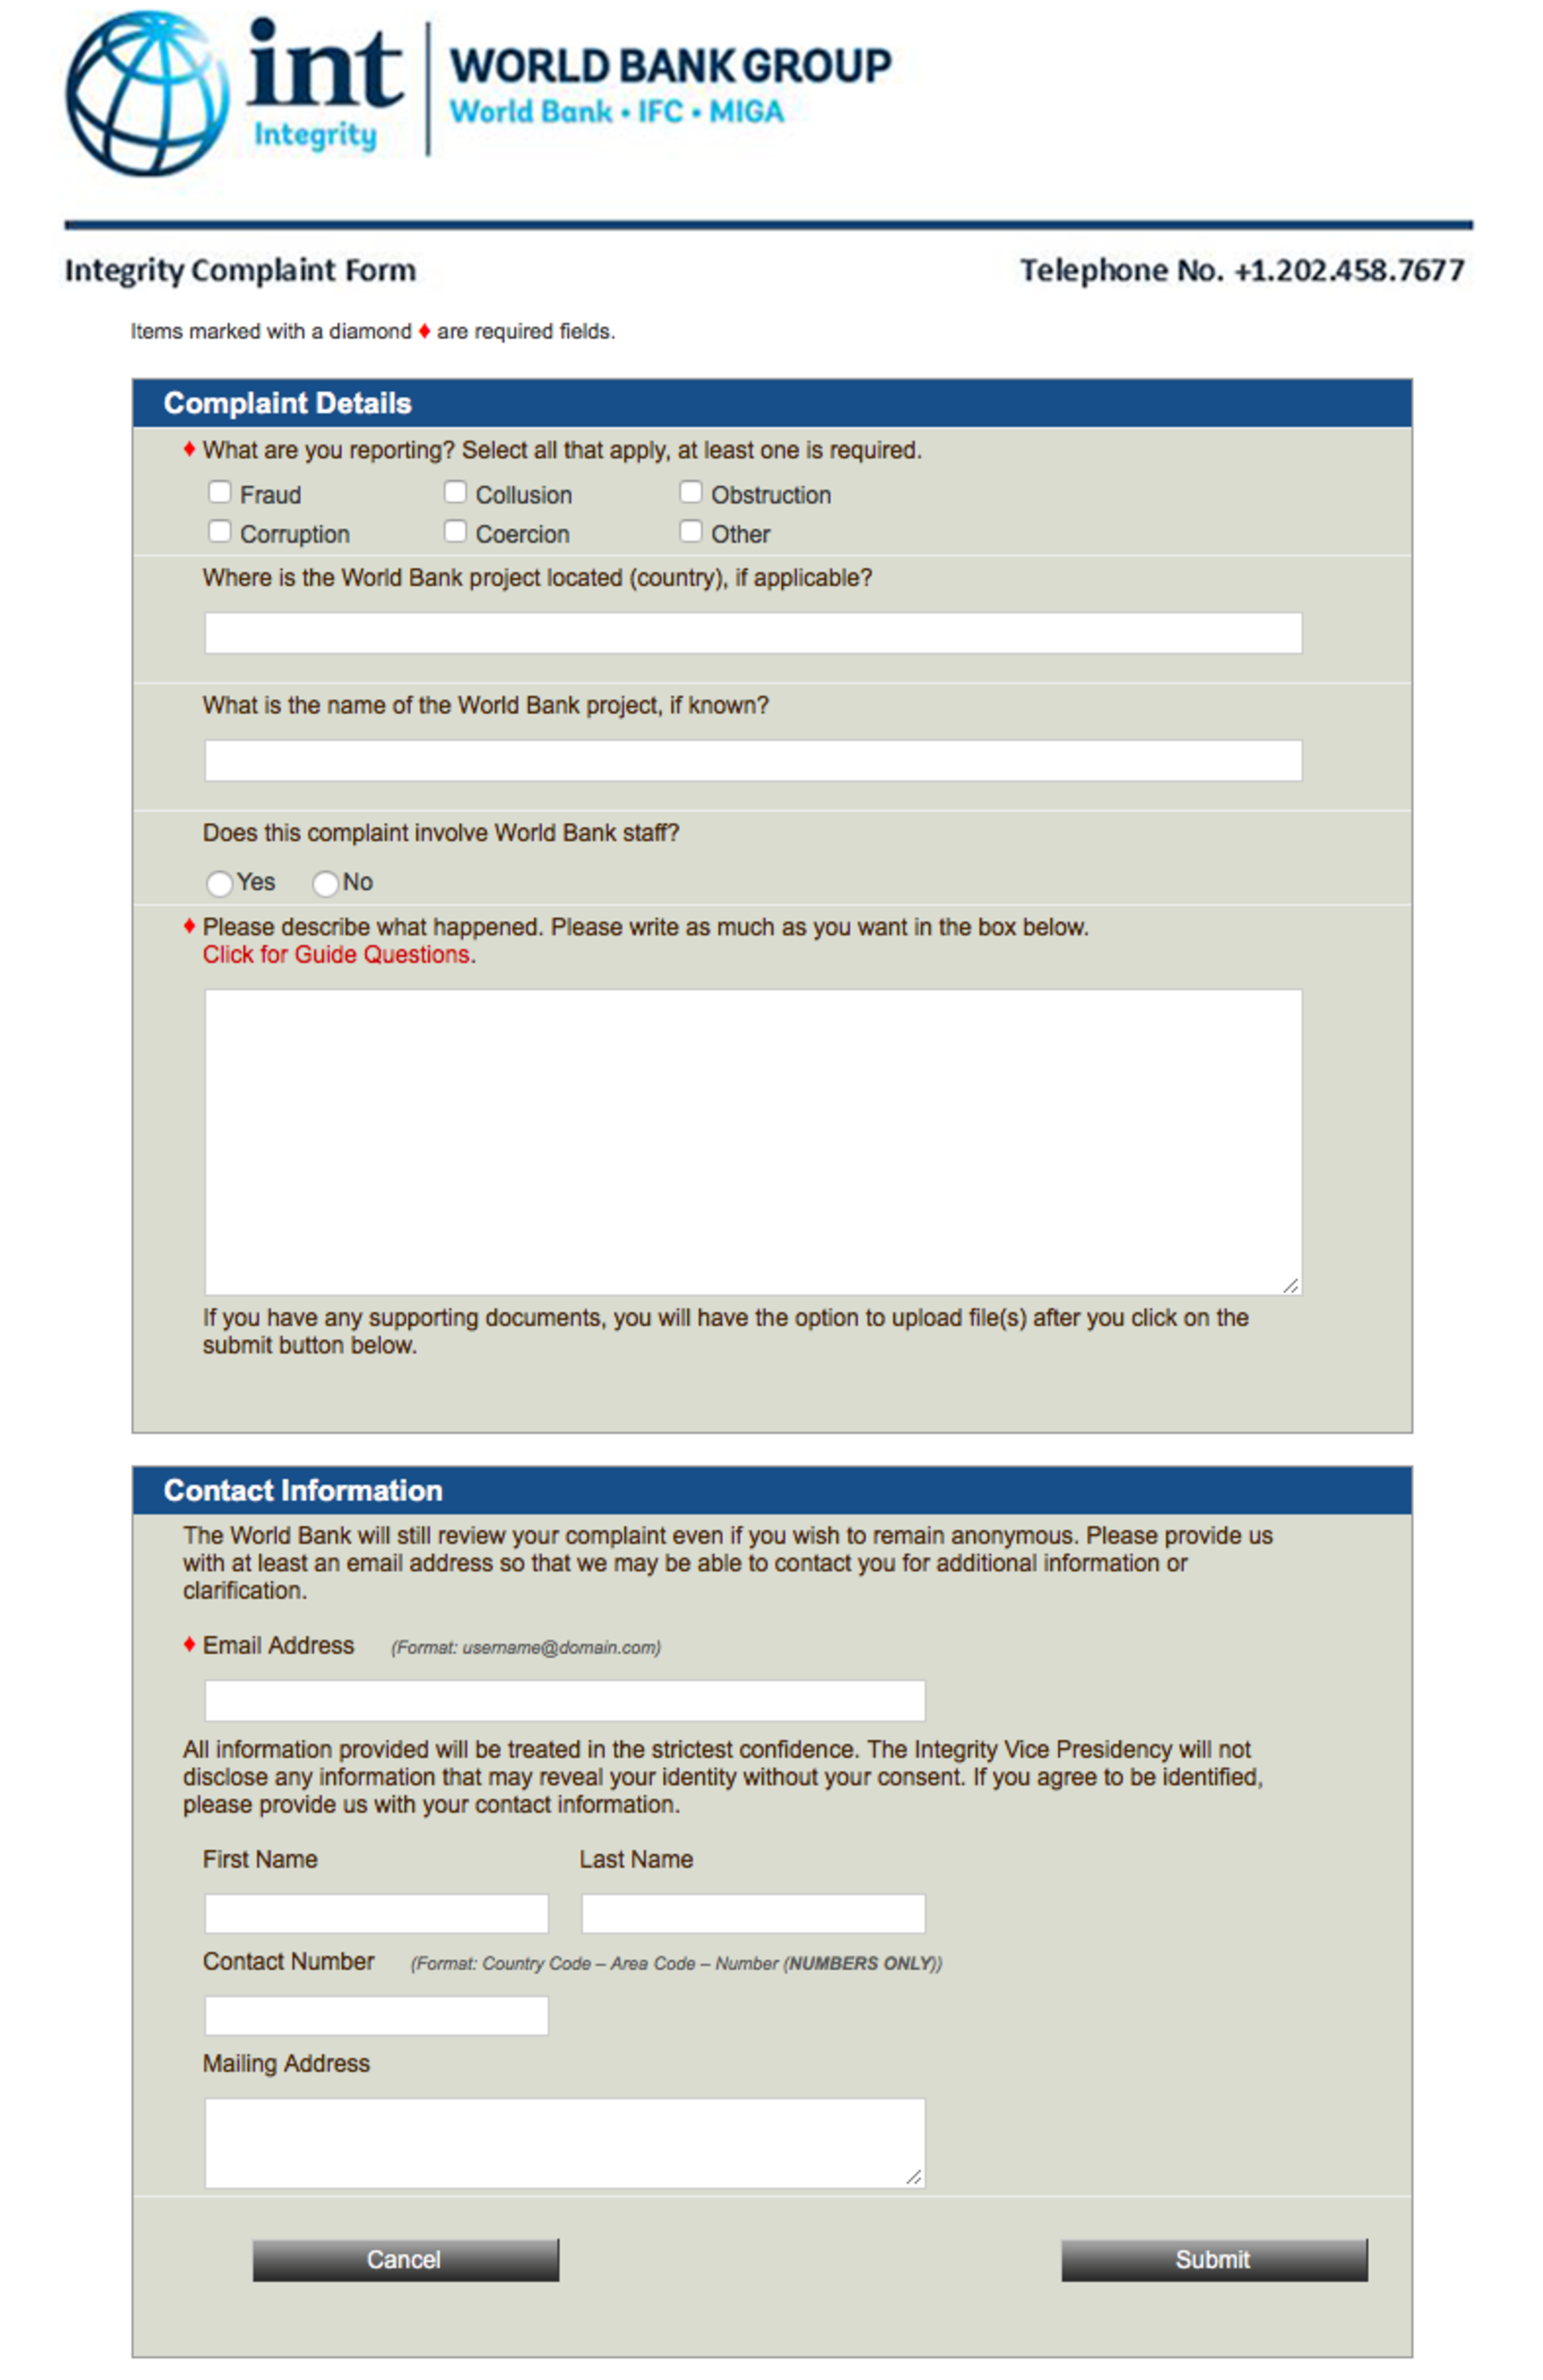
\includegraphics[max width=.75\textwidth]{../img/wb_report_complaint.pdf}
\end{center}
\noindent \footnotesize{\textbf{Source:} \cite{wb_complaint}}
\end{figure}


\section{Searching for \textit{red-flags}}

The real issue for the World Bank becomes that, in order for them to conduct a Complaint Intake, an Investigation Case, or even an Investigation Report, they rely on third parties. As seen in the online form that the World Bank provides, figure  \ref{fig_complaint} and on the mobile application, they are making a significant effort to supply third parties with the best tools to report any cases of corruption, fraud, collusion, coercion and  obstruction so that reporting do not becomes the obstacle. Having said that, the real problem for The World Bank becomes that their efforts to conduct investigations is limited to the information they receive from third parties. This is an important matter when their objective is to reduce the world's poverty by awarding procurements, loans and credit to developing countries and at the same time they are facing corruption, fraud and collusion problems by which only few sectors are being benefited.

Investigators at the World Bank's Integrity Vice Presidency (INT) are responsible for investigating collusion, as well as the other sanctionable offenses of coercion, fraud and corruption in World Bank-financed projects. The challenge with a global portfolio is how to detect collusion or corruption, particularly if no one reports the incident.

For this reason, The World Banks has made an effort in order to conduct a new type of investigations that do not depend on third parties but depends on data. The problem now becomes: how to identify corruption, collusion, fraud, coercion and obstruction by looking on data? The World Bank has some initial thoughts and has been trying to search for new and innovative ways to tackle this problem. For example, on June 2014 they organized a DataSprint event that helped them to dive into data to address these type problems. The objective was to analyze, visualize, and mash-up the the data. We went to Washington, D.C. for several days of meetings and collaboration with the project partners at INT and the World Bank's Office of the Controller. The trip was an opportunity to learn what corruption, fraud, and collusion looks like in the data.

INT investigators have identified several patterns in bidding behavior that could point to collusion or other forms of corruption. Regular, periodic rotation of contract awards among a small group of contractors, for example, might indicate that bidders are working together to set prices or distribute contracts. Contractors may split large projects into multiple small ones, keeping individual contract values below a threshold that triggers additional review or competitive bidding. The total number of bidders shrinking over time might indicate that potential contractors are being pushed out of the market through some form of illegal coercion. While none of these findings represent clear-cut evidence of collusion, they are detectable clues that can help direct investigative efforts and ensure that the integrity of development is not compromised \parencite{dssg_proc}.

The INT developed a visualization, shown on figure \ref{fig_what_corr}, that shows cases that suggests malicious practices. To start with, sub-figure \ref{fig_cum_value} shows data that corresponds to a case in which  six suppliers that are supposed to be competitive and all the cumulative value on non-competitive contracts are being assigned to suppler number one. On sub-figure \ref{fig_value} it is shown that contracts, that correspond to Company A, numbers one and two overcome the threshold for a common competitive biding. This might be suggesting collusion. Sub-figure \ref{fig_winning} shows a case where suppliers four to eight always bid a little less that the winning bid suggesting another type of collusion. Now, on sub-figure \ref{fig_month} there is a suggestion of favoritism that suggest corruption or even coercion in which the value of a non-competitive contract goes high exactly in the times of a governmental election. Sub-figure \ref{fig_links} suggests that companies that have contracts or directors in common with other companies that have been previously debarred are suspicious of malicious activities. As it can be seen from sub-figures 
\ref{fig_bid1} and \ref{fig_bid2} there tend to be bidding patterns in which take turns by bidding differently in each round such that they take turns to get the contracts. This affects directly the process making them non competitive when they should be competitive. Lastly, it can be seen on figure \ref{fig_proposals} that as time pass, only two suppliers are the ones participating on proposals among a vast pool. This  fact is suggesting that those two suppliers might have done something  to coerce the others not to participate on proposals after time four.

\begin{figure}[H]
\begin{center}
\caption{What does corruption look like?}
\includegraphics[max width=0.6\textwidth]{../img/poster_what.pdf}
\label{fig_what_corr}
\end{center}


\begin{subfigure}[t]{0.5\textwidth}
\caption{Cumulative value of non-competitive contracts}
\label{fig_cum_value}
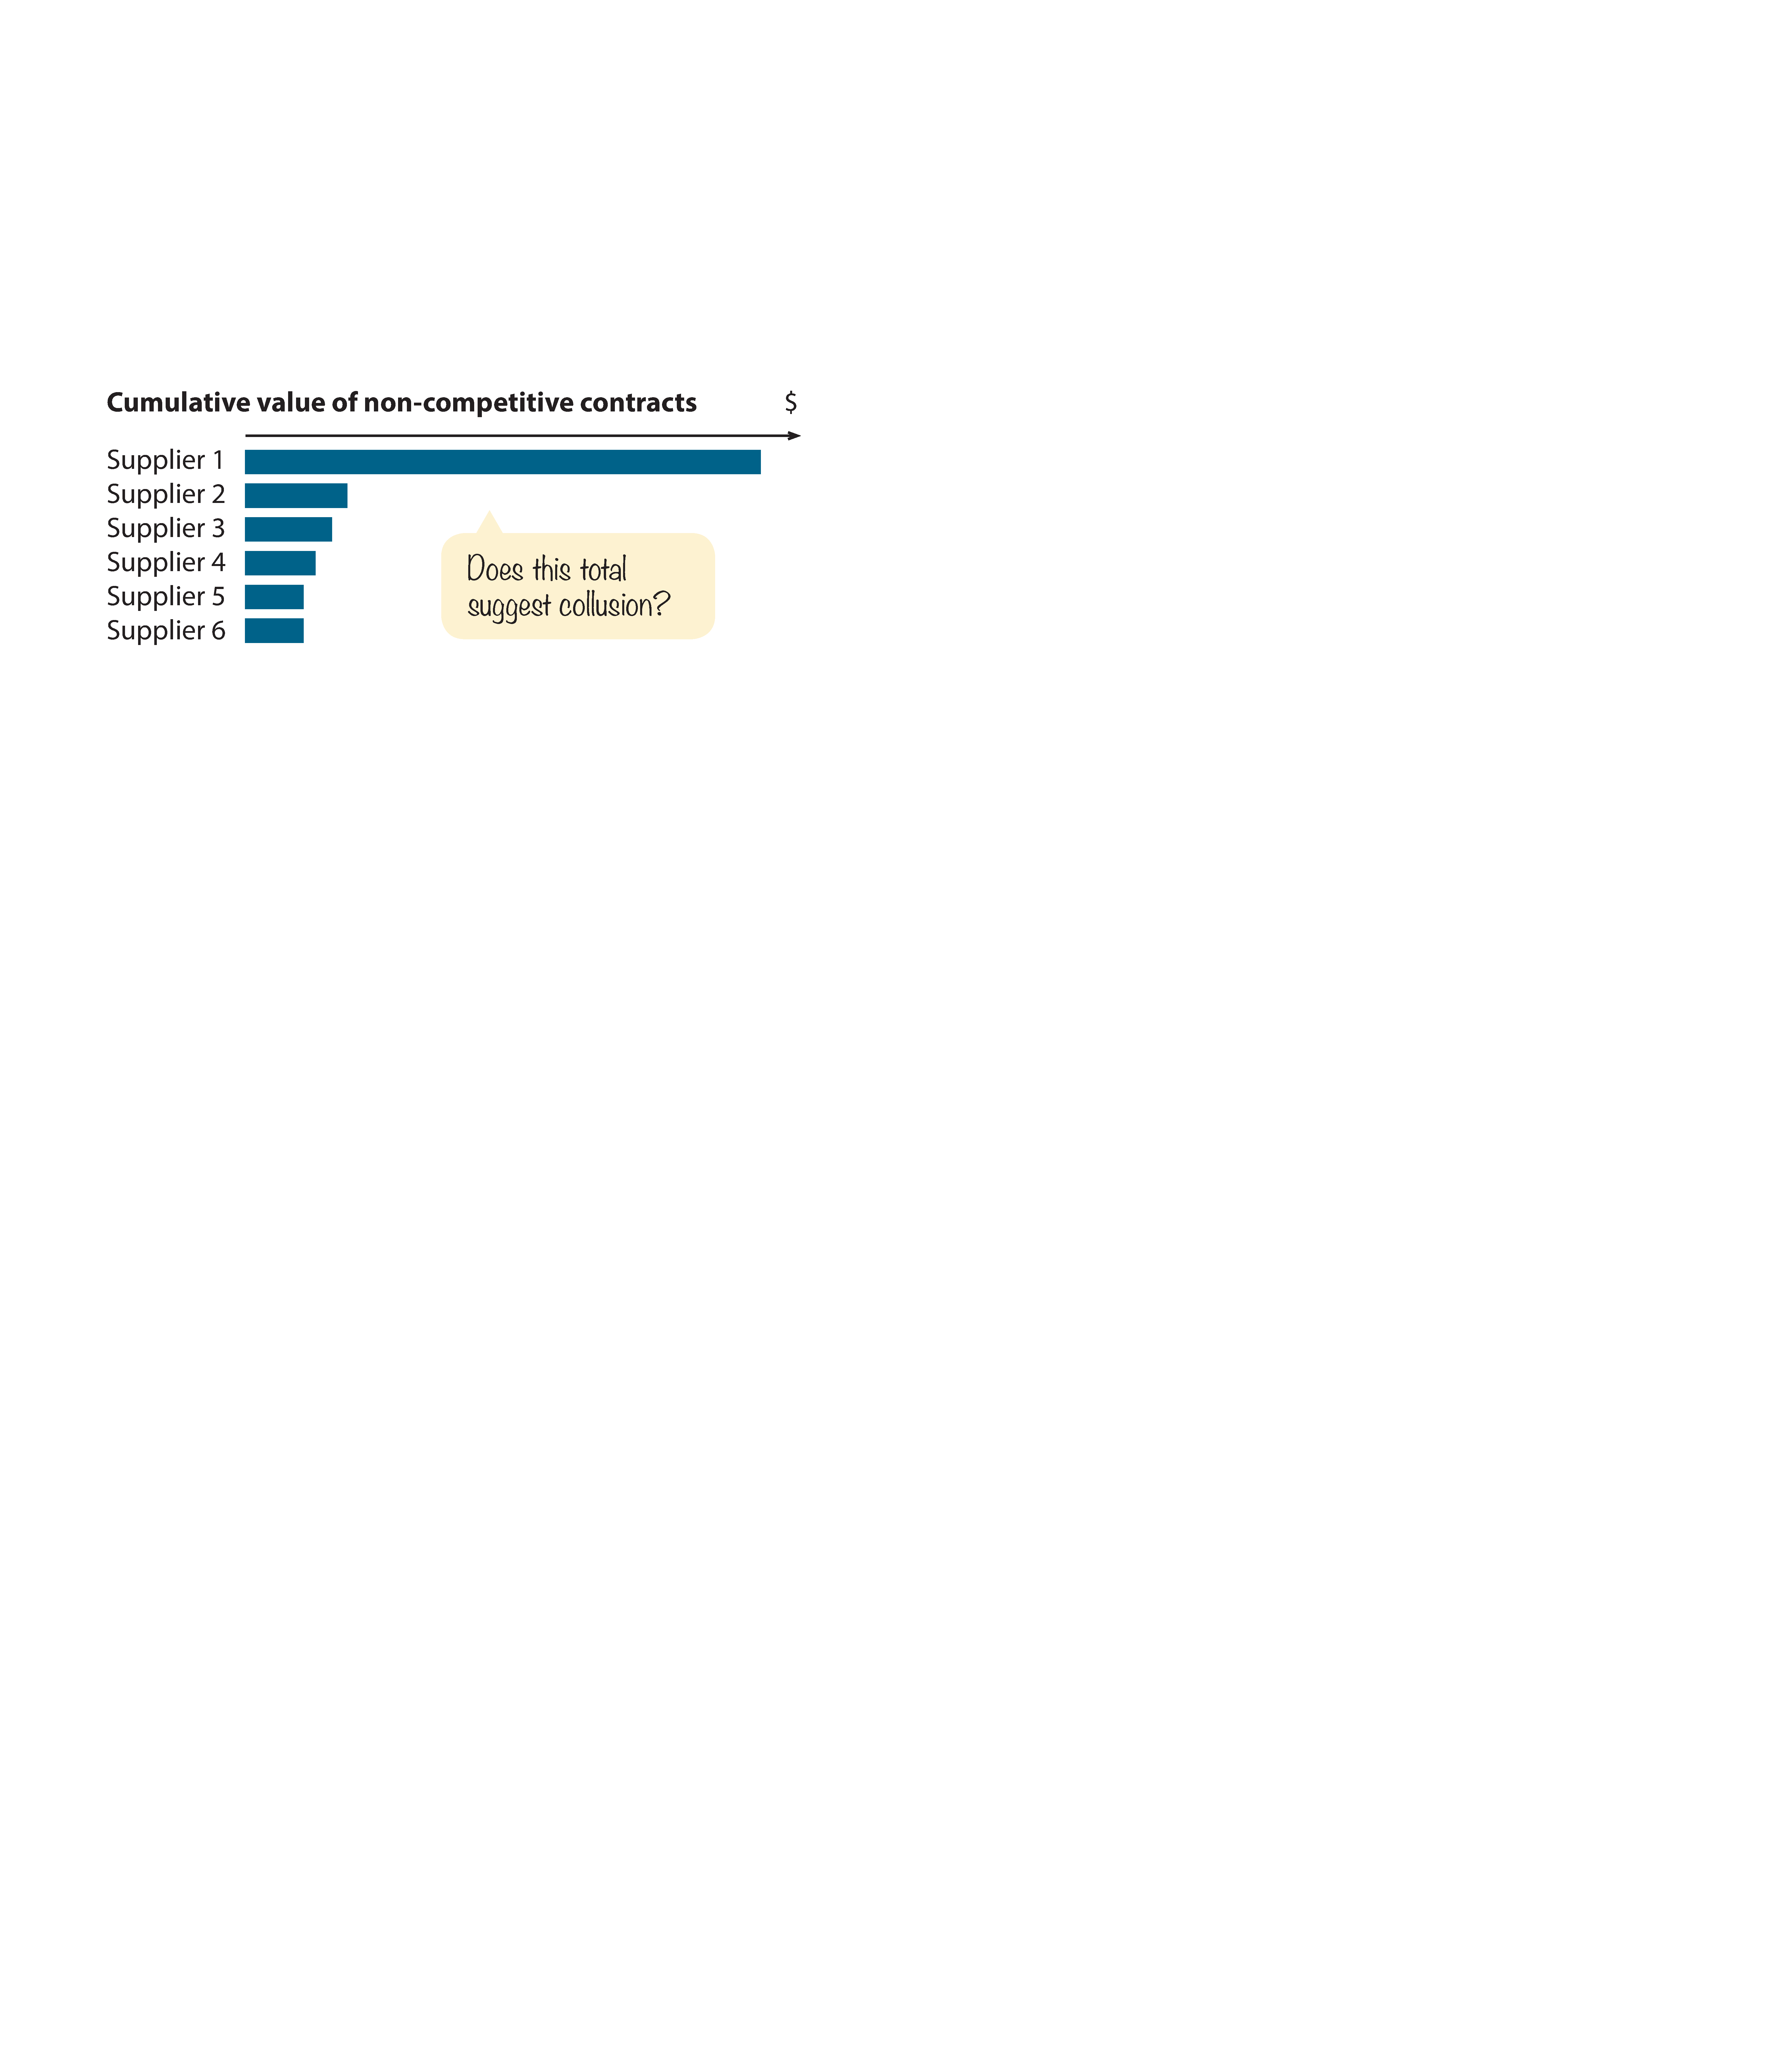
\includegraphics[max width=1\textwidth]{../img/poster_cumulative_value.pdf}
\end{subfigure}
~
\begin{subfigure}[t]{0.5\textwidth}
\caption{Value of Contracts}
\label{fig_value}
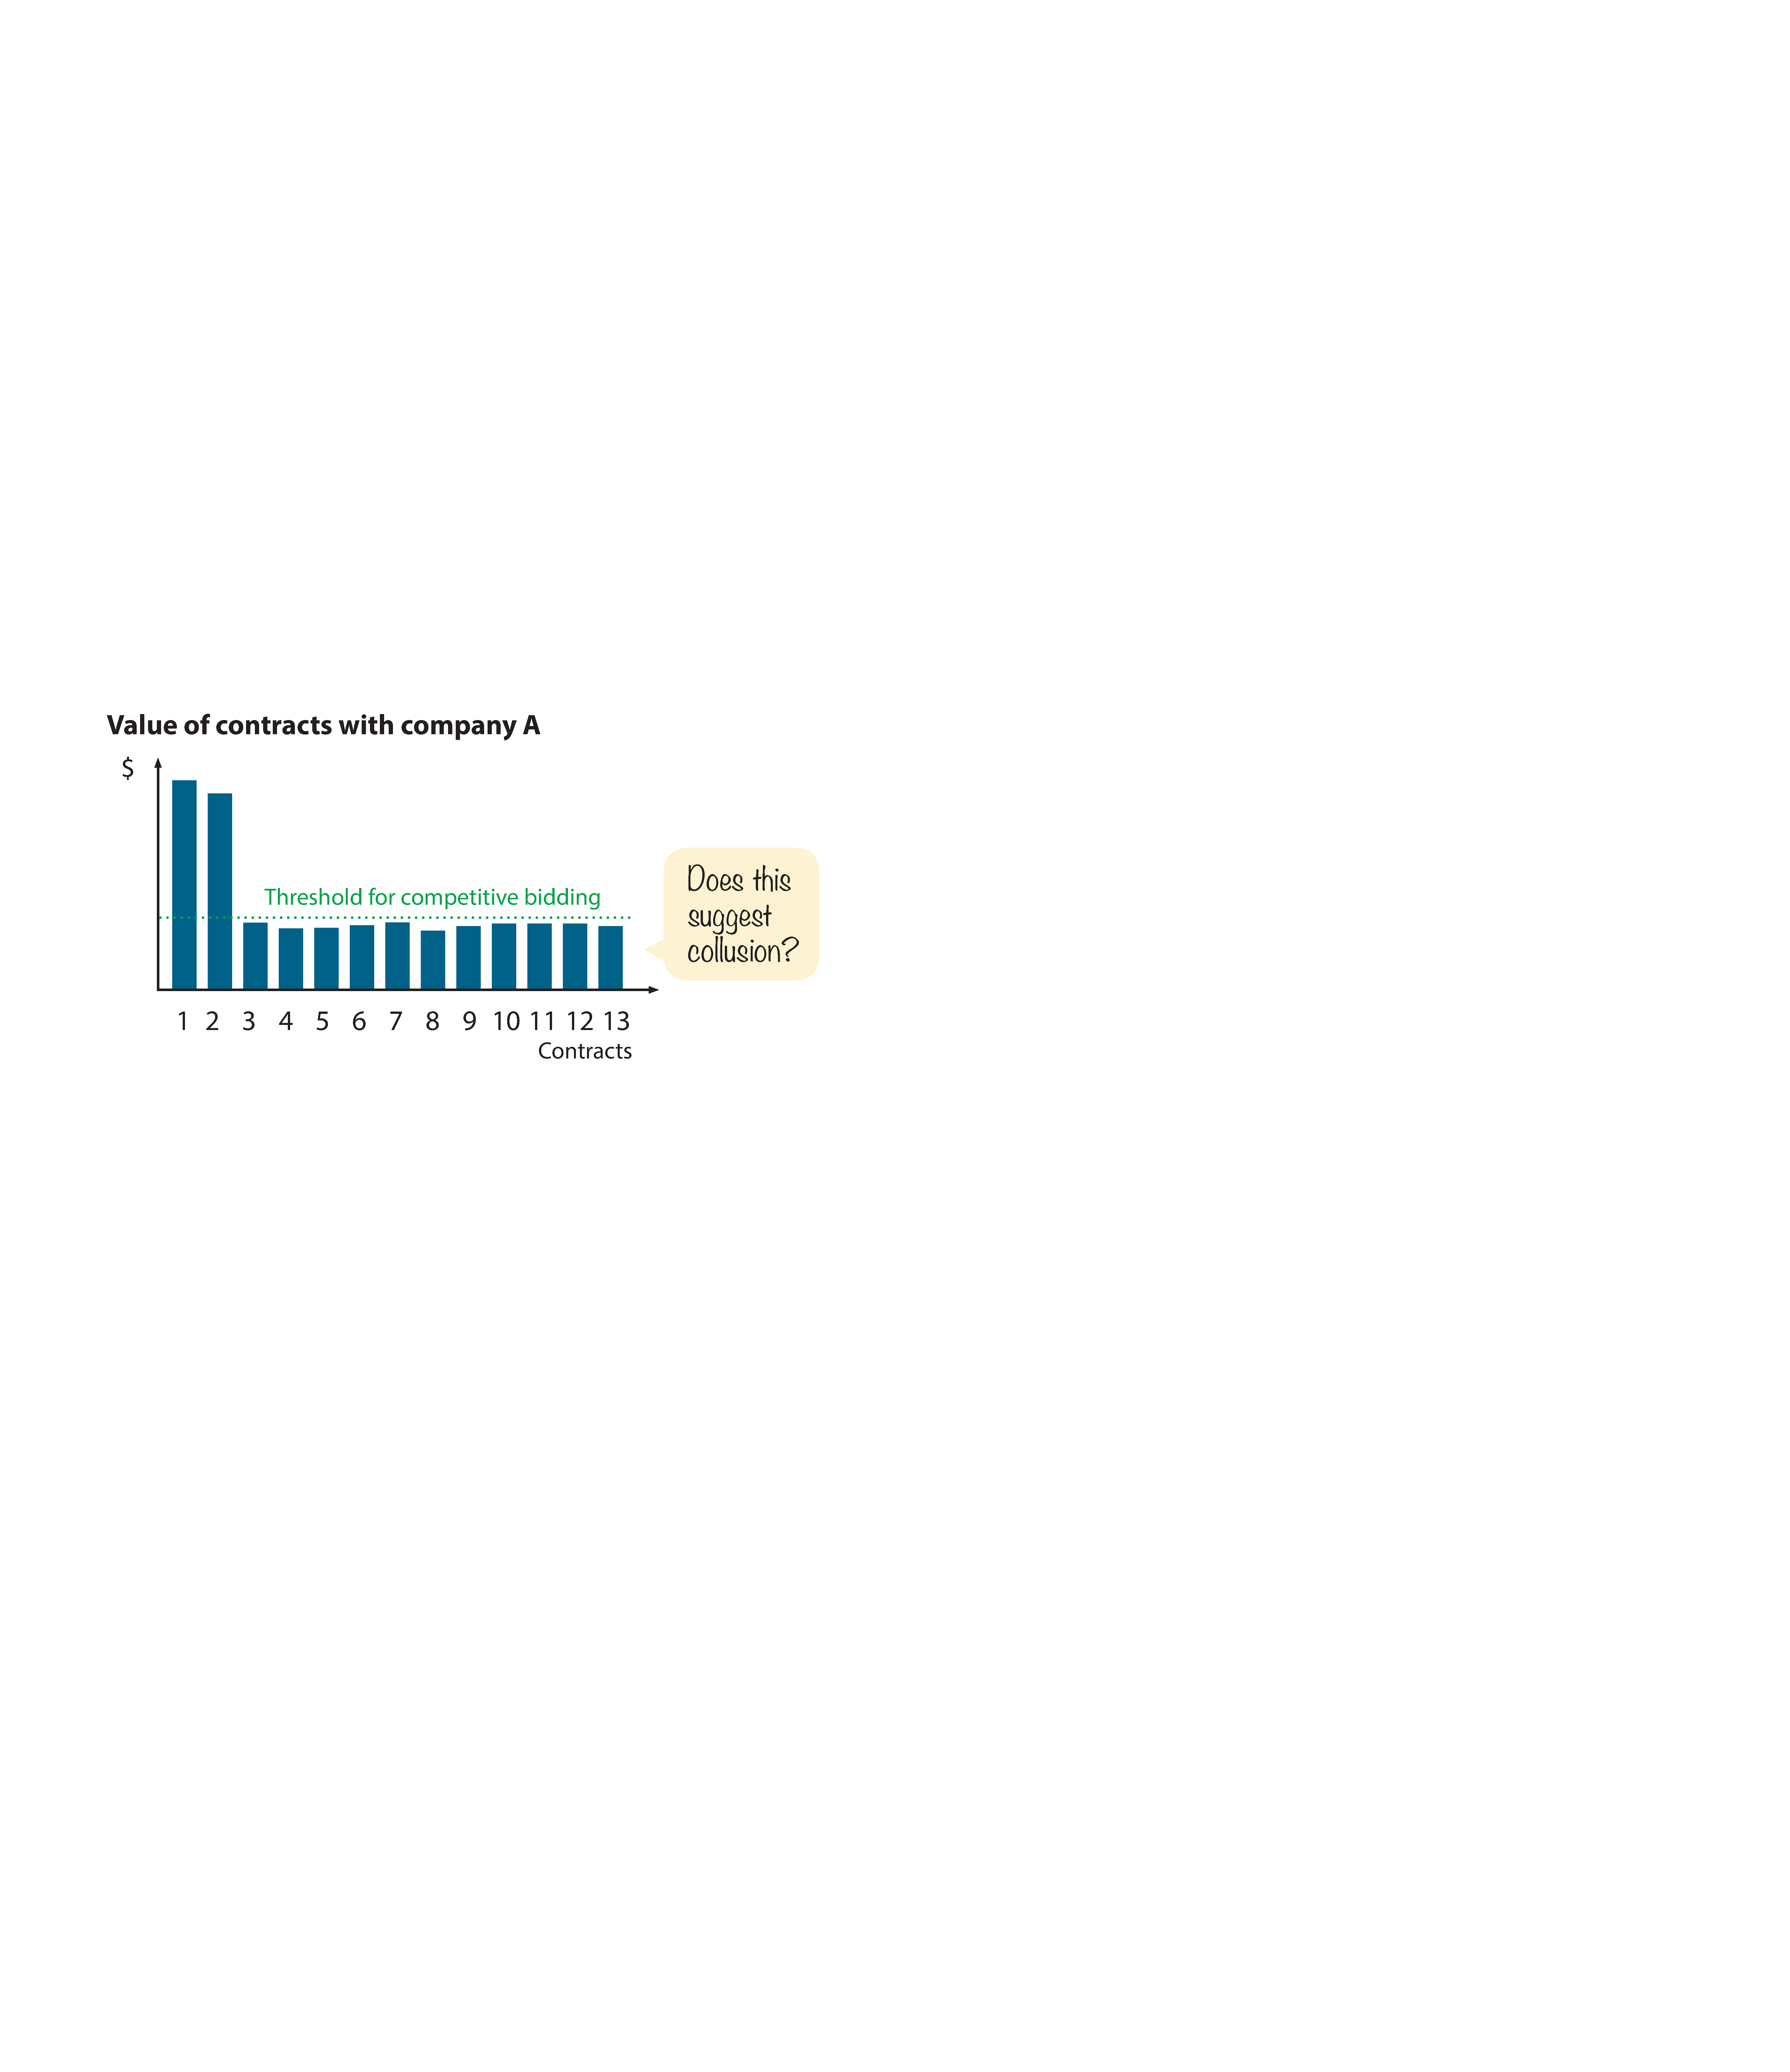
\includegraphics[max width=1\textwidth]{../img/poster_value.pdf}
\end{subfigure}
~
\begin{subfigure}[t]{0.5\textwidth}
\caption{Winning patterns}
\label{fig_winning}
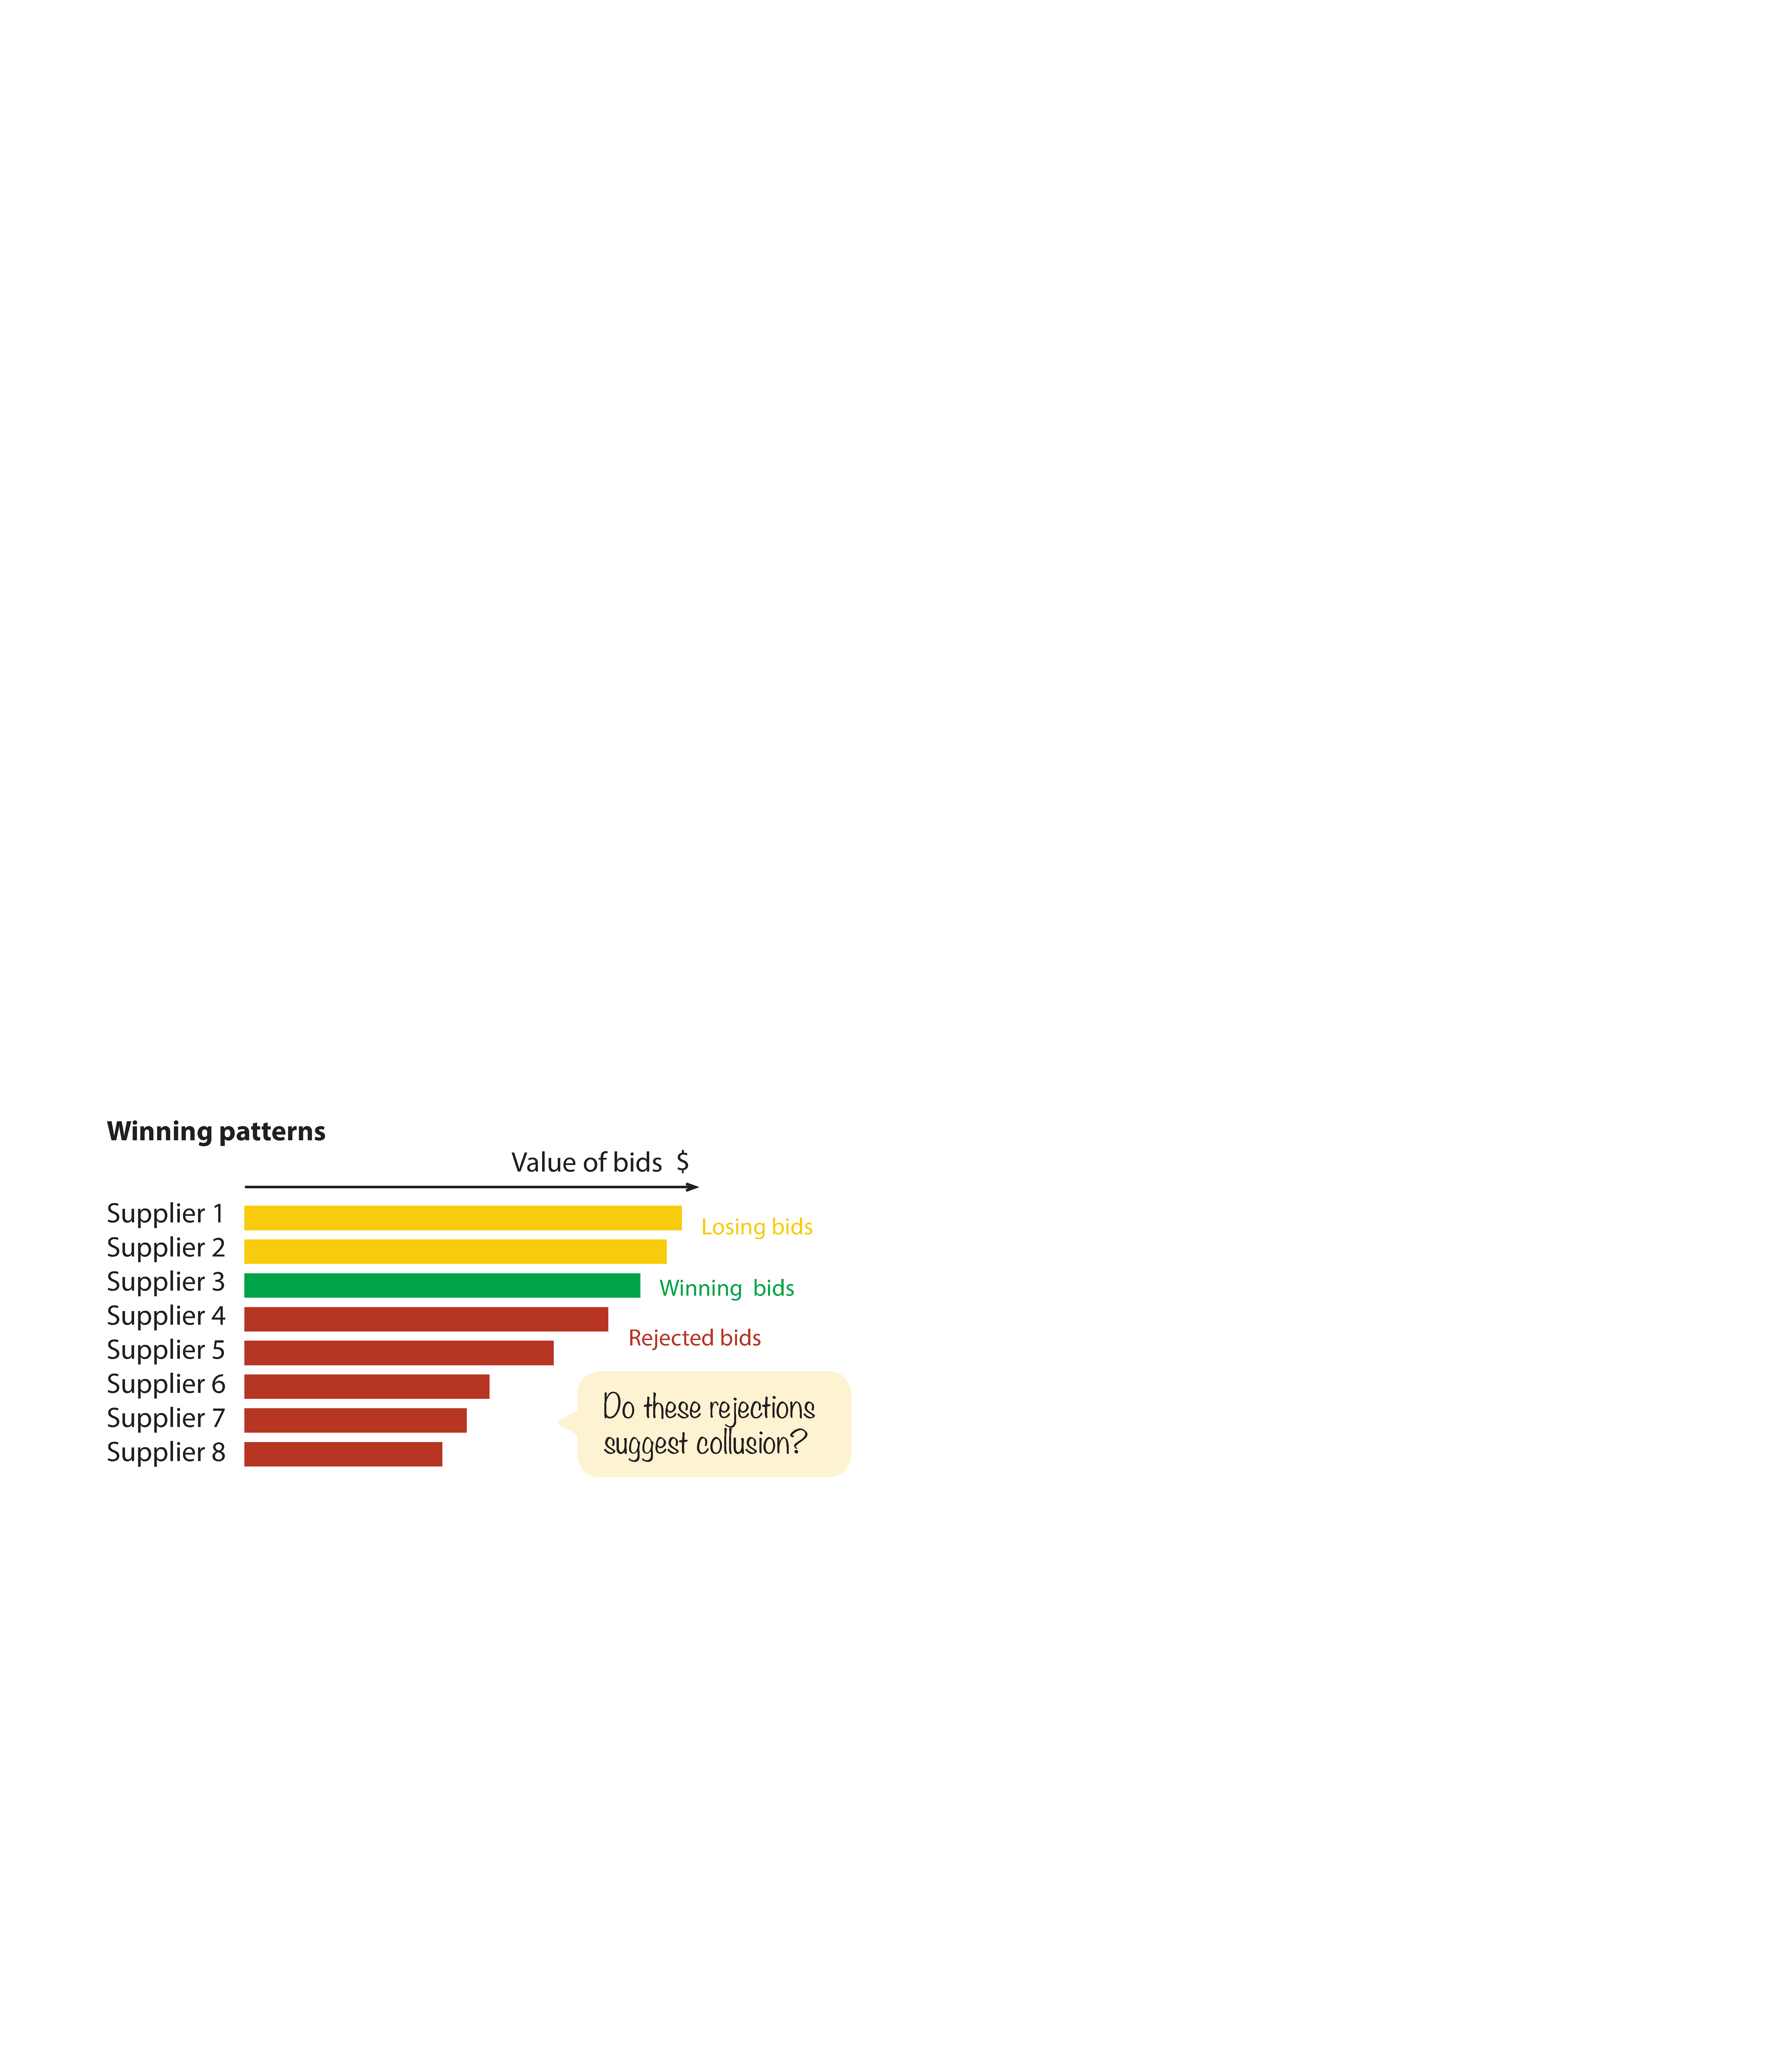
\includegraphics[max width=1\textwidth]{../img/poster_winning_patterns.pdf}
\end{subfigure}
~
\begin{subfigure}[t]{0.5\textwidth}
\caption{Monthly value of non-competitive contracts}
\label{fig_month}
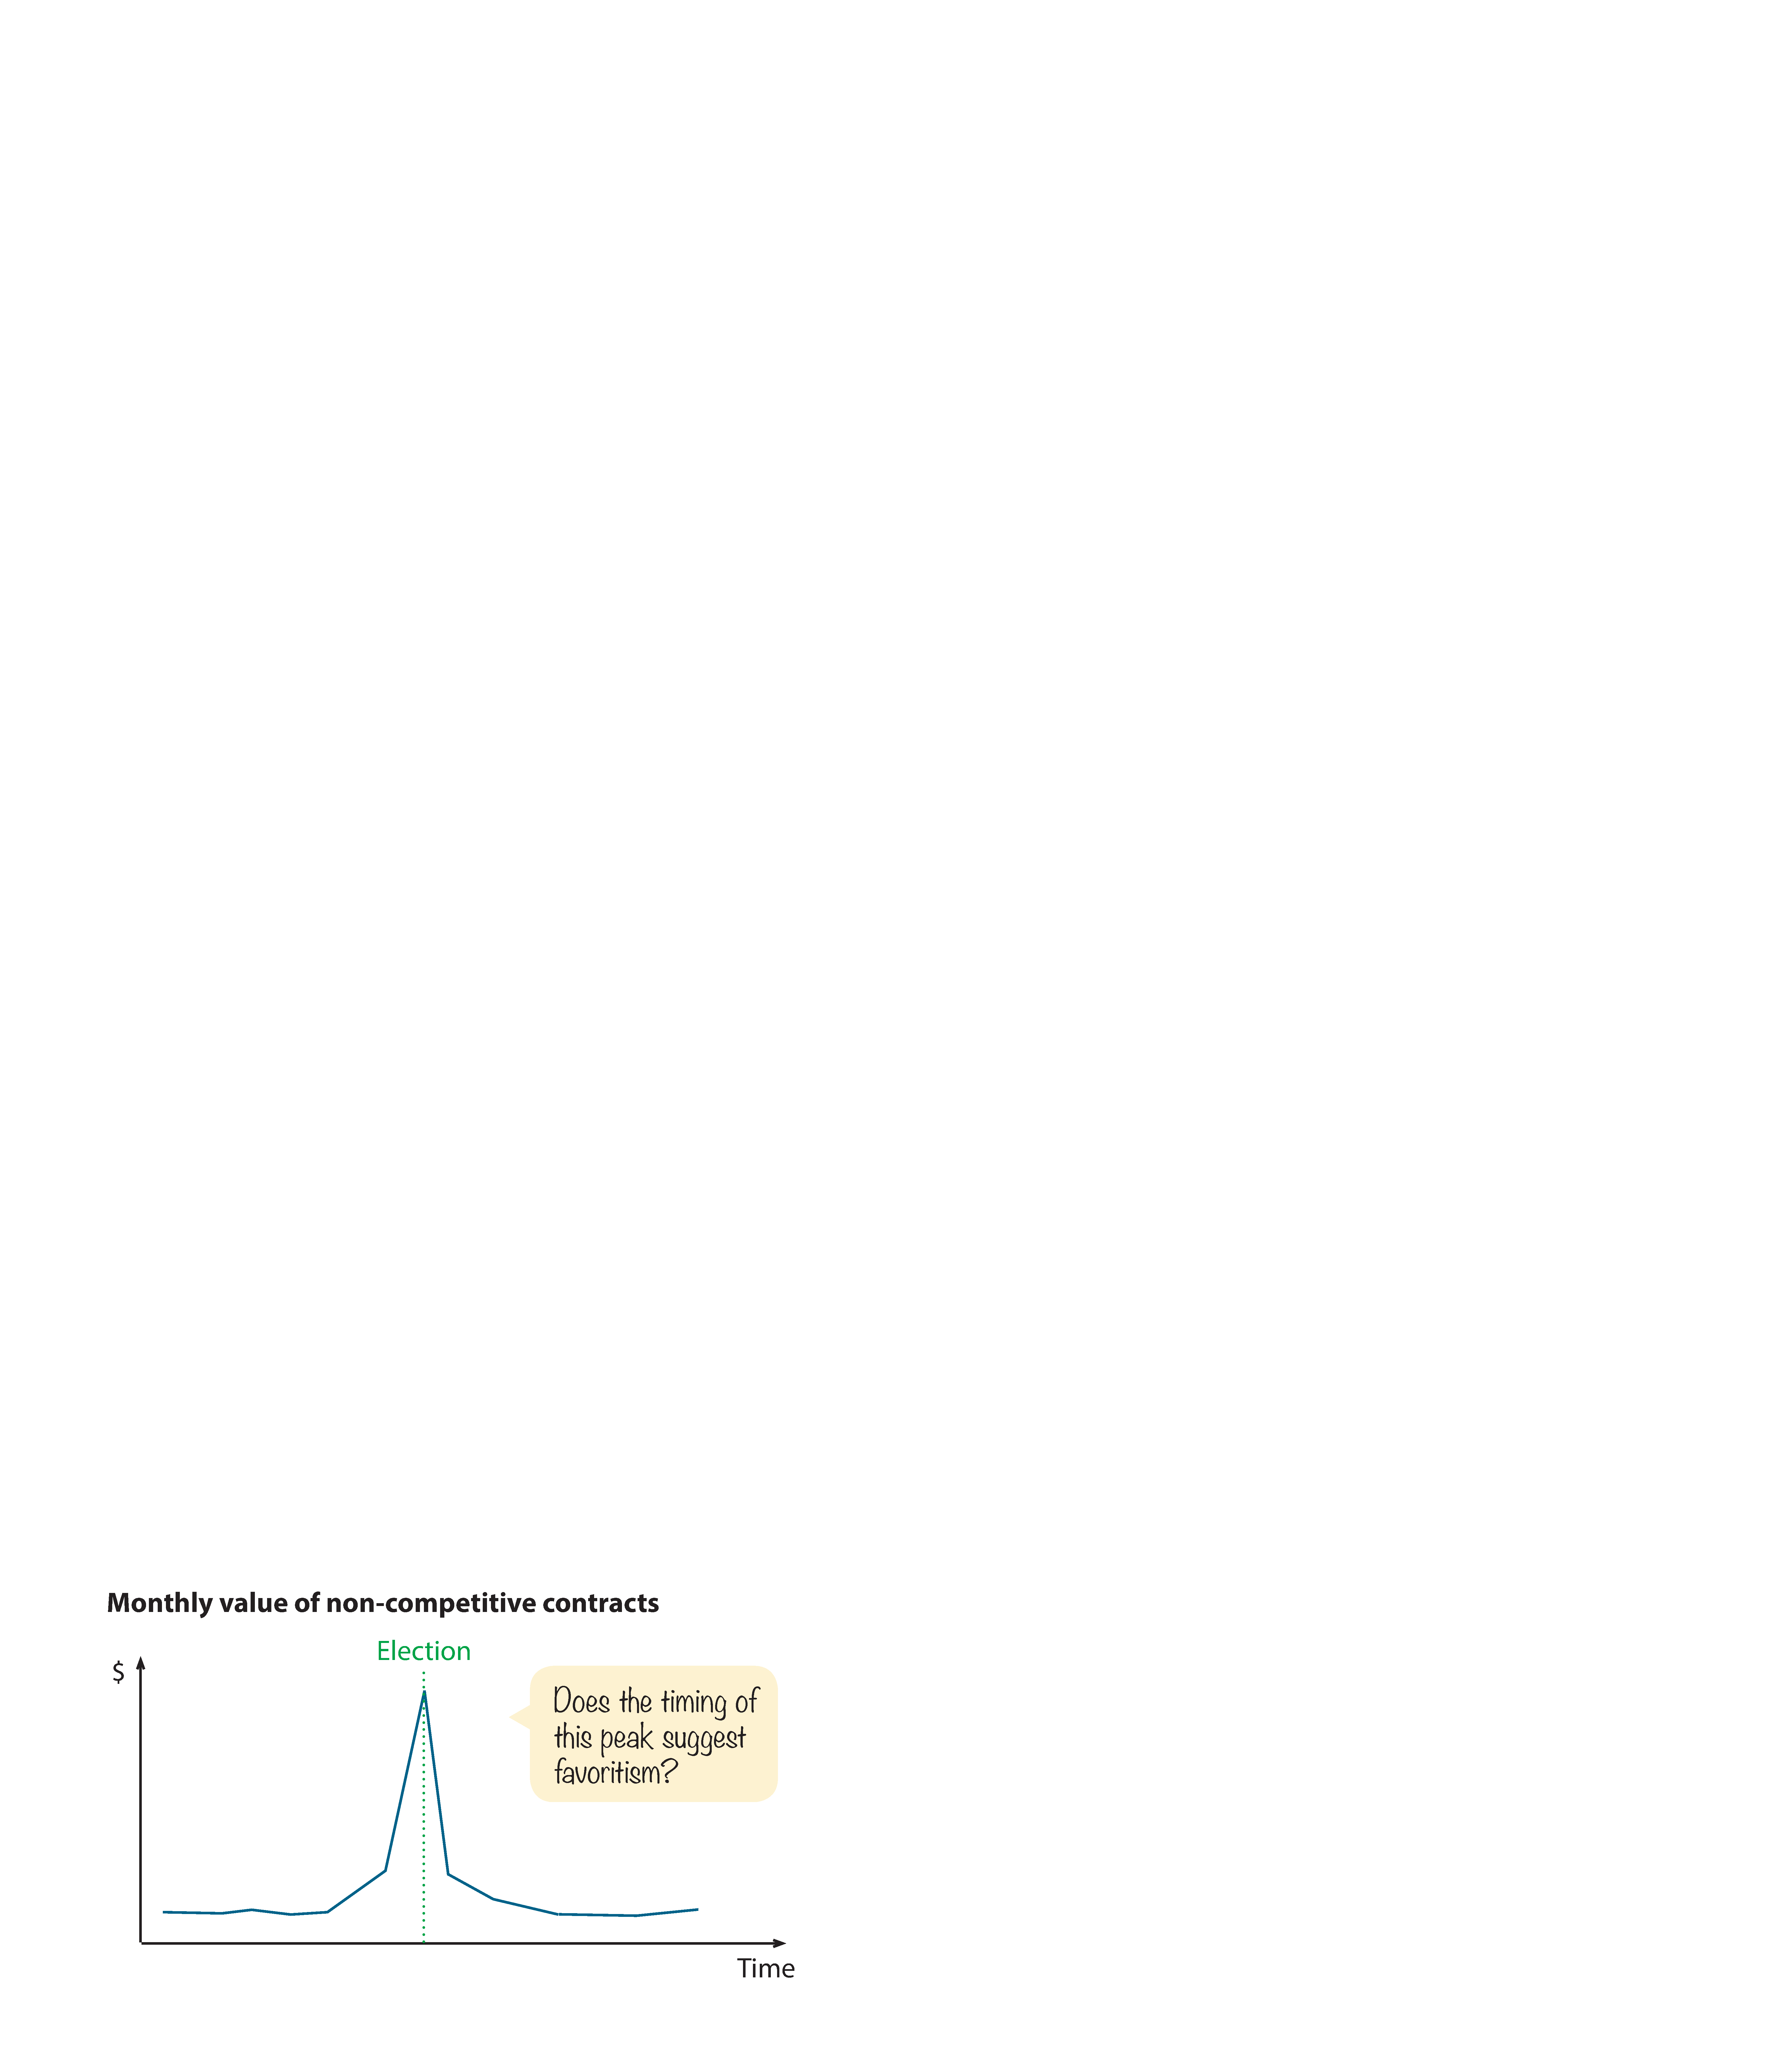
\includegraphics[max width=1\textwidth]{../img/poster_monthly.pdf}
\end{subfigure}
~
\begin{subfigure}[t]{0.5\textwidth}
\caption{Links between companies}
\label{fig_links}
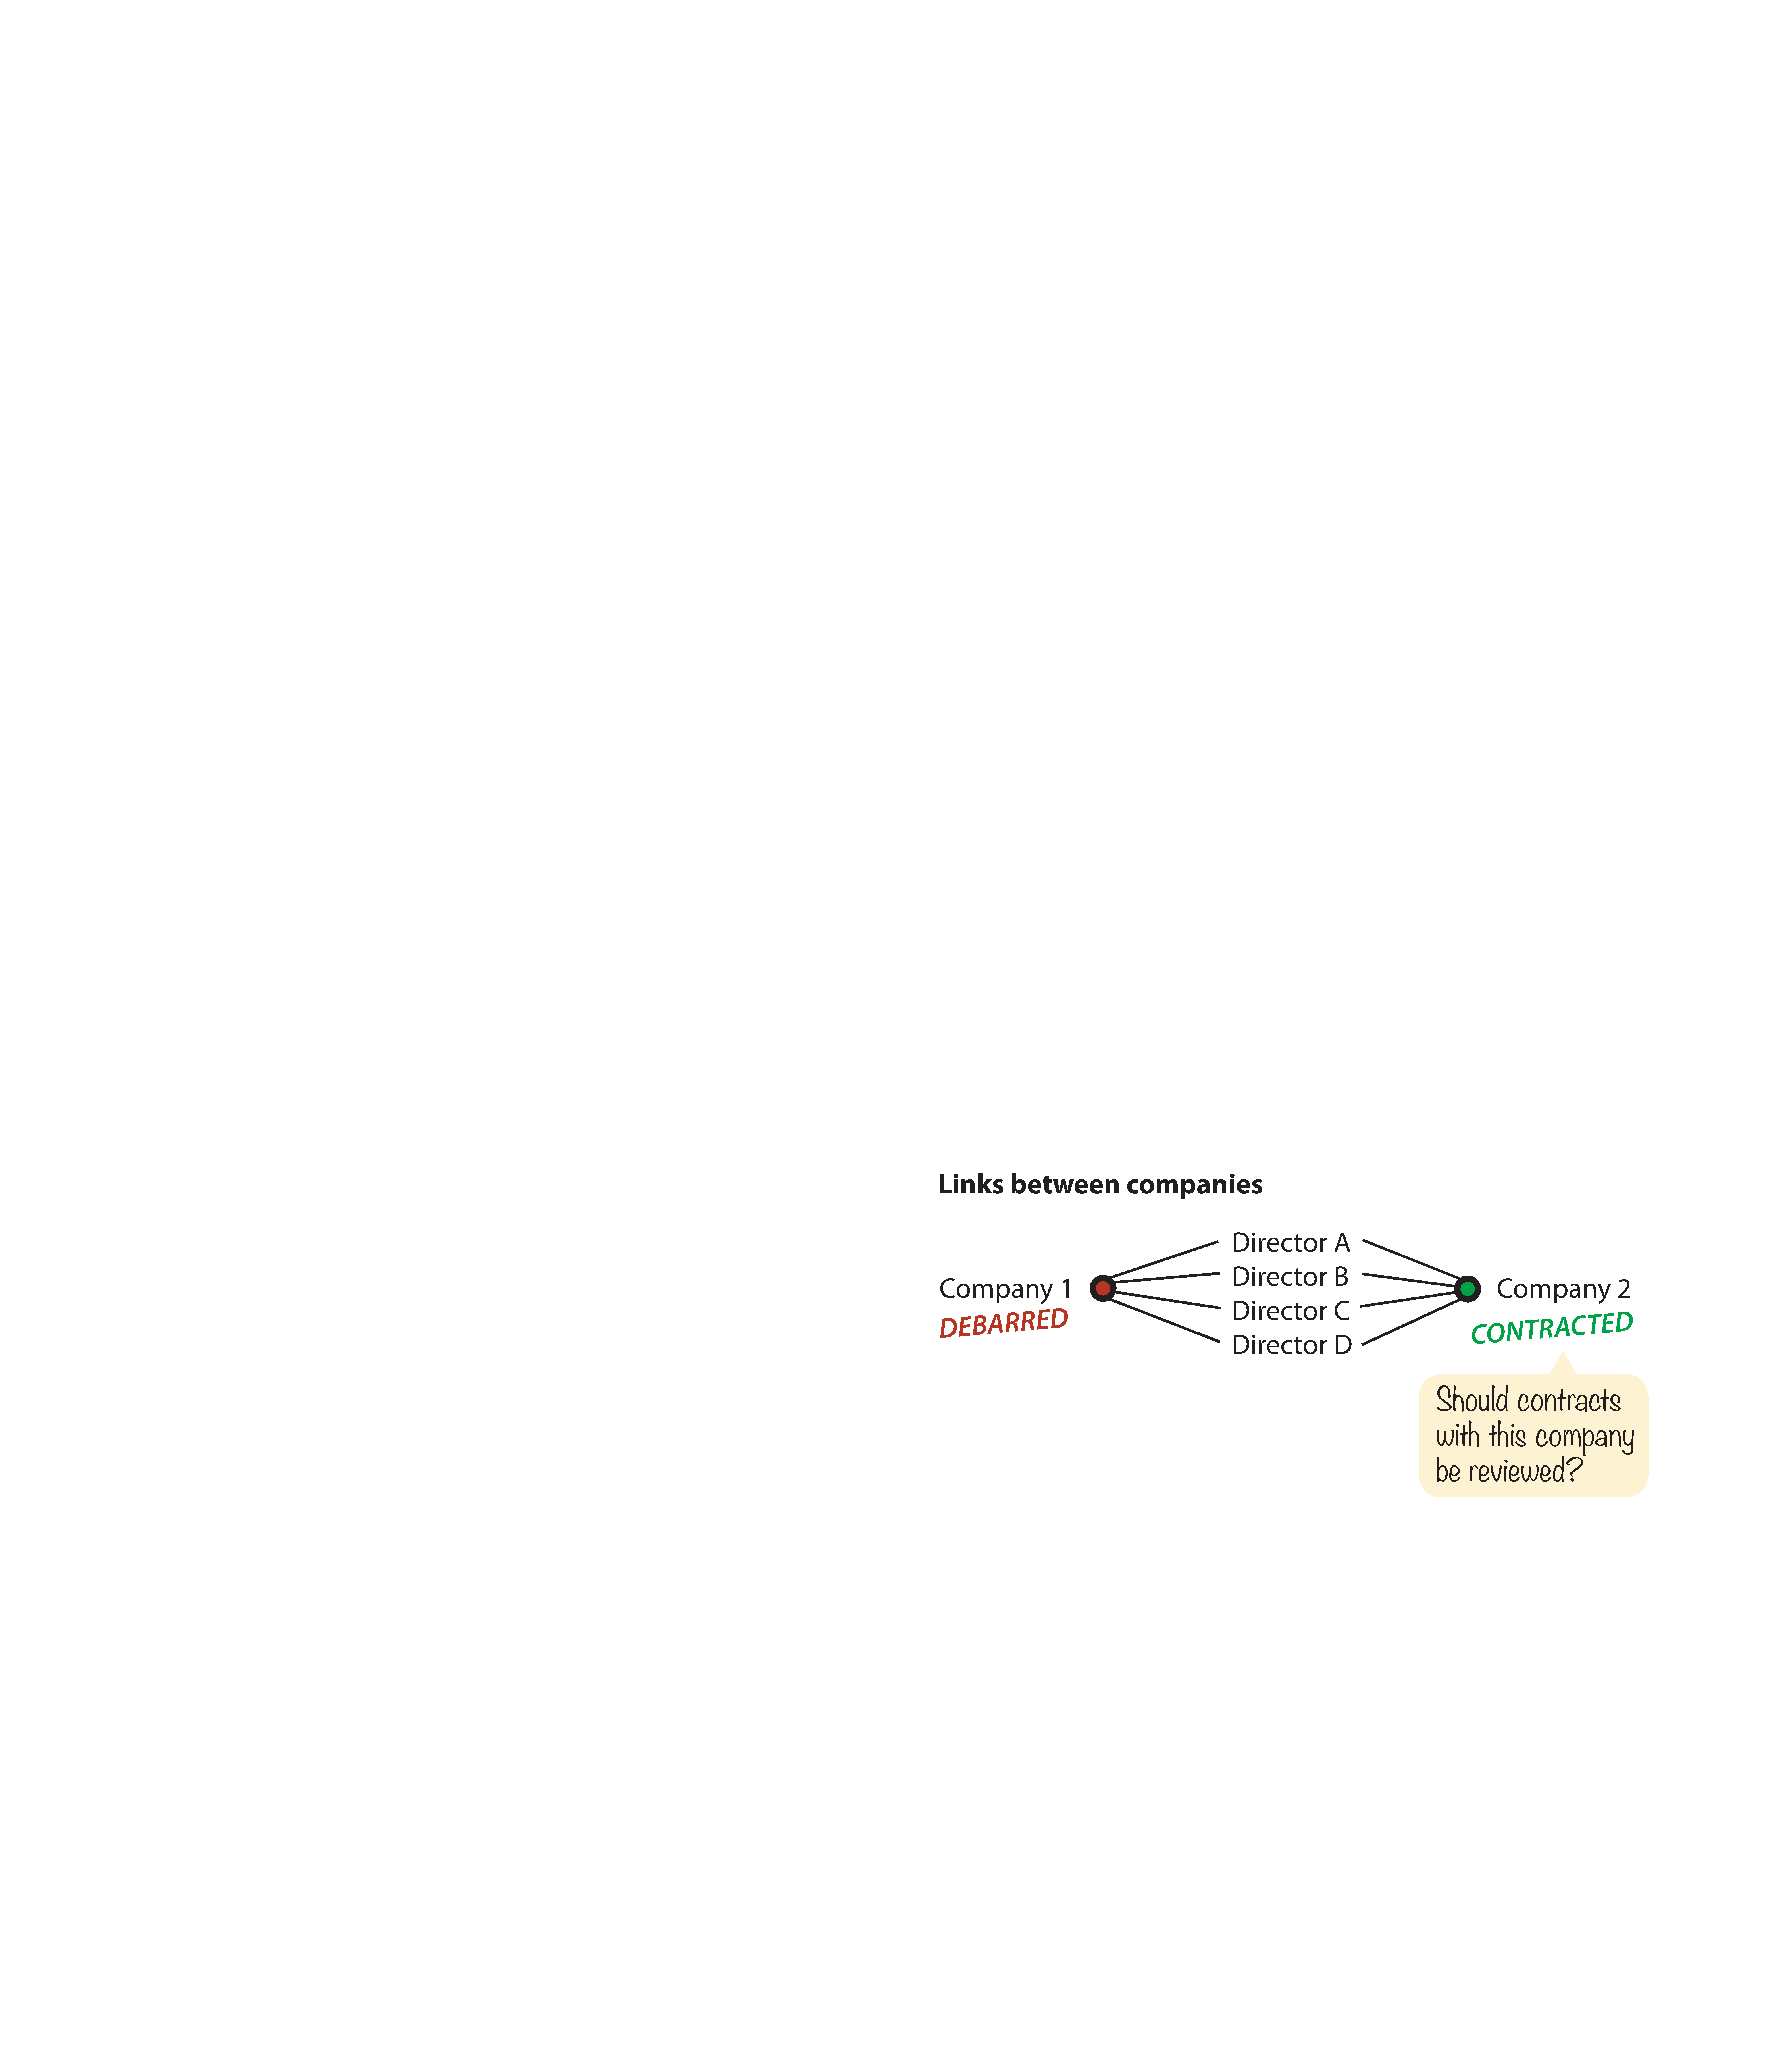
\includegraphics[max width=1\textwidth]{../img/poster_link.pdf}
\end{subfigure}
~
\begin{subfigure}[t]{0.5\textwidth}
\caption{Bidding patterns}
\label{fig_bid1}
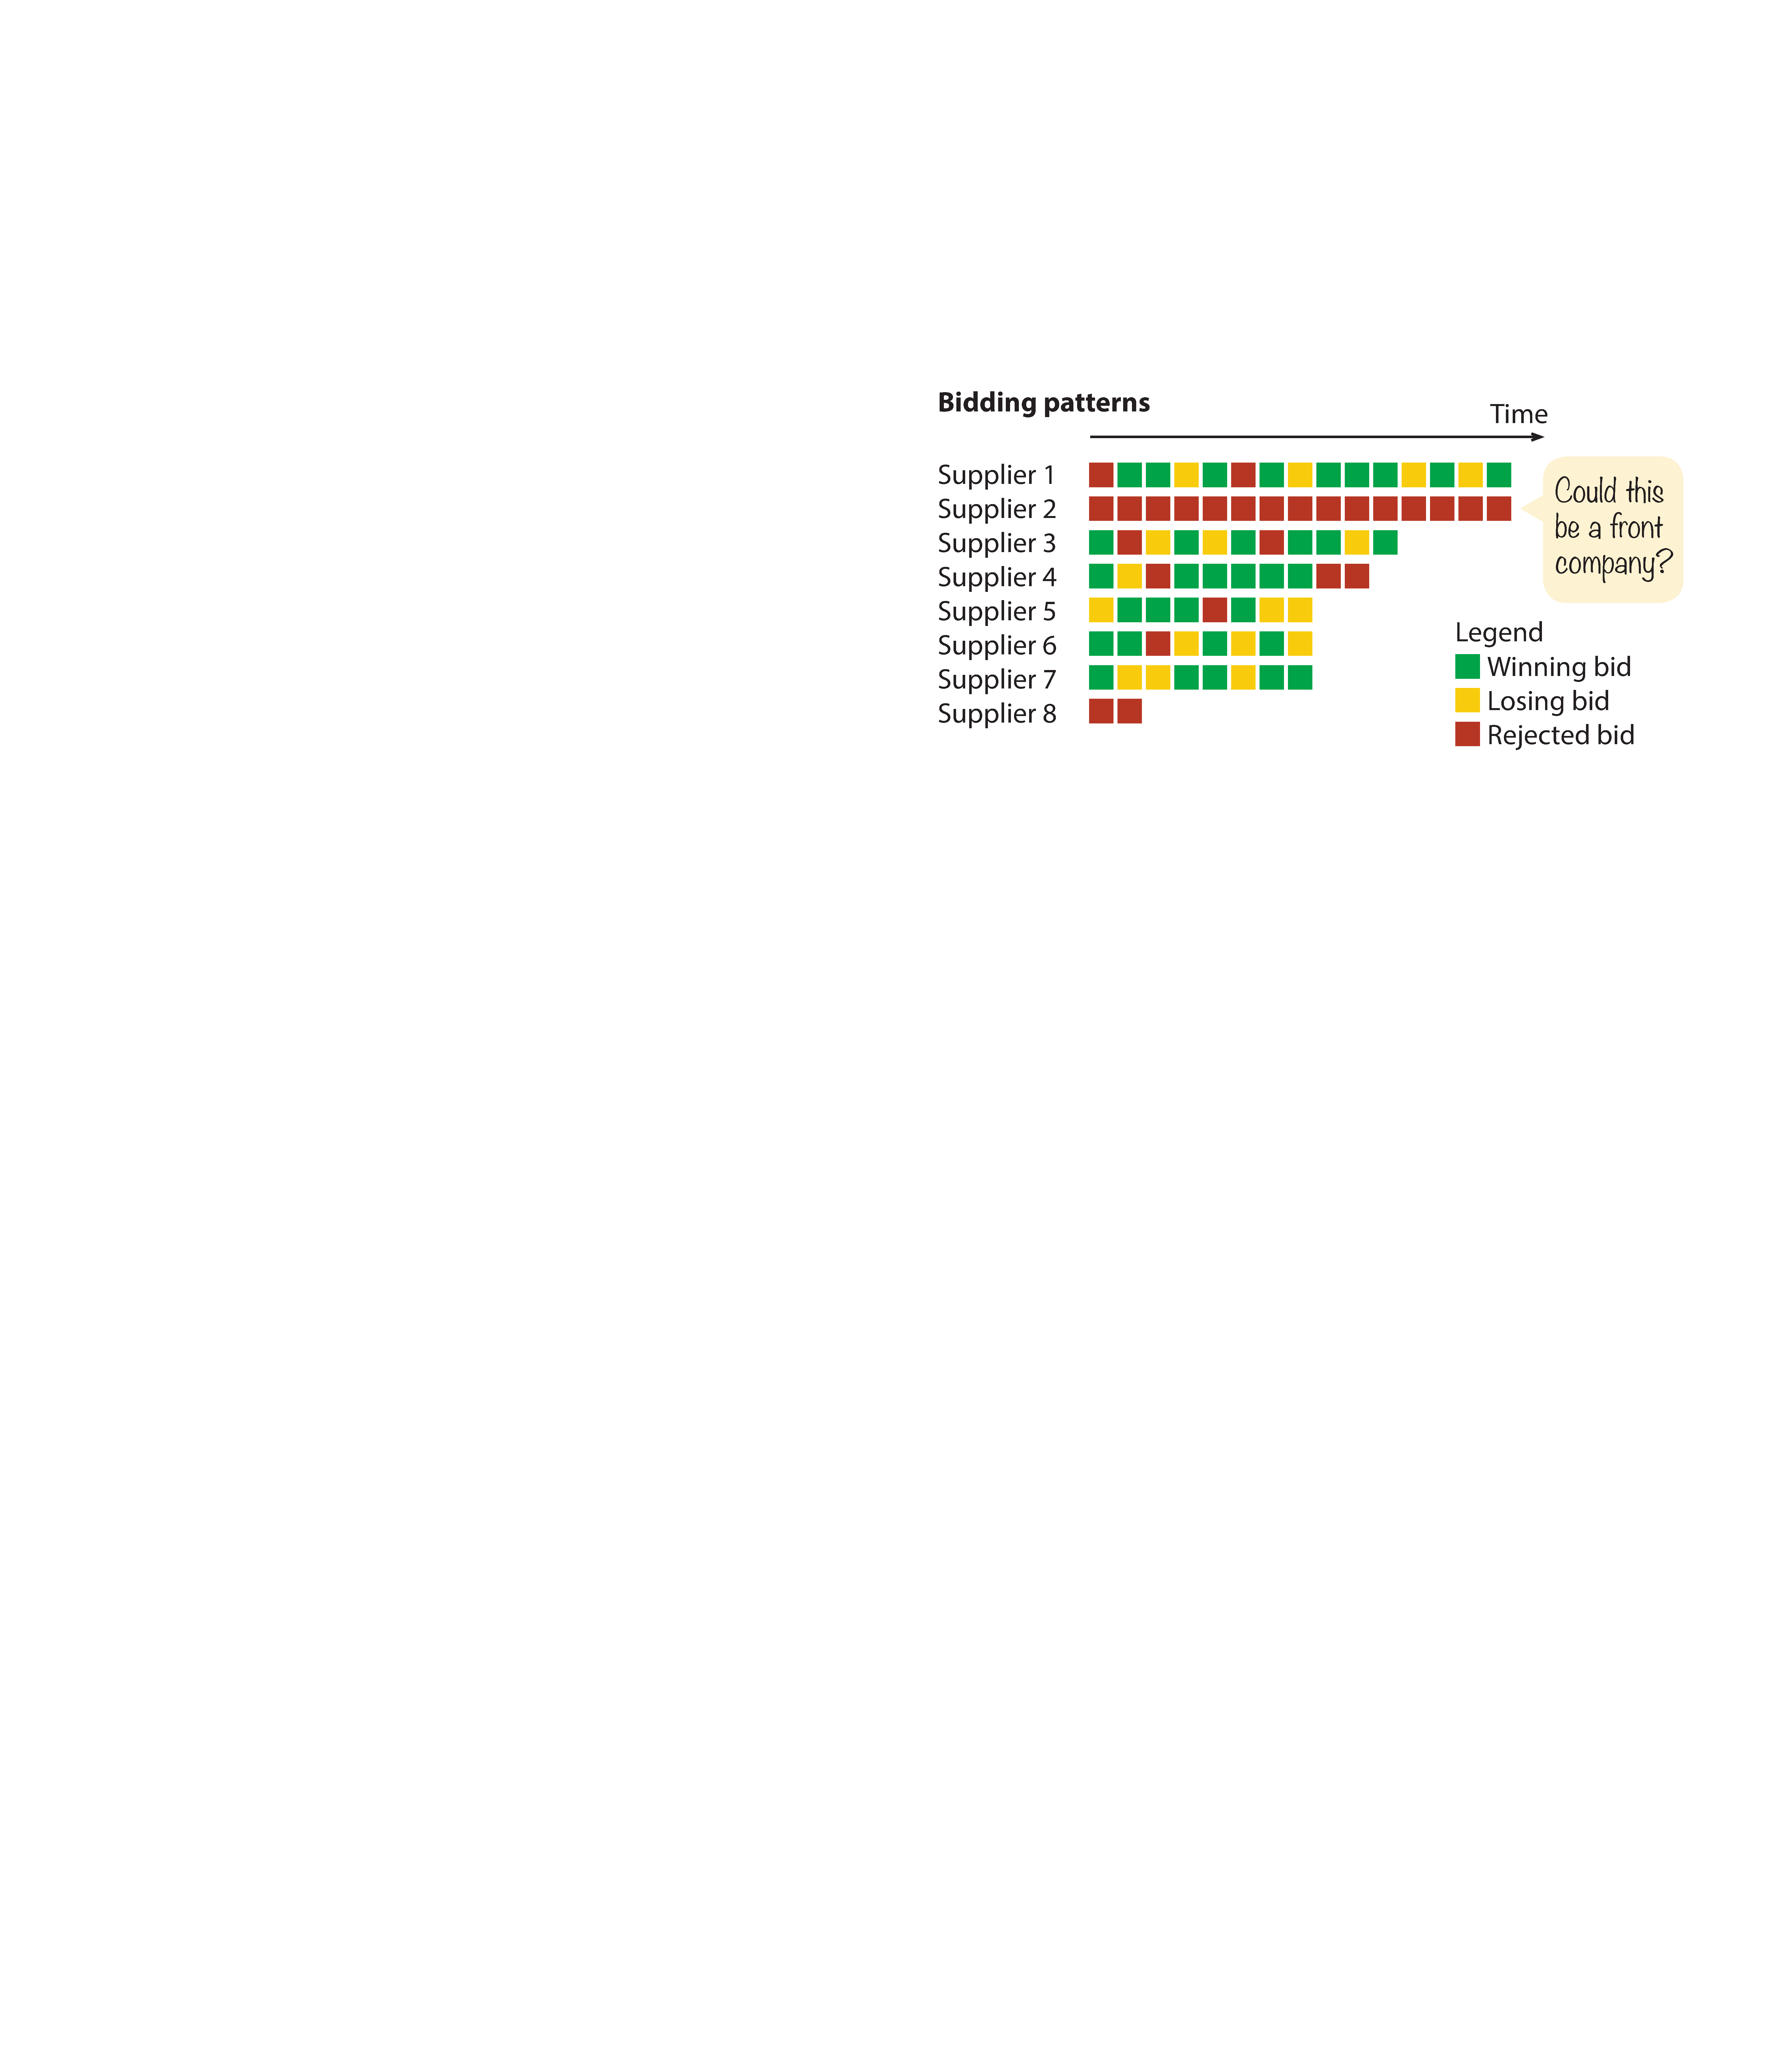
\includegraphics[max width=1\textwidth]{../img/poster_bidding_patt.pdf}
\end{subfigure}

\end{figure}
\clearpage
\begin{figure}[H]
\ContinuedFloat

\begin{subfigure}[t]{0.5\textwidth}
\caption{Participation to call for proposals}
\label{fig_proposals}
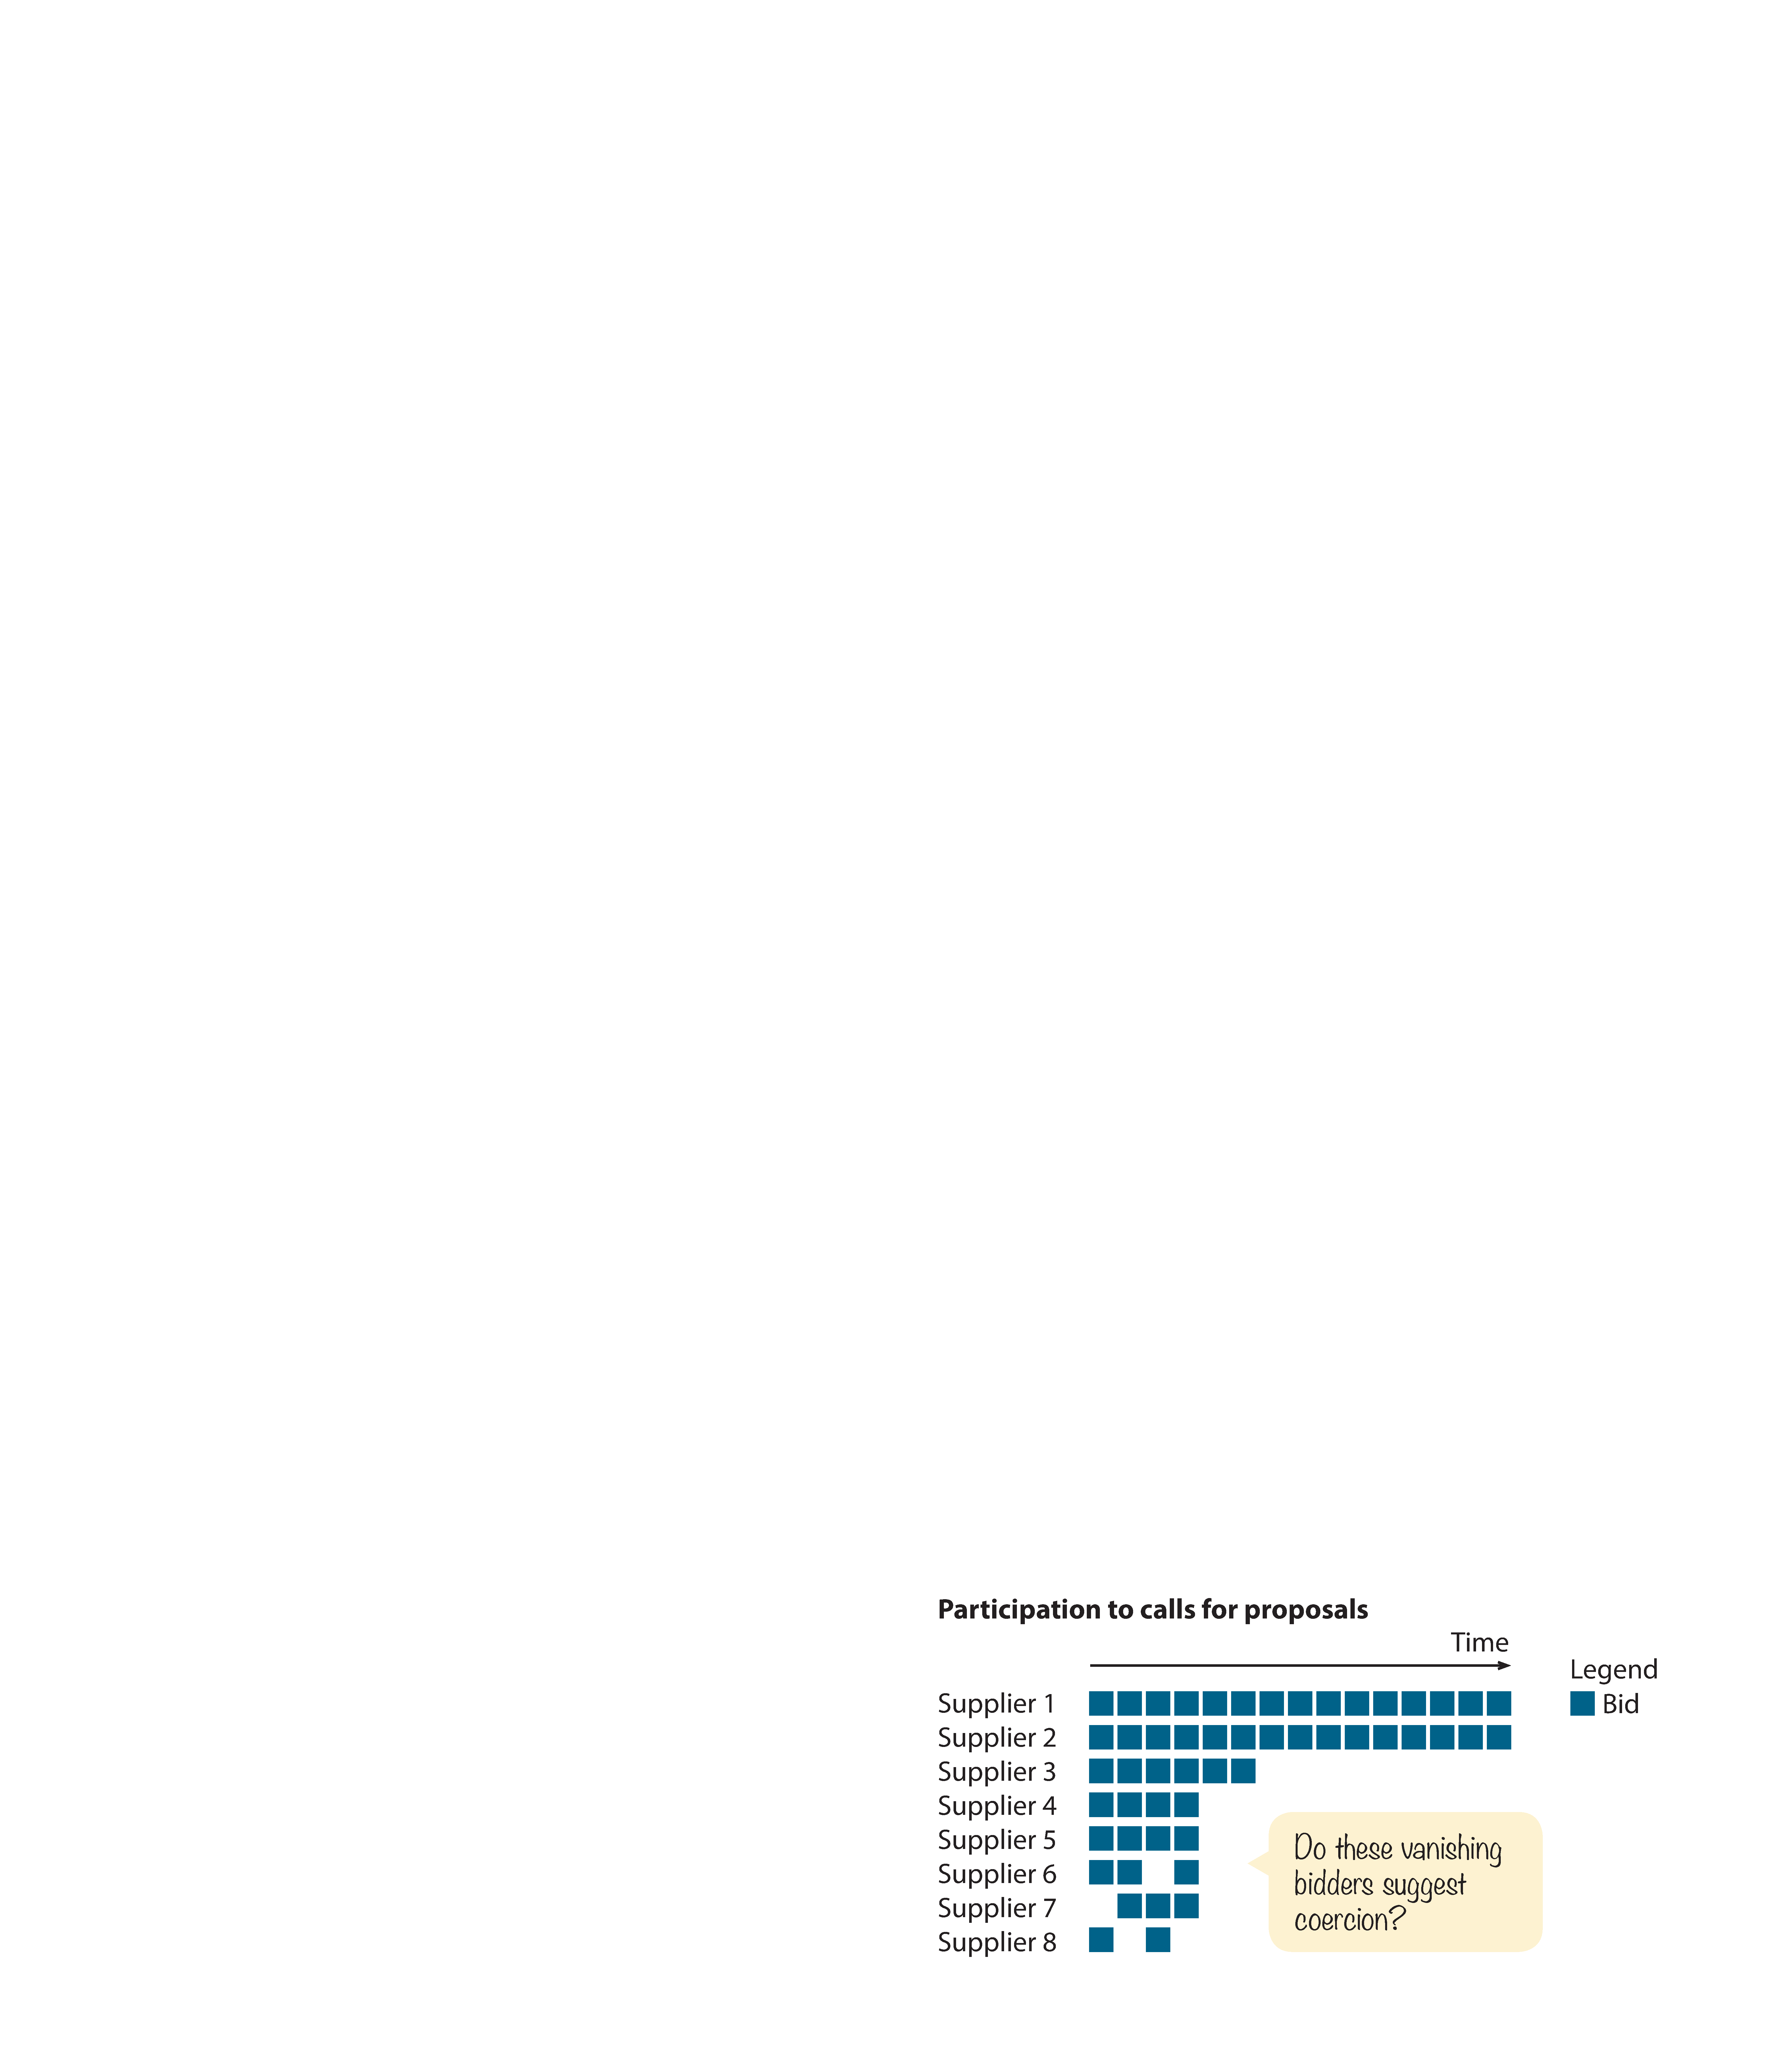
\includegraphics[max width=1\textwidth]{../img/poster_coercion.pdf}
\end{subfigure}
~
\begin{subfigure}[t]{0.5\textwidth}
\caption{Bidding patterns}
\label{fig_bid2}
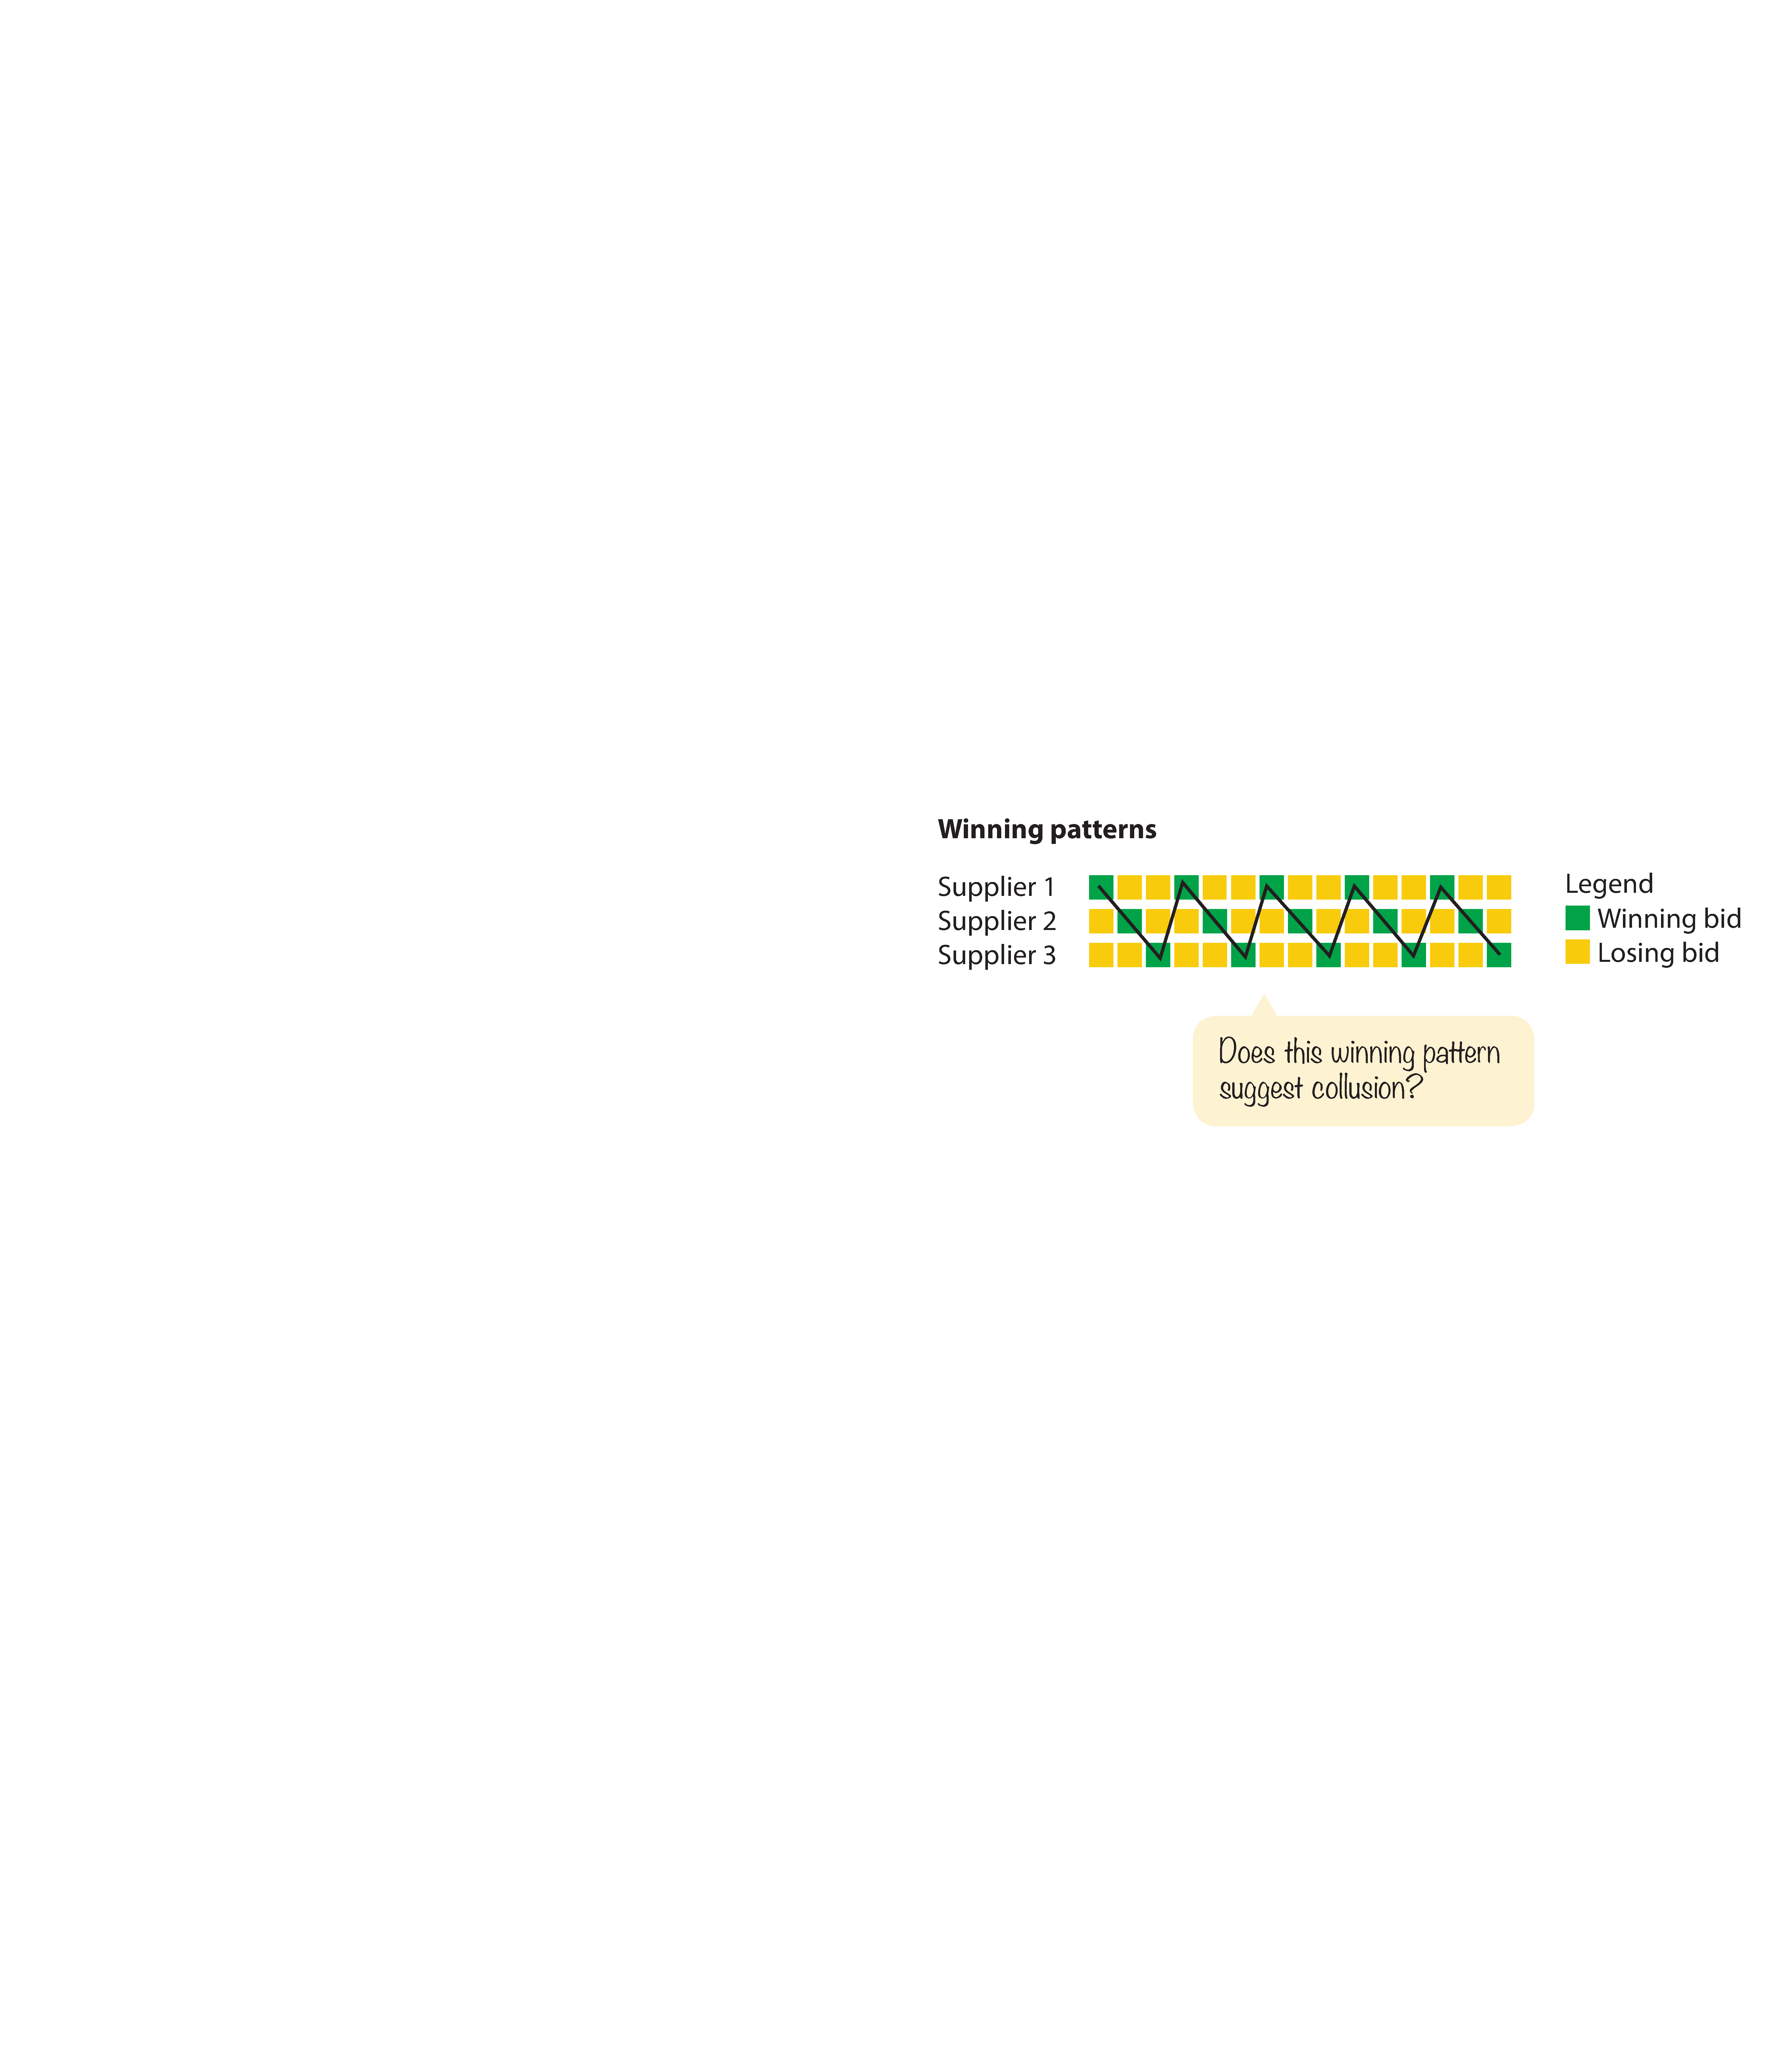
\includegraphics[max width=1\textwidth]{../img/poster_win_pattern.pdf}
\end{subfigure}
\footnotesize{\textbf{Source:} Figures taken from \cite{wb_poster}}
\end{figure}

Another priority during the trip to Washington D.C. was asking questions and learning about the data that will provide a window into the problems that INT is working to address. To data scientists, diving into analysis and model-building right away can be an enticing prospect when presented with an exciting new data set, but engaging with stakeholders and domain experts at the earliest stages can help guide the analysis and save considerable time down the road.








\chapter{The World Bank's Data}\label{chap_data}

As shown on chapter \ref{chap_intro}, collecting the necessary data for any Data Science project is almost always a huge task because the reality tends to be that some of the most relevant variables commonly go unmeasured or are private. This project uses  two types of data, private and public. This chapter describes the two main types of data used for this project.
Section \ref{sec_inv_data} describes the characteristics of private data and the scope it has. It also explains about the confidentiality agreement Integrity Vice Presidency (INT) offered this project in exchange for investigations data. Section \ref{sec_public_data} explains how to download public data from the Wold Bank's servers using coding tools.

\section{Investigations data}\label{sec_inv_data}

The most valuable data for this project was the private data which the partners at INT made available for the project while maintaining a spirit of openness. A confidentiality agreement was signed in order to give access to the investigations database. The only condition was that all the data and analyses had to be stored and processed on a remote server with an encryption and security measurements that satisfied the World Bank's standards. 

In this case the server was an Amazon Web Service's (AWS), Amazon Elastic Compute Cloud (Amazon EC2) machine. EC2 is a web service that provides resizable compute capacity in the cloud. It is designed to make web scale cloud computing easier for developers\footnote{``Amazon EC2’s simple web service interface allows you to obtain and configure capacity with minimal friction. It provides you with complete control of your computing resources and lets you run on Amazon’s proven computing environment. Amazon EC2 reduces the time required to obtain and boot new server instances to minutes, allowing you to quickly scale capacity, both up and down, as your computing requirements change. Amazon EC2 changes the economics of computing by allowing you to pay only for capacity that you actually use. Amazon EC2 provides developers the tools to build failure resilient applications and isolate themselves from common failure scenarios.'' \parencite{aws_es2}}. For more details on how to setup an AWS computer see \parencite{aws_start} and appendix \ref{chap_software}. In other words, the data was stored in an AWS machine on the cloud that had an encrypted folder with the specific files. Since all the data had to stay on the cloud, all the processing had to be done on the cloud too. For this purpose, a server running \texttt{Python} and \texttt{R} was hosted at an AWS computer. 


\subsection{Basic description}

The investigations data consists of nearly 13,000 cases, of which over half are Fraud and Corruption. 377 are labeled as Collusion. These are from the ``Allegation Category'' column, Notably, allegation categories include Fraud, Corruption, and Fraud \& Corruption. It is possible for a case's description to just say Fraud and for its allegation category to still be Fraud and Corruption. I would suggest treating each of these 3 categories as the same (i.e. all ``Fraud and Corruption'').

Allegations also include a ``Allegation Sub-Category''. Collusion is sometimes listed as a sub-category, for example: Allegation Category: Fraud and Corruption or Allegation Sub-Category: Bid Manipulation/Collusion.

The Unit of analysis is the investigations data is the ``Subject'' column. Mostly this variable refers to companies and people, but on occasion other entities on a project may be subjects of investigation, for example the coordinating agency. For example Case \# C-EGT-2010-1754, the subject is: Egyptian Ministry of Education. In procurement data it shows up in ``Implementing Agency'' column as: \texttt{PPMU-MINISTRY OF EDUCATION}
    
The Labels in the investigations are very different and specific to each investigation case. The most relevant label will be the Allegation Outcome's column. The most frequent outcomes for a case are ``Substantiated'', which means that the Subject was found to be guilty of the Allegation, ``Unfounded'', which means that the Subject was found to be  innocent of the allegation, and ``Unsubstantiated'', which means that the investigation did not have the necessary means to conclude that the subject was  guilty, but neither does it have to conclude that the subject is innocent. Substantiated and Unsubstantiated occur in roughly equal quantities, while Unfounded is fairly rare. There are other, rarer labels, like ``We kicked it to another organization''.

The identities of the cases within the investigations data include that about 80\% of the data has either the name of the accused (the majority) or the project number (about a third). These are in the Subject and Project Number columns, respectively. That means about 20\% of the data appears to be ``lost'', in that we can't match it up to any procurement data. There is potentially other information in the ``Title'' field, but it is unstructured. There could theoretically be information in other fields, but they are not as rich.

There are among 1000 different sectors but most of them are mixed sectors and have not been previously cleaned. For example, when an investigation involves cases that cover sectors such as transportation and urban development there can be the case that you find a Transportation sector, a Urban Development sector and a Transportation \& Urban Development Sector. For the specifics of the model, this project works with sector specific as they are, this meaning that, for the project, the three cases mentioned before are considered to be different sectors. By doing so, there are about 205 sectors.

% Questions [for Betsy?]
% ==
% - What's the difference between 'Allegation Outcome' and 'Outcome of Overall Investigation When Closed', because these often give different outcomes (Substantiated, Unsubstantiated) (Outcomes different: 10422, Outcomes same: 2301)
% - In sector names, what's the difference between "Transportation" and "SDN - Transport"
%  - Ditto "Energy/Mining" and "SDN - Energy/Mining"





\section{Public data}\label{sec_public_data}


Fortunately for the project, not all the data was private. This work uses the Open Data\footnote{Go to \cite{wb_data}.}  and the Data Bank websites from the World Bank, which offer free access to comprehensive, downloadable indicators about development in countries around the globe. 

Public data from the World bank comes from different databases. They are generated at different sections within the World Bank so each indicator can be obtained form a specific database according to its nature. For example, all the Development indicators can be obtained at the World Bank's World Development Indicators database, indicators regarding how easy it ts to do business in each specific country could be obtained from the Doing Business database and indications regarding world's populations can be obtained at the Health Nutrition and Population Statistics database.\footnote{Different databases include:
Africa Development Indicators, Statistical Capacity Indicators, Country Policy and Institutional Assessment (CPIA), Country Partnership Strategy for India, Corporate Scorecard, Doing Business, Exporter Dynamics Database: Country-Year, Education Statistics, Enterprise Surveys, Global Findex ( Global Financial Inclusion database), G20 Basic Set of Financial Inclusion Indicators, Gender Statistics, Global Economic Monitor, GEP Economic Prospects, Global Financial Development, Global Economic Monitor (GEM) Commodities, Global Partnership for Education, Global Social Protection, Health Nutrition and Population Statistics, Health Nutrition and Population Statistics by Wealth Quintile, Health Nutrition and Population Statistics: Population estimates and projections, International Development Association - Results Measurement System, INDO-DAPOER, International Debt Statistics, Jobs for Knowledge Platform, LAC Equity Lab, Millennium Development Goals, Povstats, Quarterly Public Sector Debt, Quarterly External Debt Statistics/GDDS (New), Quarterly External Debt Statistics/SDDS (New), Readiness for Investment in Sustainable Energy (RISE), Sustainable Energy for All, Subnational Malnutrition Database, Subnational Poverty, Subnational Population, Wealth accounting, World Development Indicators and the  Worldwide Governance Indicators.}

A good practice in Data Science is to generate code so that all results can be easily replicated. That was the reason why, for this project all the data that the World Bank bank provides publicly by an Application Programming Interface (API) was collected with reliable code. Thanks to prior World Bank's work, accessing the World Bank Data APIs with code in languages such as \texttt{Python}, \texttt{R}, \texttt{Ruby} and \texttt{Stata} is a simple task. The World Bank has a blog where they explain in detail how to use the APIs. See the \cite{wb_api}, the \cite{wb_python} and the \cite{wb_r} for more details on how to do this. To put things in context, \texttt{Python} and \texttt{Ruby} are general-purpose programming languages, and \texttt{Stata} and \texttt{R} are programming environments optimized for statistics. They're all widely used in the business and academic worlds. The World Bank generates modules to those languages which help users to connect to the World Bank Development Indicators API and access the latest data.

For example, in \texttt{python}, the \texttt{wbdata} module by Oliver Sherouse offers easy access to all the data in the World Bank's APIs. It also plays nicely with Wes McKinney’s  \texttt{pandas} analysis library\footnote{See appendix \ref{chap_software} for \texttt{pandas} details.}. \texttt{Wbdata} is a simple python interface to find and request information from the World Bank's various databases, either as a dictionary containing full meta data or as a \texttt{pandas} Data Frame. Currently, \texttt{wbdata} wraps most of the World Bank API, and also adds some convenience functions for searching and retrieving information.

In \texttt{R}, the \texttt{WDI} module by Vincent Arel-Bundock offers convenient access to the data in the World Bank's API. For fast searching, the \texttt{WDI} package ships with a local list of available data series. This local list can be updated to the latest version using the \texttt{WDIcache} function \parencite{wb_r}. Similar tools are available to languages such as Ruby and Stata.

Given that, the public data used in this project can be divided in two sets; first, the World Bank's World Development Indicators, which can be obtained by using the API and the packages mentioned; and, second, all the historical and major awards given by the World Bank to all developing countries from 1990 to 2014. 


\subsection{World Development Indicators}

The World Bank has a major data base called: World Development Indicators (WDI). WDI is the primary World Bank collection of development indicators, compiled from officially recognized international sources. This database represents the most current and accurate global development data available, and includes national, regional and global estimates. For the purpose of this work, the indicators selected such that prediction of corruption, collusion and fraud would not be attainable to specific country variables such as country or country region. This is was because the World Bank can not start investigation cases in specific countries just because different countries tend to have different levels of corruption. Unfortunately, those types of variables can have, in some times, much better prediction rates but the policies at the World Bank prevents a model of having them for discretion and discrimination arguments.

Also, the World Bank has around 16,000 different indicators the project could use, but being this big, and according to purpose of this project, only a few indicators were selected. The next list shows the ones that were considered. This list includes indicators related to the private sector and trade among countries which is the theme the project is targeting.

\begin{description}
\item[IC.BUS.DISC.XQ]	Private Sector \& Trade: Business environment. Business extent of disclosure index (0=less disclosure to 10=more disclosure)	Disclosure index measures the extent to which investors are protected through disclosure of ownership and financial information. The index ranges from 0 to 10, with higher values indicating more disclosure.
\item[IC.FRM.CMPU.ZS]	Private Sector \& Trade: Business environment. Firms competing against unregistered firms (\% of firms).
\item[IC.FRM.CORR.ZS]	Private Sector \& Trade: Business environment	Informal payments to public officials (\% of firms).
\item[IC.FRM.INFM.ZS]	Private Sector \& Trade: Business environment	Firms that do not report all sales for tax purposes (\% of firms).
\item[IC.LGL.CRED.XQ]	Private Sector \& Trade: Business environment	Strength of legal rights index (0=weak to 10=strong).
\item[IC.LGL.DURS]	Private Sector \& Trade: Business environment	Time required to enforce a contract (days).
\item[IC.TAX.GIFT.ZS]	Private Sector \& Trade: Business environment	Firms expected to give gifts in meetings with tax officials (\% of firms).
\item[IQ.CPA.PROP.XQ]	Public Sector: Policy \& institutions	CPIA property rights and rule-based governance rating (1=low to 6=high).
\item[IQ.CPA.TRAN.XQ]	Public Sector: Policy \& institutions	CPIA transparency, accountability, and corruption in the public sector rating (1=low to 6=high).
\item[NY.GDP.PCAP.CD]	Economic Policy \& Debt: National accounts: USD at current prices: Aggregate indicators	GDP per capita (current US\$).
\item[SE.PRM.PRSL.ZS]	Education: Efficiency	Persistence to last grade of primary, total (\% of cohort).
\item[SI.POV.GINI]	Poverty: Income distribution GINI index.
\item[SL.UEM.TOTL.NE.ZS]	Social Protection \& Labor: Unemployment	Unemployment, total (\% of total labor force) (national estimate).
\end{description}

The code to download WDI can be seen at the Appendix \ref{chap_code} in code \ref{code_wdi}. This code can easily replicate results. For the purpose of this work, the code in \ref{code_wdi} downloads data for the countries within the countries from the investigations data, those countries define the countries list for this work.



\begin{figure}[H]
\begin{center}
\caption{WDI: \% of Bribes to tax officials per Country/Region}
\label{fig_wdi_bribes}
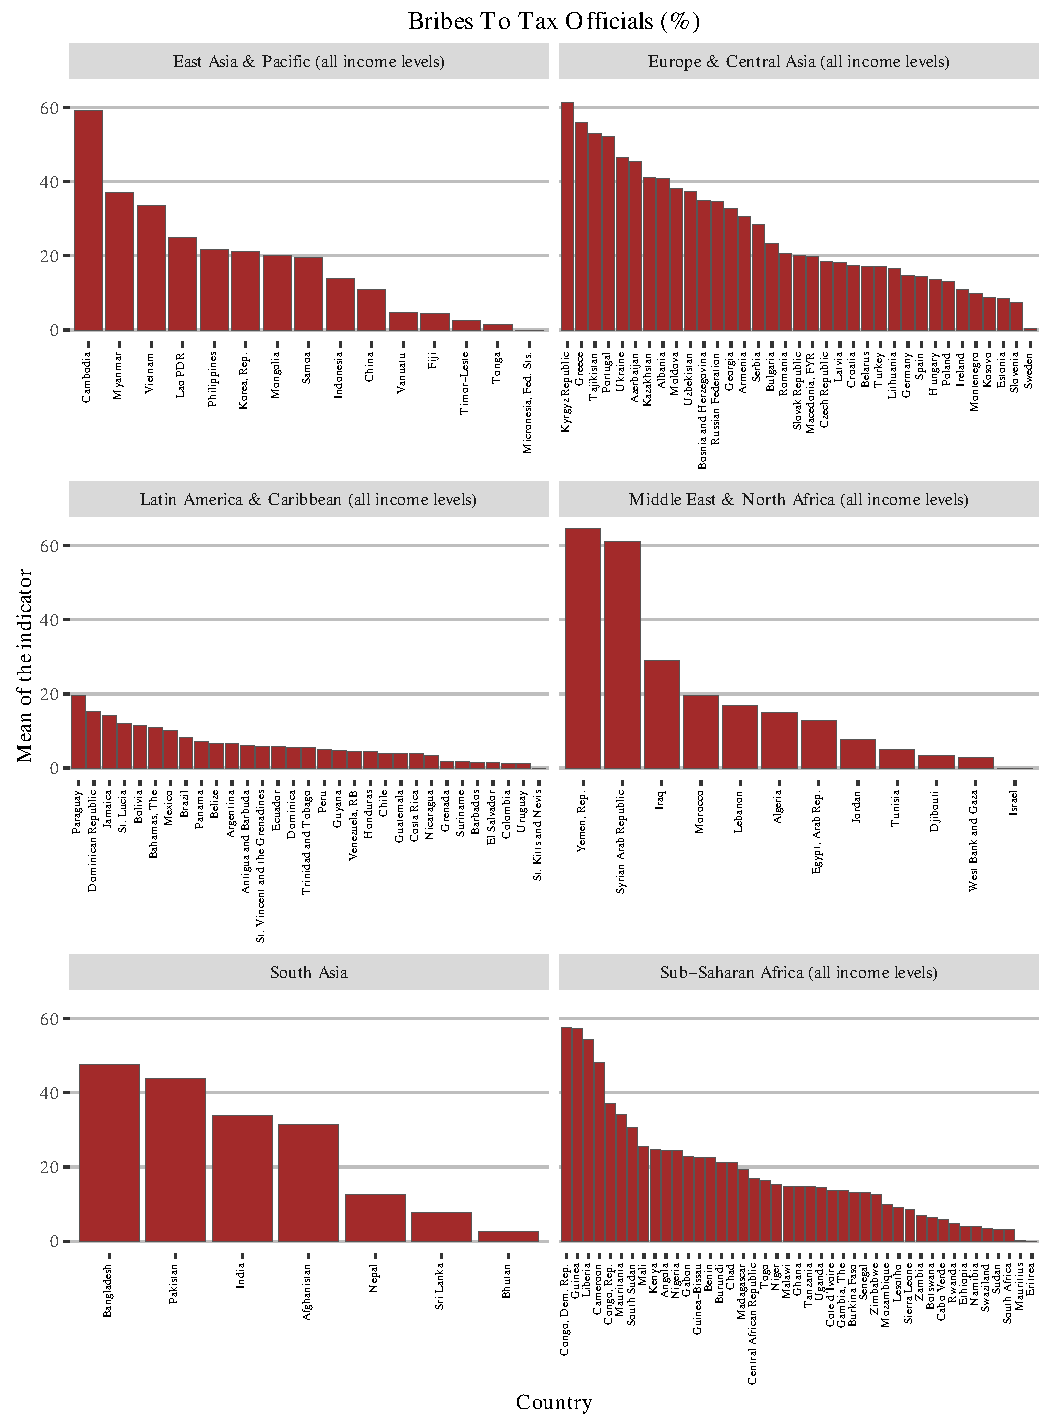
\includegraphics[max height=.9\textheight]{../img/wdi_bribes_to_tax_officials_perc.pdf}
\end{center}
\noindent \footnotesize{\textbf{Source:} Own creation and data obtained with package \texttt{WDI}, see the \cite{wb_r}.}
\end{figure}

\begin{figure}[H]
\begin{center}
\caption{WDI: \% of Firms competing against informal firms per country/Region}
\label{fig_wdi_firms}
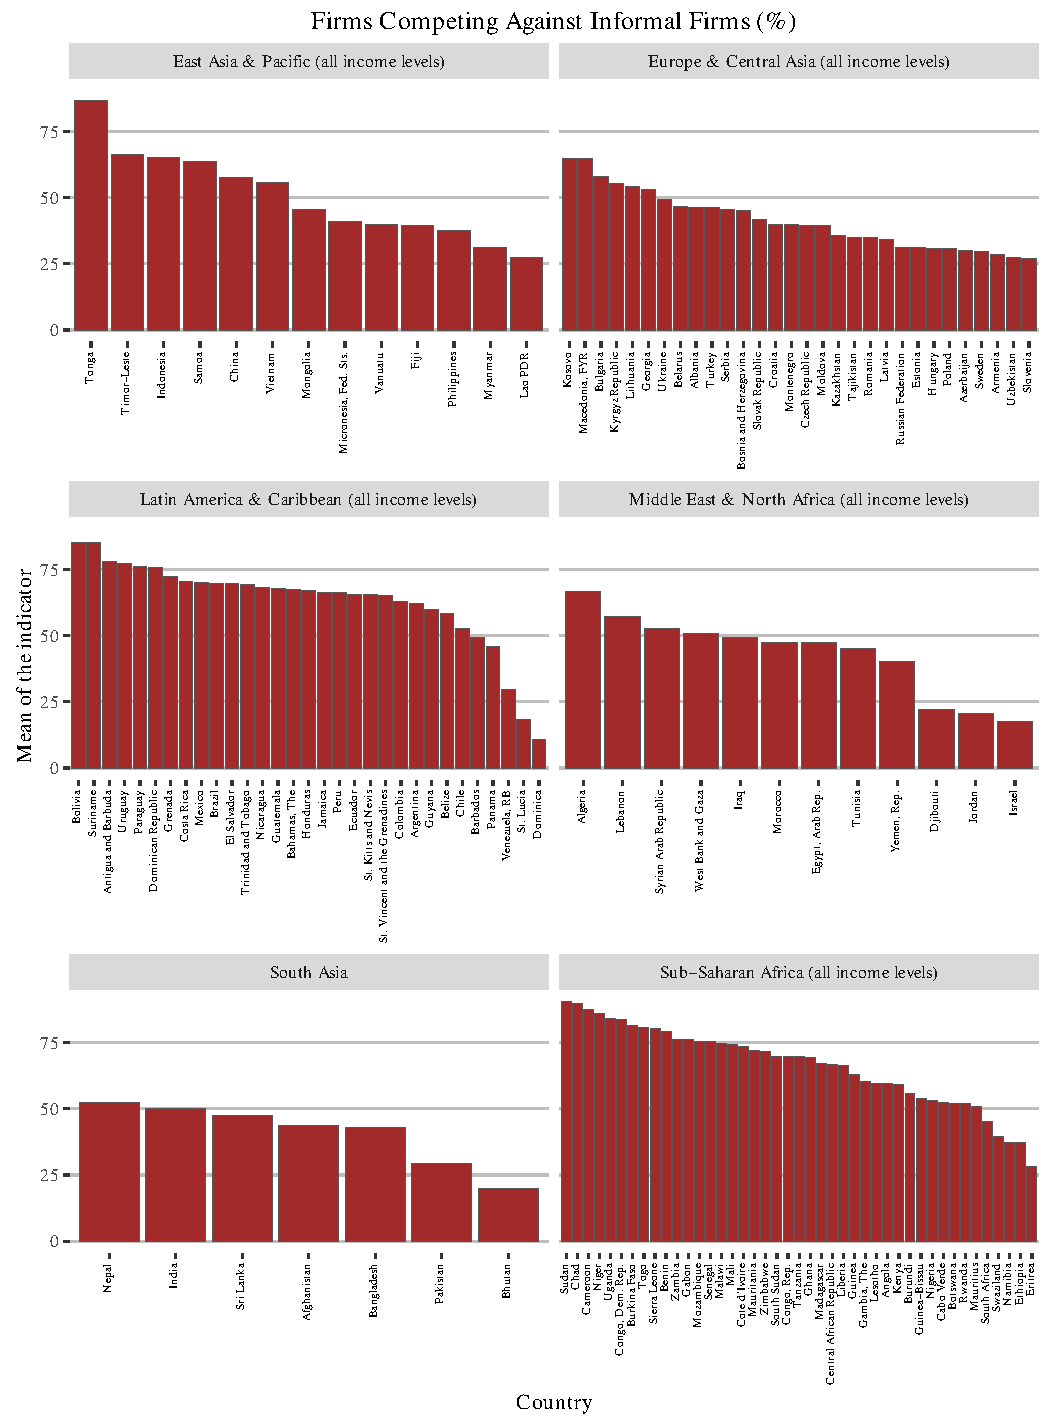
\includegraphics[max height=.9\textheight]{../img/wdi_firms_competing_against_informal_firms_perc.pdf}
\end{center}
\noindent \footnotesize{\textbf{Source:} Own creation and data obtained with package \texttt{WDI}, see the \cite{wb_r}.}
\end{figure}

\begin{figure}[H]
\begin{center}
\caption{WDI: \% of Payments to public officials per Country/Region}
\label{fig_wdi_pays}
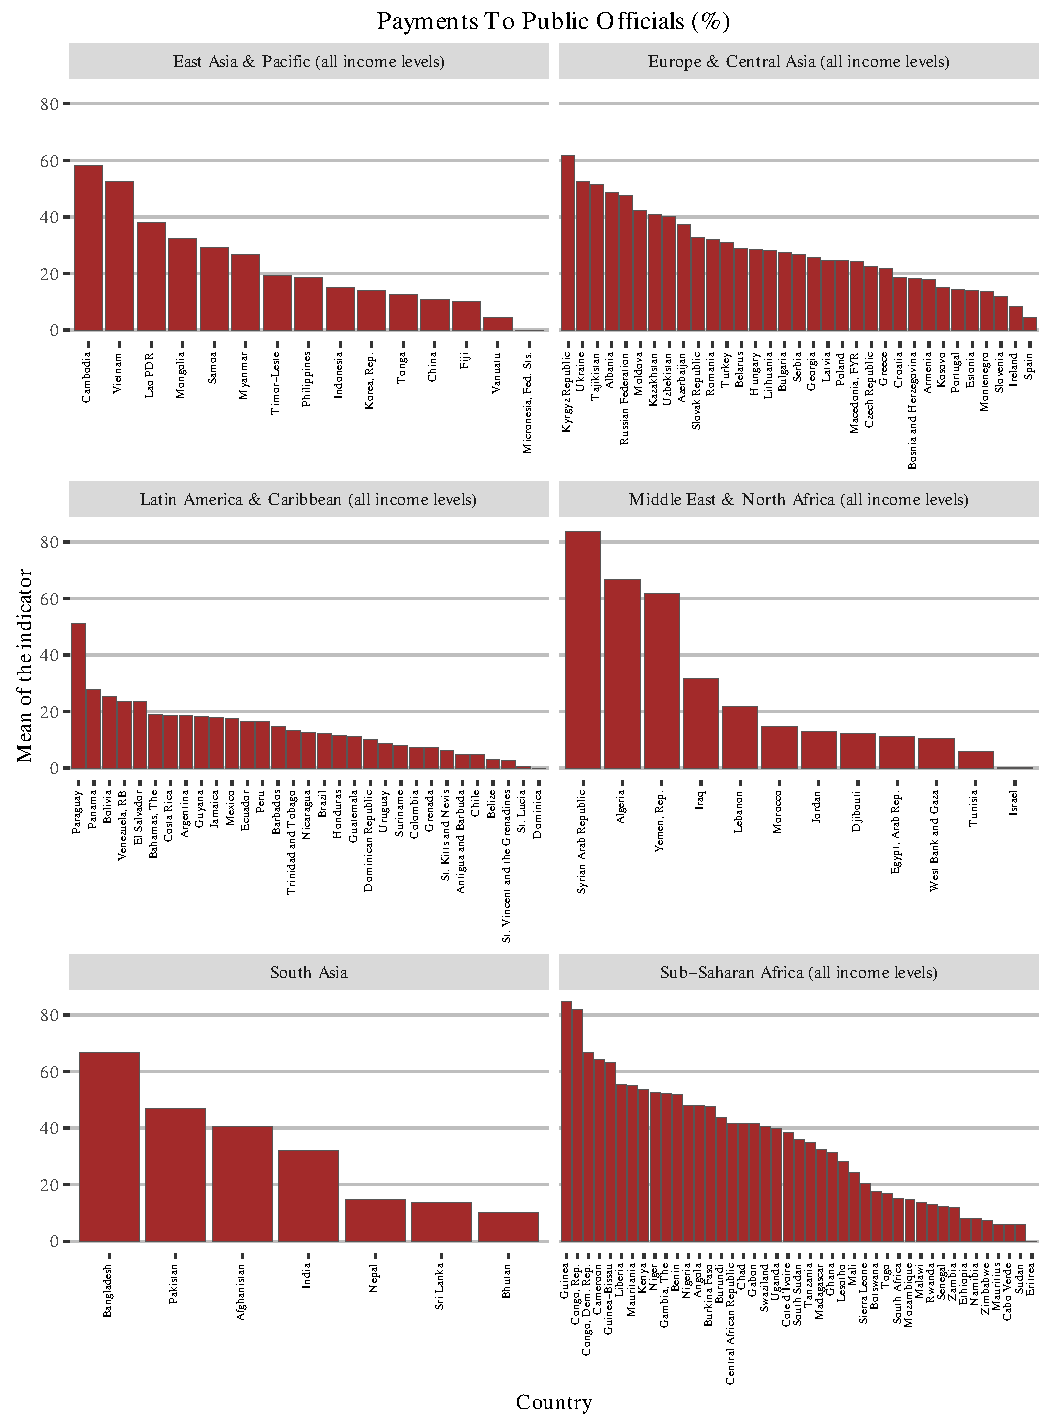
\includegraphics[max height=.9\textheight]{../img/wdi_payments_to_public_officials_perc.pdf}
\end{center}
\noindent \footnotesize{\textbf{Source:} Own creation and data obtained with package \texttt{WDI}, see the \cite{wb_r}.}
\end{figure}


\begin{figure}[H]
\begin{center}
\caption{WDI: Time to Enforce Contracts per Country/Region}
\label{fig_wdi_time_contract}
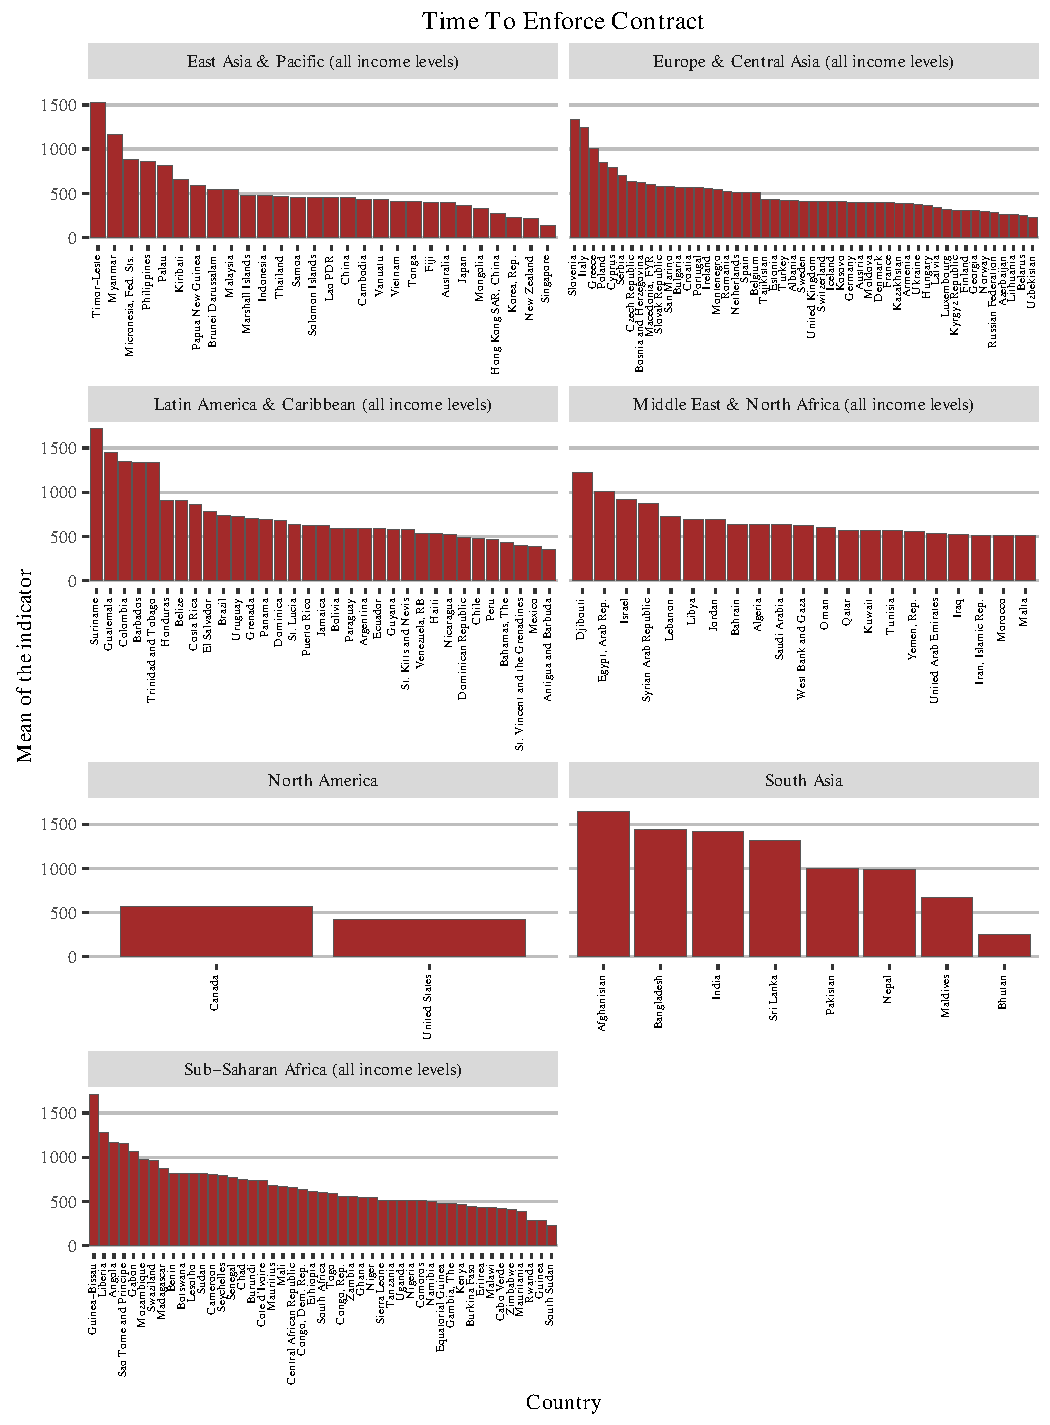
\includegraphics[max height=.9\textheight]{../img/wdi_time_to_enforce_contract.pdf}
\end{center}
\noindent \footnotesize{\textbf{Source:} Own creation and data obtained with package \texttt{WDI}, see the \cite{wb_r}.}
\end{figure}


\subsection{Major and Historic Awards}



\section{Disambiguation}

% \input{B4_theoretical.tex}

\chapter{Detecting corruption, collusion \& fraud: Data product}\label{chap_product}


This chapter first describes the details in the modeling process for the identification of possible cases of corruption, collusion and fraud within the World Bank's Major and Historical awards and investigations data. After that, this chapter explains  how does the visualization created for the World Bank's investigation team in the Integrity Vice Presidency works. Section \ref{sec_pipeline} is a visualization of the data pipeline that sustains the web application that runs in the Wolrd Bank's servers. Section \ref{sec_models} gives the details of the model selected for the identification of corruption, collusion and fraud and finally, section \ref{sec_visual} shows the different visualizations made for a more proactive investigation process.

\section{Data pipeline} \label{sec_pipeline}

As chapter \ref{chap_data} shows, there are different data sources, figure \ref{fig_pipeline} shows a summary of how the data from all the sources was combined into a web application that runs in the server of the World Bank and helps the investigators at the Integrity Vice Presidency to investigate projects and entities in a more proactive way than by relying on whistle-blowers. Figure \ref{fig_pipeline} shows how the different data sources first combine into the Google Algorithm for name disambiguation explained on chapter \ref{chap_data}. Then the resulting tables are joined with the World Bank's Development indicators for each country. After this, all the country specific and co-award network features explained in section \ref{sec_features} were produced so that finally everything feeds the model that can potentially identify malicious contracts or contractors.

\begin{figure}[H]
\begin{center}
\caption{Data pipeline}
\label{fig_pipeline}
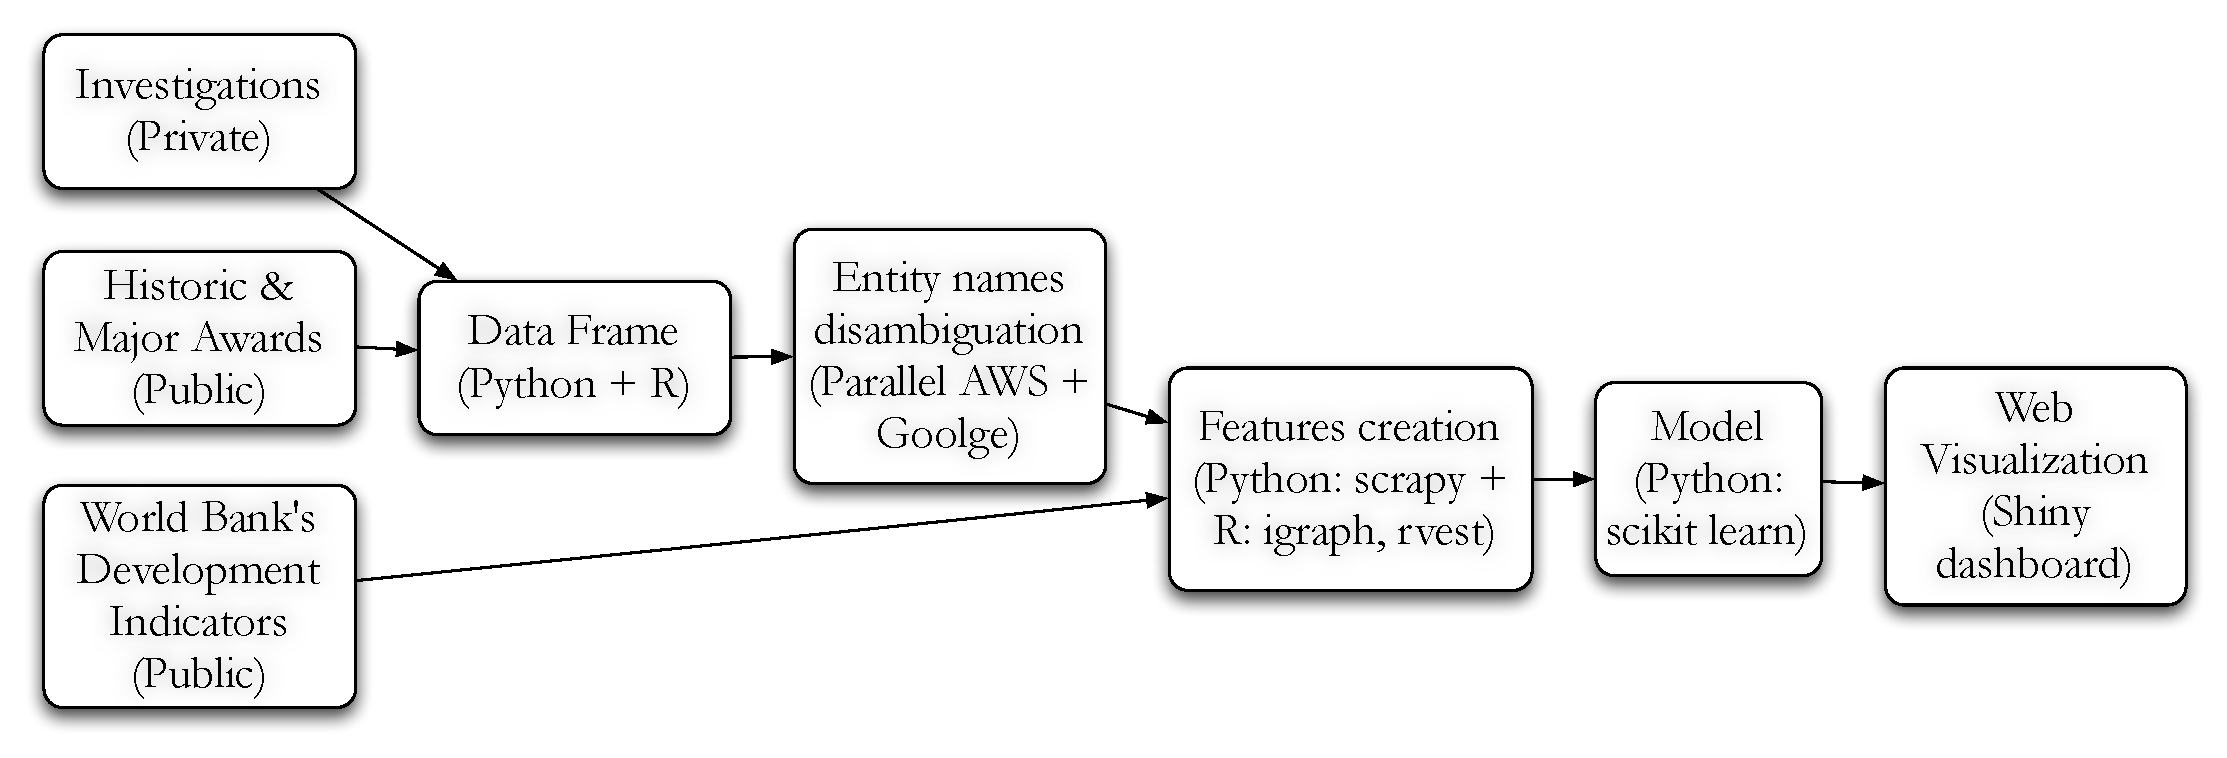
\includegraphics[width=\textwidth,height=1\textheight,keepaspectratio]{../img/pipeline.pdf}
\end{center}
\noindent \footnotesize{\textbf{Source:} Own creation.}
\end{figure}

The steps illustrated  in figure \ref{fig_pipeline} were explained in previous chapters up to the feature creation. The next sections cover the modeling and the visualizations.

\section{Model} \label{sec_models}

As the introduction says in page \pageref{dssg} any Data Science project such as this one requires a solvable problem, that is challenging, has impact, has relevant data and a committed partner. Up to this face we have stated that detecting corruption, collusion and fraud  is challenging enough, the Google searches algorithm and the co-awards network is a clear example of that. The impact was stated in figures such as \ref{fig_major_awarded_usd} that shows the amount that the World Bank gives in its procurements contracts in its effort to reduce global poverty. This project has relevant data  from different sources that complement to each other and a clearly committed partner. So, up to this point the project is just missing a solution to the identification of corruption, collusion and fraud such that it becomes a solvable problem.  

We needed to create a solvable problem within the time restrictions stated at the time of the project. Unfortunately, the most relevant data came way after the project started and the name disambiguation algorithm took long enough to have  enough time for the next steps of the project, which was, the modeling step. The idea was to find a model that is able to identify potential cases of corruption, collusion or fraud within the World Bank's data. 

A traditional modeling process like this involves comparing different approaches in order to minimize the desired error or maximize the accuracy of a classification or prediction.


For this project, three different models were considered, a classifier  using a Supported Vector Machine (SVM), a Random Forest and a Logistic Regression. To evaluate the output we created the dependent variable by considering the labels in the investigations data by labeling any substantiated case as guilty and not guilty in any other case. See \cite{hasti} for more details on SVM, random forest and logistic regression. 


To select the models we first took a training set from the data by sorting it by date so that the data for the past would be able to identify potential corruption, collusion and fraud in the data for the future relative to the training data. To select the parameters of each model we used some crossed validation in terms of the Area Under Curve (AUC) of the Receiver Operating Characteristic curve (ROC), ROC-AUC. See \ref{chap_code} and the code \ref{code_models} to see how the parameters of the models were selected.

Since all the investigations data was private, unfortunately for this paper,  the modeling phase cannot be replicated because of the access to the data so the paper cannot show the results of the different models tunned. Nevertheless, after tunning with different parameters and considering different features, the resulting model was a Random Forest which has a ROC curve that can be seen at figure \ref{fig_roc}. The figure \ref{fig_roc} contains the percentage of the  investigated and not guilty contracts that were marked  by the model as ``should be investigated'' (false positive rate) against the percentage of investigated contracts caught by the model (true positive rate).The figure shows in green the ROC curve for the random forest considering the co-awards network features and the blue curve refers to the ROC without the co-awards network features. As it can be seen from the figure, the network features add accuracy to the prediction so they are very desirable for the World Bank Investigators.

It is also important to notice here that the random forest is a great model for the investigators at the Integrity Vice Presidency because it is a much better classifier than the actual benchmark which was just guessing whether they should investigate a contract, entity or project or not. The dashed line in figure \ref{fig_roc} represents a random guess, so the farther the ROC curve is from that line, the better the quality of the classification.

\begin{figure}[H]
\begin{center}
\caption{ROC: Random forest test data}
\label{fig_roc}
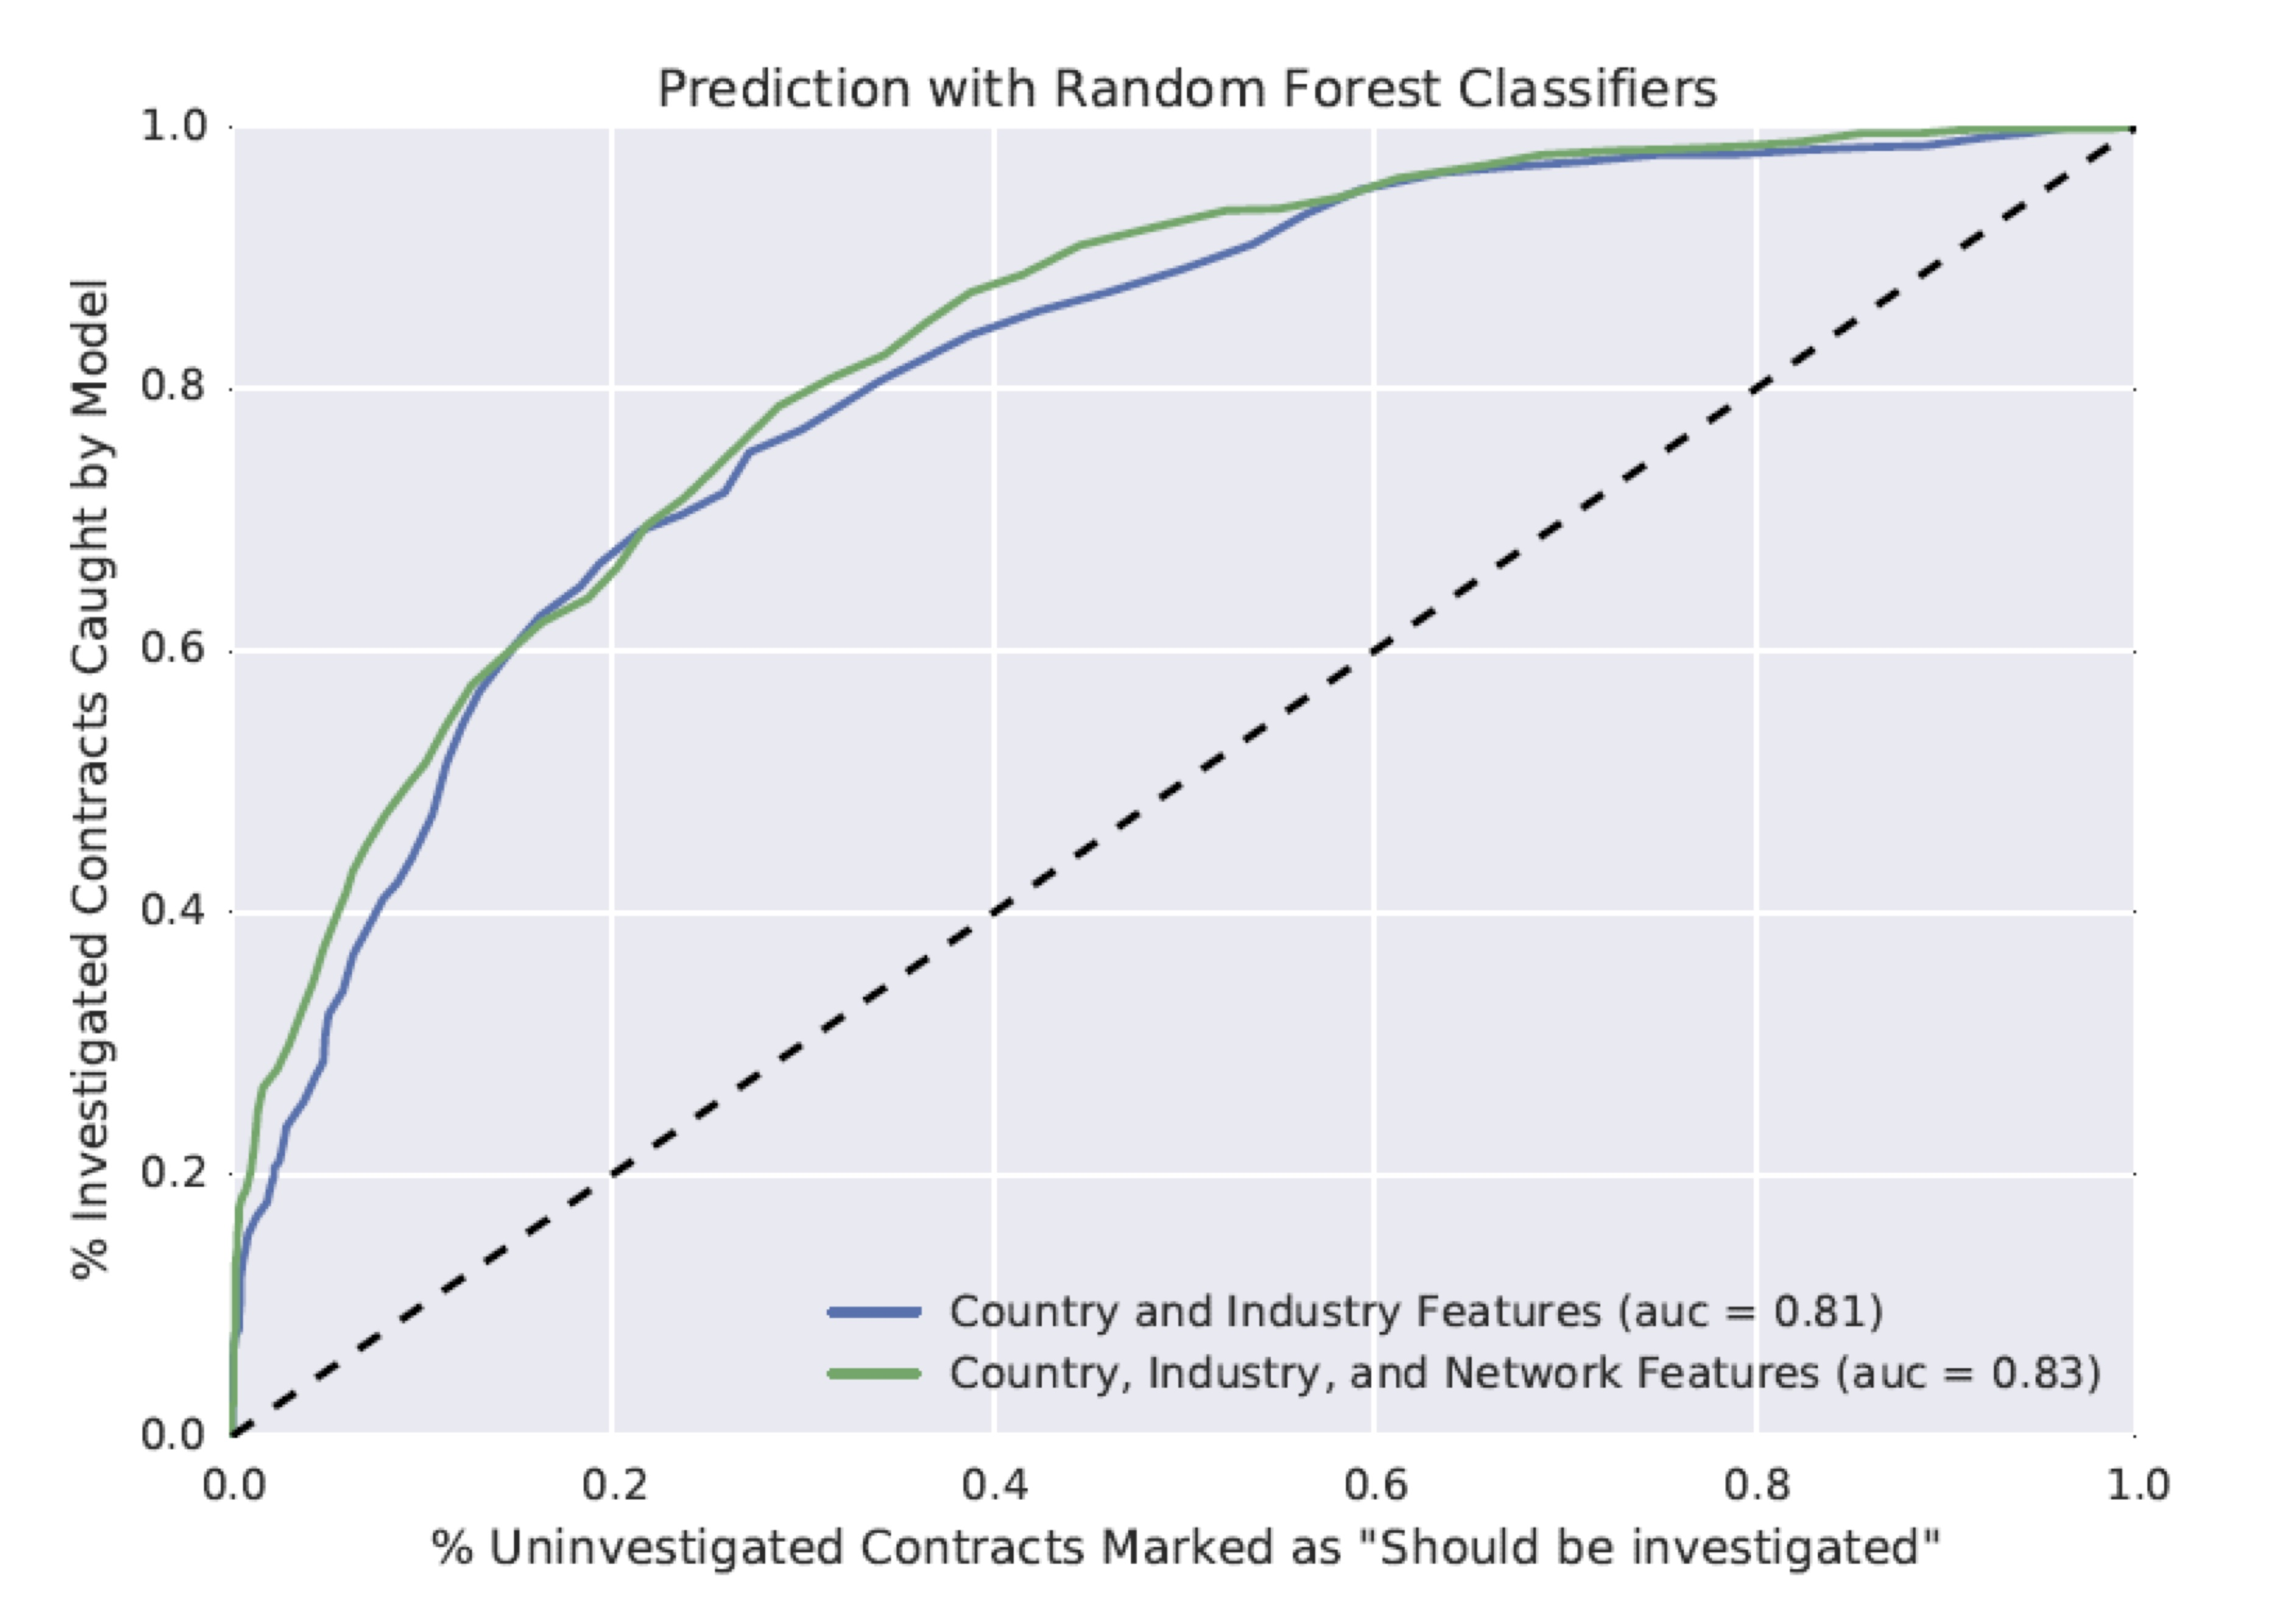
\includegraphics[width=1.05\textwidth,keepaspectratio]{../img/roc.jpg}
\end{center}
\noindent \footnotesize{\textbf{Source:} Own creation.}
\end{figure}


\section{Web visualization application: dashboard} \label{sec_visual}

In order for the investigators at the World Bank to look for suspicious patterns of corruption, collusion and fraud in their procurement data in a proactive way and not by waiting for whistle-blowers to alert them about potential  problems in the procurements process and, also, to use the classification model to target their investigations to the entities, projects and contracts that have higher risk of being a substantiated case if investigated, in this project we created a web application that helps them do their work. 


Figure \ref{fig_dashboard} shows a visualization of the dashboard created for the investigators at the Integrity Vice Presidency. As it can be seen from the image, the dashboard has four main tabs, About, Country and Supplier\footnote{The tab Contact is just a way for them to contact us in case of any error in the app.}. Each tab has a specific purpose that might help the investigators perform more proactive investigations. To start, the About tab shows a brief summary of how to use the app. It displays some examples of what can it be considered a red flag in the process of searching for possible corruption, collusion and/or fraud in the procurement data. It actually refers to figure \ref{fig_what_corr} in page \pageref{fig_what_corr}. That tab helps them get the sense of the kind of patters to look for in the data.

\begin{figure}[H]
\begin{center}
\caption{Dashboard}
\label{fig_dashboard}
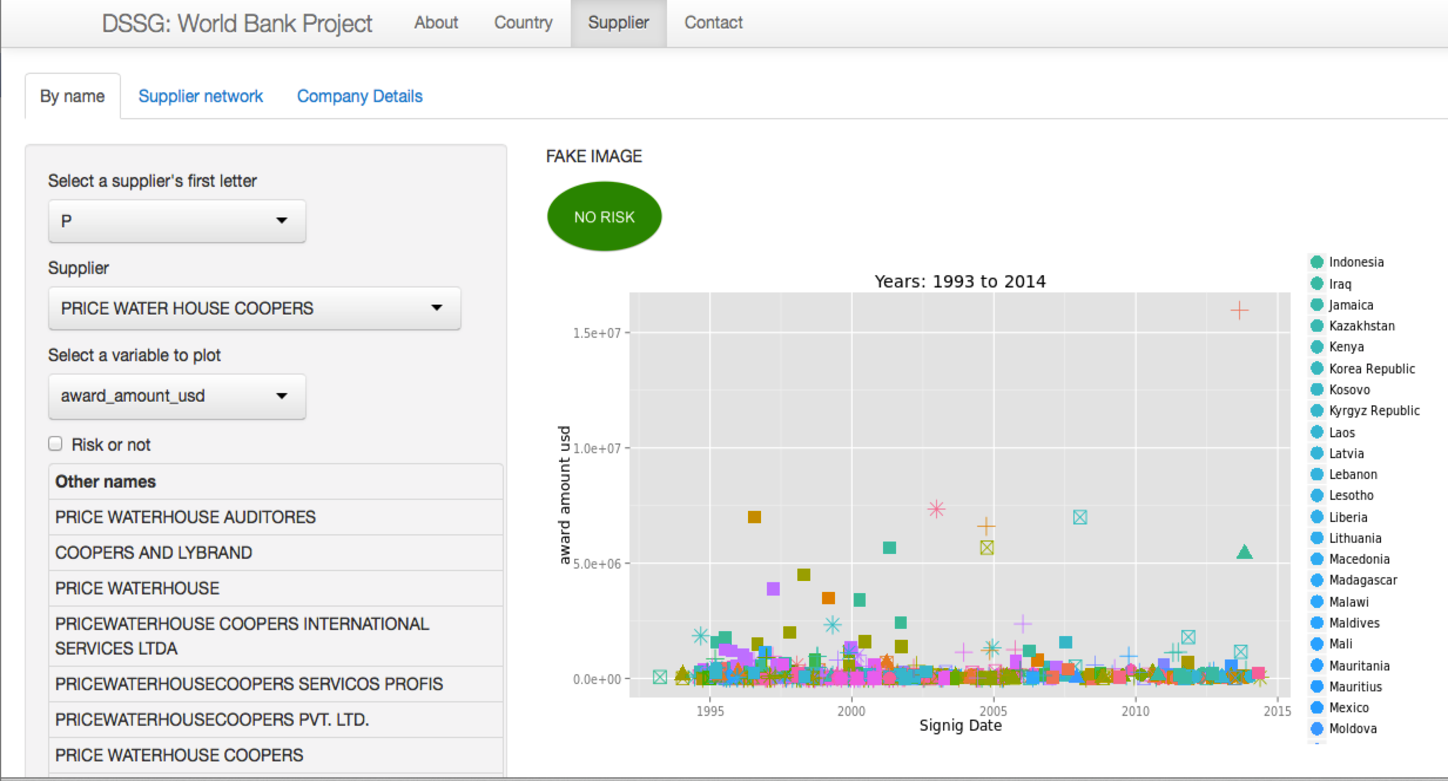
\includegraphics[width=1.05\textwidth,keepaspectratio]{../img/dashboard.pdf}
\end{center}
\noindent \footnotesize{\textbf{Source:} Own creation.}
\end{figure}


\subsection{Country tab: Red-flags from data}

After that, the \textit{Country tab} is designed to actually look for those red flags presented on the About tab but in real data form the historic and major awards as well as the investigations data. As chapter \ref{chap_procurements} presented figure \ref{fig_what_corr} suggesting ideas of how to look for common patterns to identify potential cases of corruption, collusion, fraud, coercion and other types of malicious behavior among the procurements that the World Bank gives to countries all over the world. The objective of this tab is to try to replicate those figures by using real data in order to provide a valuable insight to the investigators working in the Integrity Vice Presidency to help them attack this problem.

For example, this tab shows images such as \ref{fig_mex-top15} and \ref{fig_mex-amount}. To start, figure  \ref{fig_mex-top15}shows possible cases of collusion in Mexico. It shows the top 15 contracts in terms of awarded amount. This figure tries to replicate figure \ref{fig_cum_value} by showing that that only few contractors are getting almost all the contracts, as much as 30\% in Mexico and actually it's going only to few states.
% \begin{figure}[H]
% \begin{center}
% \caption{Red Flags: top 15 contracts in Mexico}
% \label{fig_mex-many}
% 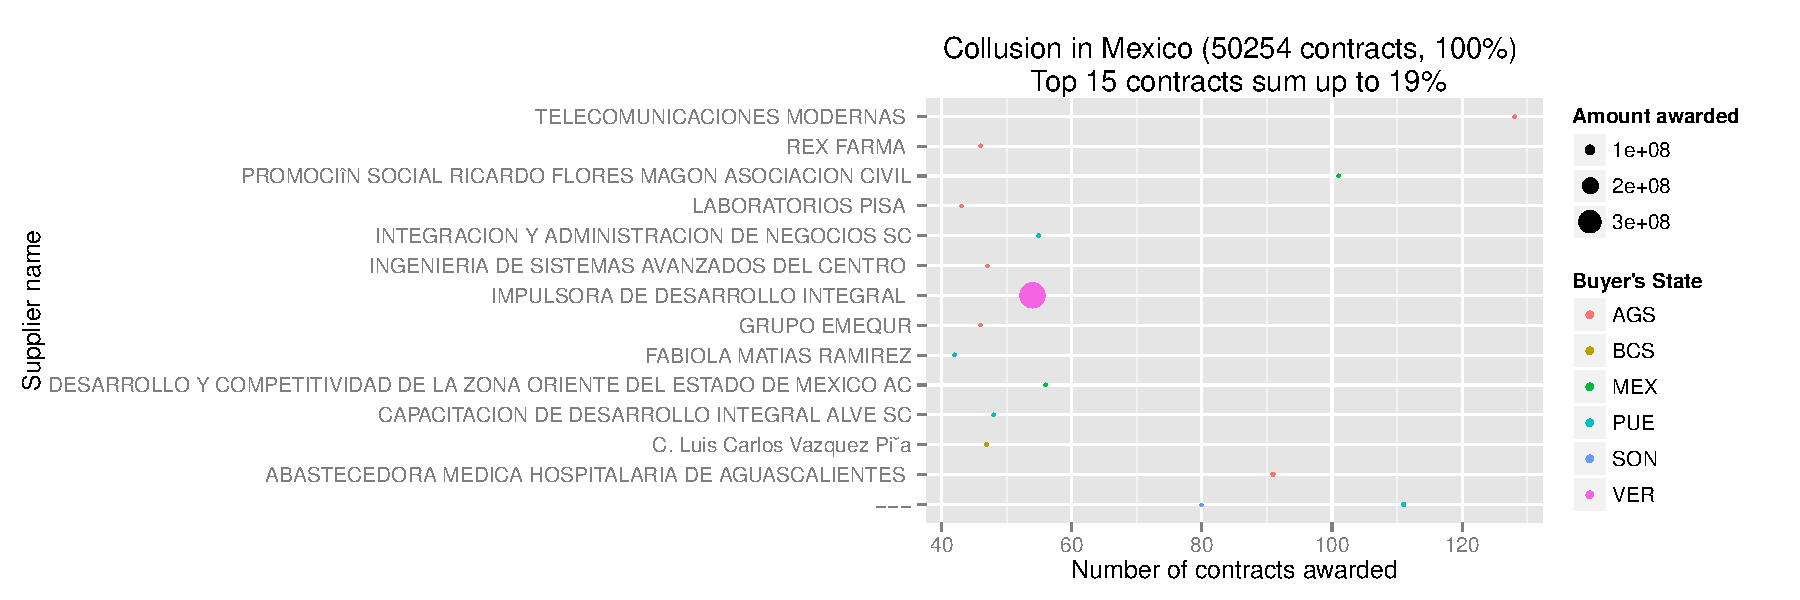
\includegraphics[width=1.05\textwidth,keepaspectratio]{../img/mex_many-15.pdf}
% \end{center}
% \noindent \footnotesize{\textbf{Source:} Own creation.}
% \end{figure}
\begin{figure}[H]
\begin{center}
\caption{Red Flags: top 15 contracts in Mexico}
\label{fig_mex-top15}
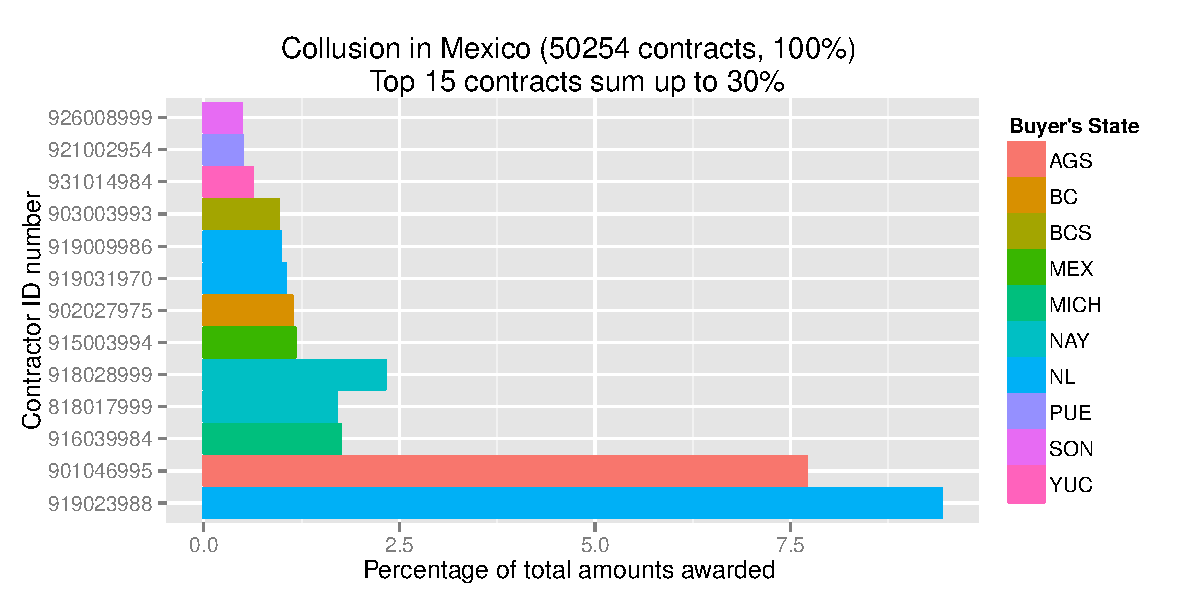
\includegraphics[width=1.05\textwidth,keepaspectratio]{../img/mex-top-15.pdf}
\end{center}
\noindent \footnotesize{\textbf{Source:} Own creation.}
\end{figure}


Then, figure \ref{fig_mex-amount} shows the distribution of number of contracts against the awarded amount per supplier and colored by the State. This figure helps them identify outliers in the procurements. It shows that, as expected, there are few contractors that are receiving contracts with very big awarded amounts in USD against suppliers that are receiving a considerable bigger amount of small contracts compared to the majority of the suppliers. This might or might not be indicators of corruption, collusion or fraud, but it helps the investigators to identify what suppliers are receiving more in terms of money or contracts such that they can keep closer attention.


\begin{figure}[H]
\begin{center}
\caption{Red Flags: Outliers in Mexico}
\label{fig_mex-amount}
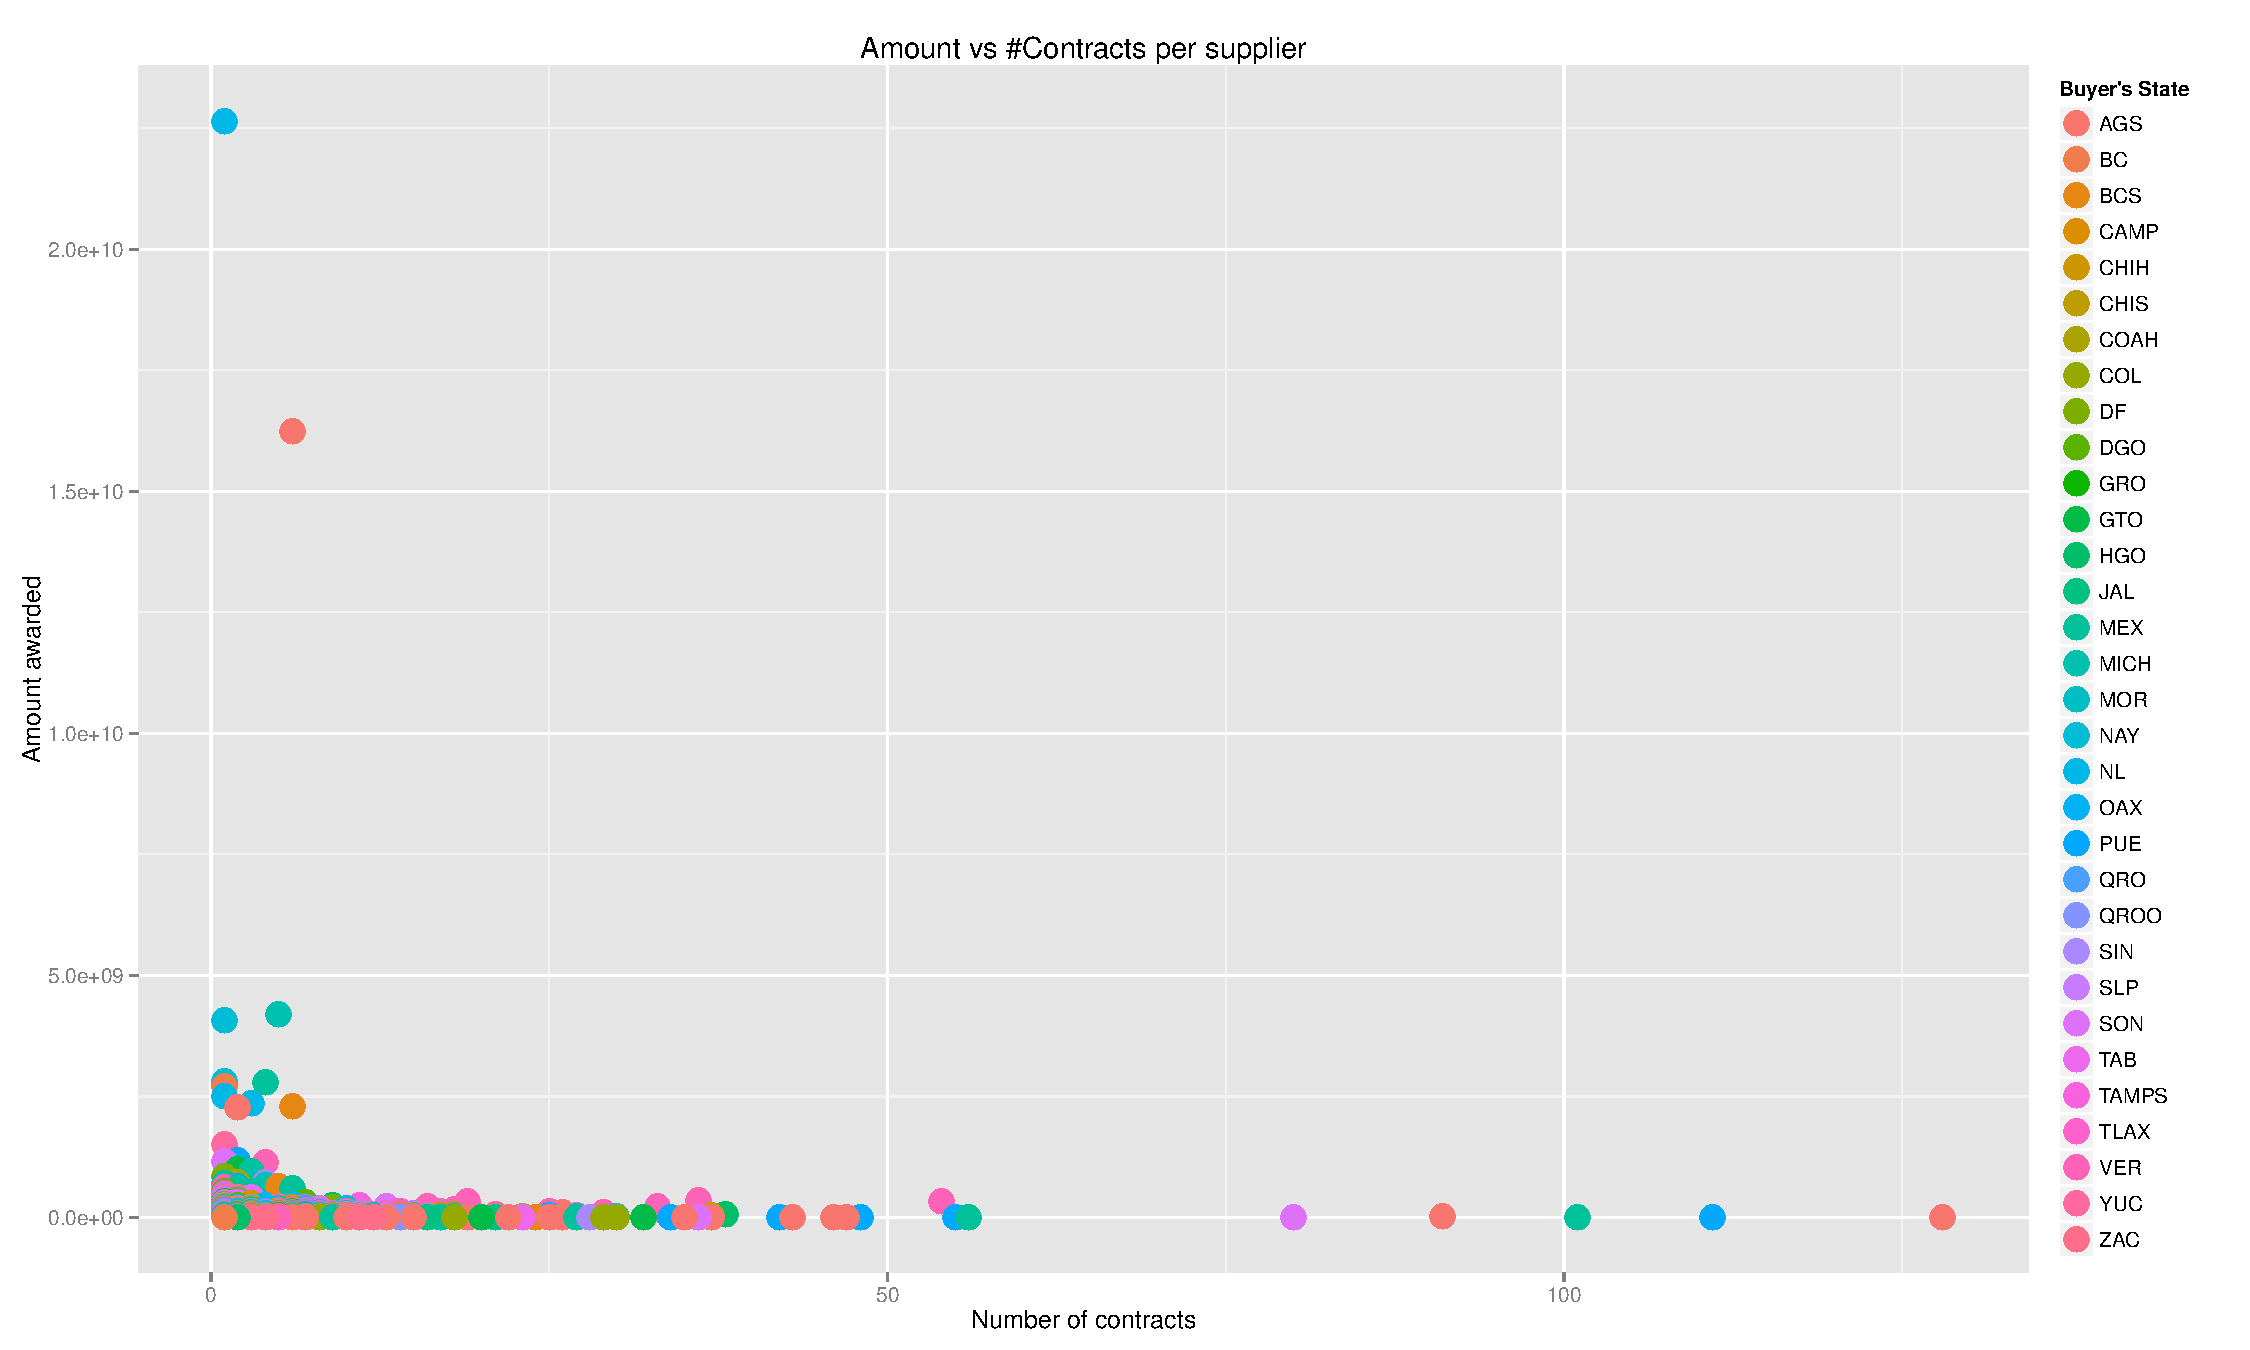
\includegraphics[width=1.05\textwidth,keepaspectratio]{../img/mex-amount-contract.pdf}
\end{center}
\noindent \footnotesize{\textbf{Source:} Own creation.}
\end{figure}

\subsection{Supplier tab: Name disambiguation, model \& network}

The next tab in the dashboard is the \textit{Supplier tab} which is the most relevant because it displays the result of the model and the one displayed at figure \ref{fig_dashboard}. In this tab the investigators at the World Bank can select a specific entity to look at. For example, figure \ref{fig_dashboard} shows the case of Price Waterhouse Coopers. The first thing to notice is that the dashboard displays a long list of names under the `Other names' subtitle. Those names show the results of the Google search algorithm, i.e. all the other names by which an investigator might find the entity Price Waterhouse Coppers among the different databases form the World Bank. The list can be downloaded for future reference. This tab also shows a plot to display any of the desired numeric variable against time  for that specific contractor and colored by country so that investigators can look for suspicious patterns.

Maybe the most important part of this tab and the dashboard is the \textit{Risk factor icon}. As it can be seen from figure \ref{fig_dashboard}, after the investigator has selected an entity, the dashboard displays an icon that represent the level of risk that entity has in the random forest. This is the most valuable item in the dashboard because it helps the investigator to confirm whether their suspiciousness for an entity is solid enough for them to take action into a deeper investigation. There are three categories for risk that include: no risk, low risk and high risk. The classification in those categories was very conservative so that it helps them to identify cases that require major attention. The figure \ref{fig_risk_map} is an static image that shows the risk factor among the World. It summarizes the results of the model and the risk item shown in the dashboard.

\subsubsection{Contract specific risk map}

\begin{figure}[H]
\begin{center}
\caption{Risk map (Sample)}
\label{fig_risk_map}
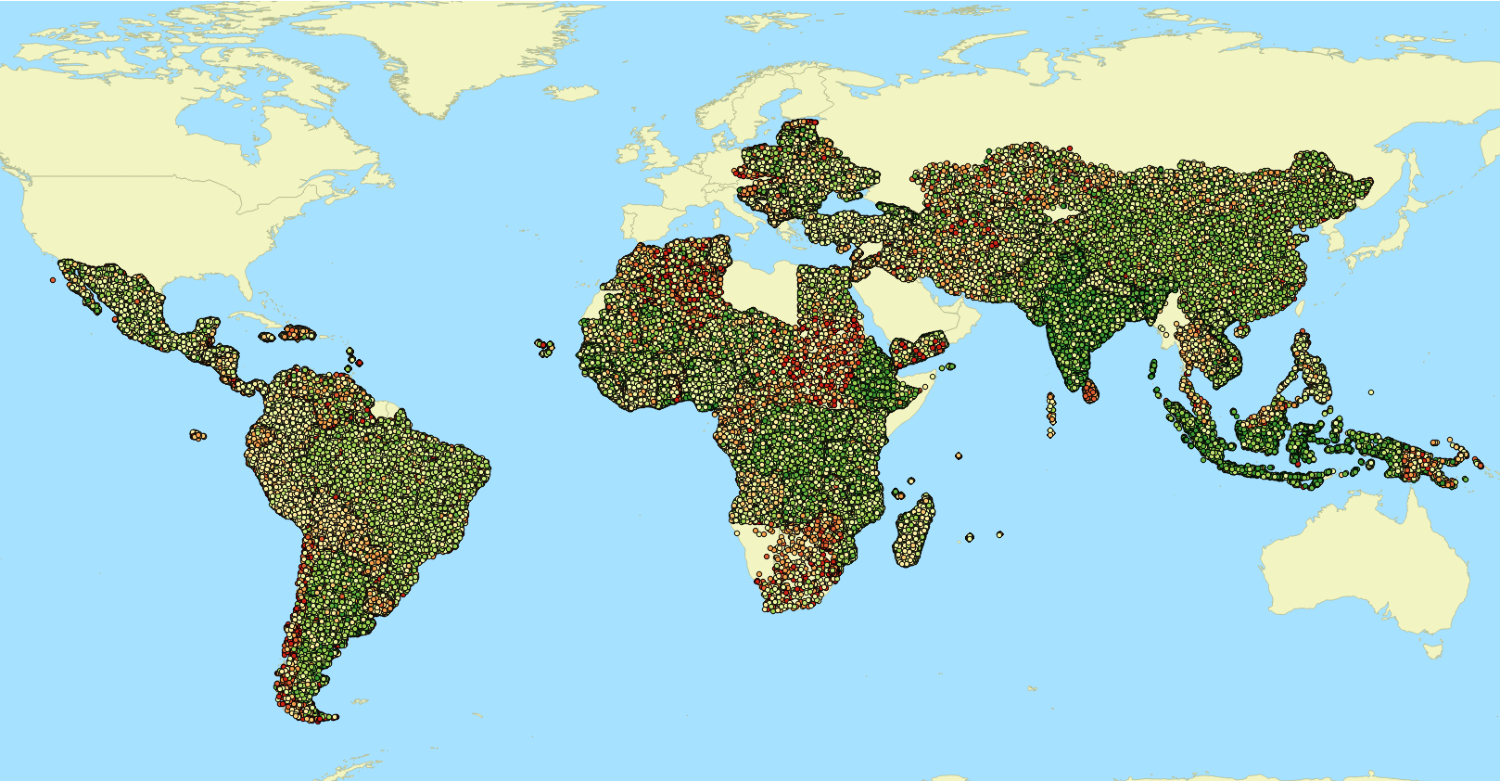
\includegraphics[width=\textwidth,height=1\textheight,keepaspectratio]{../img/risk_map.pdf}
\end{center}
\noindent \footnotesize{\textbf{Source:} Own creation based on \cite{wb_i_map}. \\Data from the World Bank \parencite{wb_data}.}
\end{figure}



After that, the sub tab \textit{Supplier network} shows the one degree co-award live network for the entity selected. Figure \ref{fig_network} is an example of what this tab shows. In this tab the user can also download the data from the network for future reference along with the data from the neighbors that where investigated.

Finally, sub tab \textit{Company details} shows all the data available to download referring to the entity selected in the previous tab so that the investigators can explore with detail each one of the projects where the entity participated. It includes data for the projects awarded and not awarded but where it participated as a bidder, which might help them to identify collusion or coercion.

\subsection{Interactive map}

Finally, there is a second visualization created for the investigators at the World Bank, an interactive map that shows the evolution of the contracts in time. This visualization was developed in collaboration with the participants of the Data sprint hackathon organized with the World Bank. There is a public version available at \href{http://detecting-corruption.carlospetricioli.com/interactive_map}{detecting-corruption.carlospetricioli.com/interactive\_map}. The map displays how contracts accumulate in time among the countries to which the World Bank gives contracts to. The color corresponds to the sector in the project. If you point to any of countries, the visualization displays the amount borrowed and supplied from/to that country. If you click on any of the flying dots, which refers to a specific country and flies from the supplier country to the borrowed one, it displays the data. It includes the name of the project, the product line, the major sector, the type of procurement, the method of selection, the category, the region as well as the amount. This visualization is just one more way for the investigators to study the behavior of the contracts among the world and can be used in hand with the risk map shown in figure \ref{fig_risk_map} to identify potential risk factors.


\begin{figure}[H]
\begin{center}
\caption{Interactive map}
\label{fig_interactive_map}
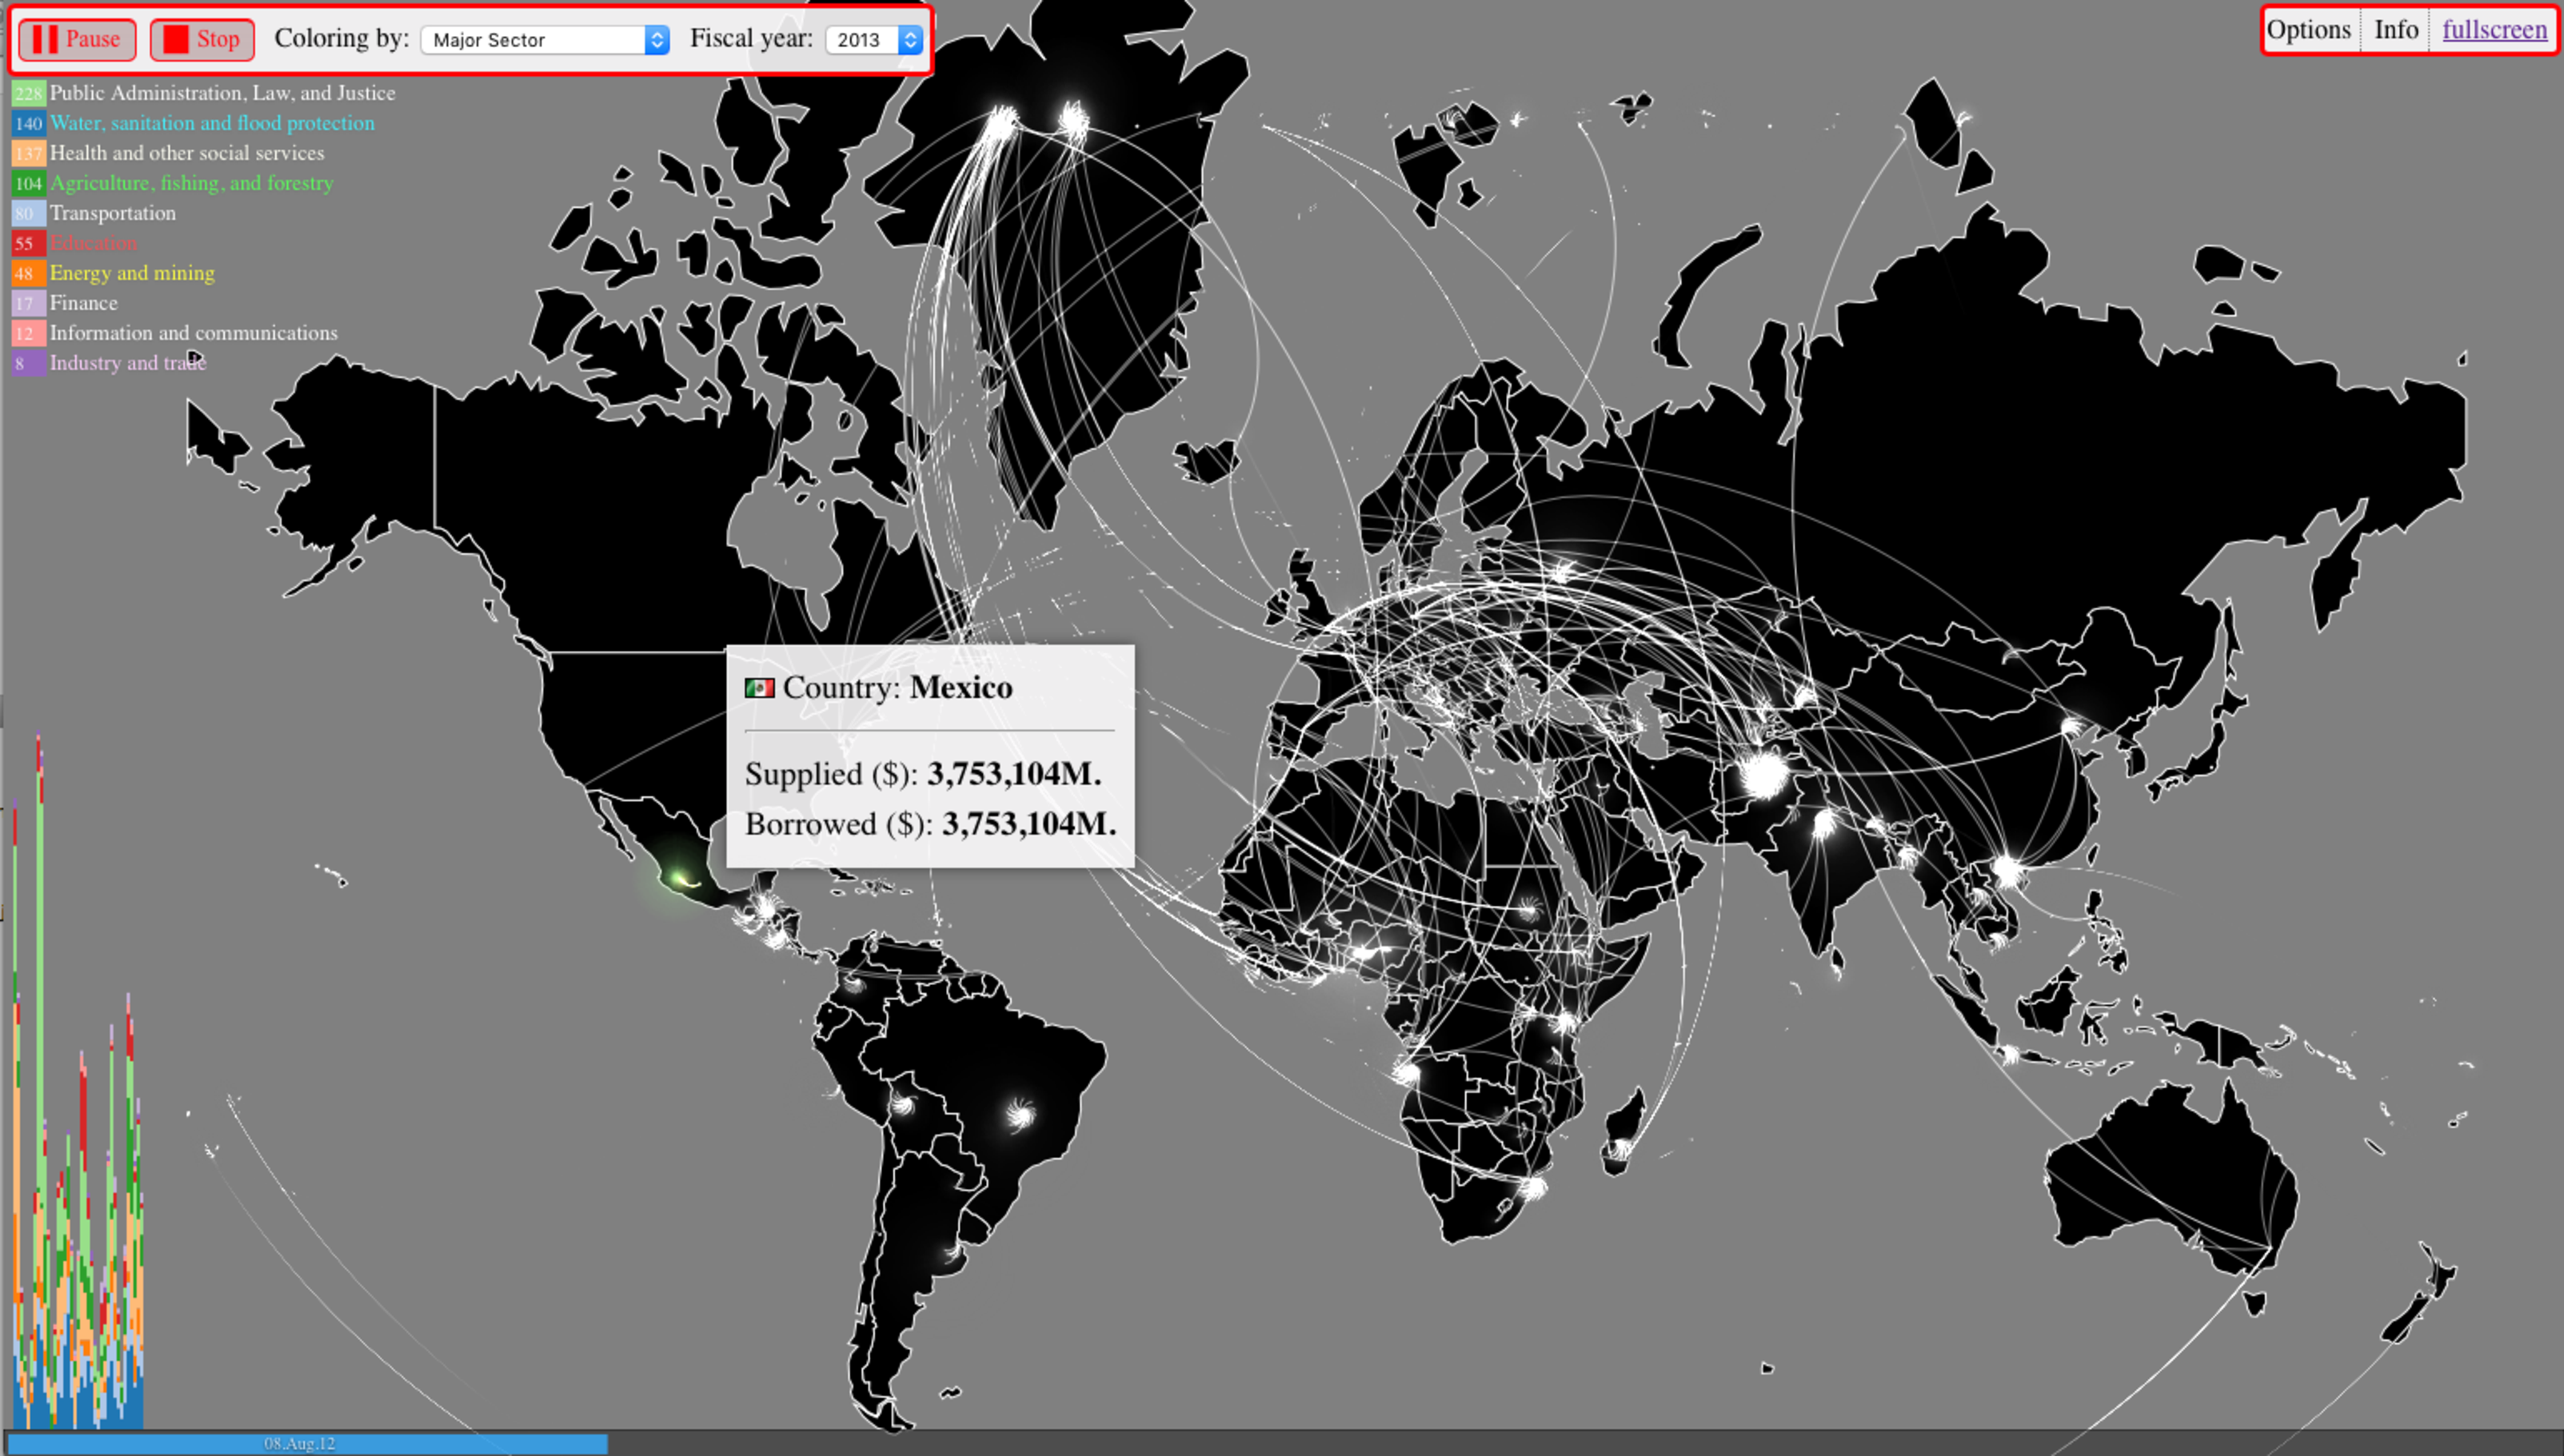
\includegraphics[width=\textwidth,height=1\textheight,keepaspectratio]{../img/interactive_map_mex.pdf}
\end{center}
\noindent \footnotesize{\textbf{Source:} Own creation based on \cite{wb_i_map}. \\Go to \href{http://detecting-corruption.carlospetricioli.com/interactive_map}{detecting-corruption.carlospetricioli.com/interactive\_map} to see a live version. \\Data from the World Bank \parencite{wb_data}.}
\end{figure}






\chapter{Conclusion}\label{chap_conclusion}

From this project it is clear that identifying potential cases of corruption, collusion  and fraud is a difficult task. The good part is that there is a lot of space for improvement in the investigation process that the Integrity Vice Presidency performs. By now, they rely on whistle-blowers and third parties to fill complicated forms in their web  and mobile applications or to place calls to the World Bank so that they are able to start an investigation process that could be just based on competitors that are trying to slow the procurement process. Fortunately for them this project represents a viable way for them to perform investigations in a proactive way instead of having to wait for third parties to give them actionable arguments to investigate an entity or a project. Not only that, they can make their decisions based on objective data that might also help to prioritize their investigations so that they target the ones that have more impact.

This project showed that current data collected by World Bank on contracts is sufficient to forecast risk on future contracts, and as explained, these risk forecasts can allow World Bank investigators to be more proactive in determining which companies, projects and contracts to examine. This project suggest that future data collection should be done in a more standardized way such that they do not need to rely on an algorithm such as the Google searches algorithm  so that they are able to identify entities among different data sources within their own data. This might lead to changes in the way they start the procurements process, but this work is a clear example of the impact that a small change in the way they collect data from entities all over the world can make a huge difference. After modifying the way they collect data, future analysis could be able to identify separate risk levels for fraud, collusion and corruption.

Finally, this project serves as an example of how a real life problem should be approached as a data science problem, it demonstrates the importance of the relation between the partner and the data scientists and illustrates all the necessary elements a project like this should have.


% C. 
\appendix

%%%%%%%%%%%%%%%%%%%%%%%%%%%%%%%%%%%%
\titleformat{\chapter} % command
[display] % shape
{\bfseries \LARGE} % format
{\rule{\textwidth}{0.9pt} Appendix \ \thechapter.} % label
{0.0ex} % sep
{   \centering } 
[
\vspace{-0.9ex}%
\rule{\textwidth}{0.3pt}
] % after-code
%%%%%%%%%%%%%%%%%%%%%%%%%%%%%%%%%%%%


% !TEX root = A0_thesis_detecting_collusion_corruption_fraud.tex
\chapter{Sample Procurement Plan}\label{app_proc_plan}

\noindent\textit{(Text  in italic font is meant for instruction to staff and should be deleted in the final version of the  PP)}

\textit{(This is only a sample with the minimum content that is required to be included in the PAD. The detailed procurement plan is still mandatory for disclosure on the Bank's website in accordance with the guidelines. The initial procurement plan will cover the first 18 months of the project and then updated annually or earlier as necessary).
}
\begin{enumerate}[I.]
\item 	General
	\begin{enumerate}[1.]
	\item \textbf{Bank's approval Date of the procurement Plan} \textcolor{blue}{\textit{[Original: December 2007]: Revision 15 of Updated Procurement Plan, June 2010]}}
	\item \textbf{Date of General Procurement Notice}: \textcolor{blue}{\textit{Dec 24, 2006}}
	\item \textbf{Period covered by this procurement plan}: \textcolor{blue}{\textit{The procurement period of project covered from year June 2010 to December 2012}}
	\end{enumerate}

\item Goods and Works and non-consulting services.

	\begin{enumerate}[1.]

	\item	\textbf{Prior Review Threshold}: Procurement Decisions subject to Prior Review by the Bank as stated in Appendix 1 to the Guidelines for Procurement: \textit{[Thresholds for applicable procurement methods (not limited to the list below) will be determined by the Procurement Specialist /Procurement Accredited Staff based on the assessment of the implementing agency's capacity.]}

	\begin{table}[H]
	\caption{Prior Review Threshold}
	\resizebox{\textwidth}{!}{
	\begin{tabular}{|l|l|r|r|}
	\hline
	& \textbf{Procurement Method}	& \textbf{Prior Review Threshold US\$} &\textbf{Comments} \\
	\hline
	1.	& ICB and LIB (Goods) &	\textcolor{blue}{\textit{Above US\$ 500,000}}	& \textcolor{blue}{\textit{All}} \\
	2.	& NCB (Goods) & \textcolor{blue}{\textit{Above US\$ 100,000}}		& \textcolor{blue}{\textit{First contract}} \\
	3.	& ICB (Works) & \textcolor{blue}{\textit{Above US\$ 15 million}} & \textcolor{blue}{\textit{All}} \\
	4.	& NCB (Works) & \textcolor{blue}{\textit{Above US\$ 5 million}}	& \textcolor{blue}{\textit{All}} \\ 
	5.	& (Non Consultant Services)	& \textcolor{blue}{\textit{Below US\$ 100,000}}	& \textcolor{blue}{\textit{First contract}} \\
	    & [Add other methods if necessary]	& & 	\\
	    \hline
	\end{tabular}
	}
	\footnotesize{\textbf{Source} \cite{wb_sample_proc}.}
	\end{table}

	\item	\textbf{Prequalification}. Bidders for \textcolor{blue}{\textit{\underline{Not Aplicable}}} shall be prequalified in accordance with the provisions of paragraphs 2.9 and 2.10 of the Guidelines.

	\item	\textbf{Proposed Procedures for CDD Components (as per paragraph. 3.17 of the Guidelines):} \textit{[Refer to the relevant CDD project implementation document approved by the Bank or delete if not applicable]}

	\item	\textbf{Reference to (if any) Project Operational/Procurement Manual:} \textcolor{blue}{\textit{Project Implementation Manual for World Bank Loan Project XYZ  04/01/2010 issued by $<$ mention name of PIU$>$}}

	\item	\textbf{Any Other Special Procurement Arrangements:} \textit{[including advance procurement and retroactive financing, if applicable]} \textcolor{blue}{\textit{5 ICB works packages will be financed under retroactive financing}}

	\item	\textbf{Summary of the Procurement Packages planned during the first 18 months after project effectiveness \textit{( including those that are subject to retroactive financing and advanced procurement)}}

	\end{enumerate}
\textit{[List the Packages which require Bank's prior review first and then the other packages]}

	\begin{table}[H]
		\caption{Summary of the procurements packages}
		\resizebox{\textwidth}{!}{
		\begin{tabular}{|l|l|r|r|r|r|r|}
			\hline
		\textbf{Ref.}	& \multirow{2}{*}{ \textbf{Description}} & \textbf{Estimated Cost}  & \multirow{2}{*}{\textbf{Packages}} & \textbf{Domestic Preference}  &\textbf{Review by Bank} & \multirow{2}{*}{\textbf{Comments}}\\

		\textbf{No.}	&  &\textbf{US\$ million}  & &\textbf{(yes/no)}  &\textbf{(Prior/Post)} & \\
		

			\hline

		&Summary of the ICB	&	\multirow{2}{*}{ \textcolor{blue}{82}}	&	\multirow{2}{*}{ \textcolor{blue}{5}}	& \multirow{2}{*}{ \textcolor{blue}{No}}	& \multirow{2}{*}{ \textcolor{blue}{Prior}}	&  \\
		& (Works)	&		&		& 	& 	&  \\

		&Summary of the ICB	&	\multirow{2}{*}{ \textcolor{blue}{43.77}}	&	\multirow{2}{*}{ \textcolor{blue}{15}}	& \multirow{2}{*}{ \textcolor{blue}{No}}	& \multirow{2}{*}{ \textcolor{blue}{Prior}}	&  \\
		& (Goods)	&		&		& 	& 	&  \\

		&Summary of the ICB	&	\multirow{2}{*}{ \textcolor{blue}{64.53}}	&	\multirow{2}{*}{ \textcolor{blue}{18}}	& \multirow{2}{*}{ \textcolor{blue}{No}}	& \multirow{2}{*}{ \textcolor{blue}{Post}}	&  \textcolor{blue}{1st contact} \\
		& (Works)	&		&		& 	& 	&  \textcolor{blue}{for Prior Review}\\

		&Summary of the ICB	&	\multirow{2}{*}{ \textcolor{blue}{1.86}}	&	\multirow{2}{*}{ \textcolor{blue}{4}}	& \multirow{2}{*}{ \textcolor{blue}{No}}	& \multirow{2}{*}{ \textcolor{blue}{Post}}	&  \textcolor{blue}{1st contact} \\
		& (Goods)	&		&		& 	& 	&  \textcolor{blue}{for Prior Review}\\

		&Summary of the ICB	&	\multirow{2}{*}{ \textcolor{blue}{0.45}}	&	\multirow{2}{*}{ \textcolor{blue}{1}}	& \multirow{2}{*}{ \textcolor{blue}{No}}	& \multirow{2}{*}{ \textcolor{blue}{Prior}}	&  \\
		& (Non-Consultant Services)	&		&		& 	& 	&  \\
		    \hline
		\end{tabular}
		}
		\footnotesize{\textbf{Source} \cite{wb_sample_proc}.}
	\end{table}

\item Selection of Consultants

\begin{enumerate}[1.]
	\item \textbf{Prior Review Threshold}: Selection decisions subject to Prior Review by Bank as stated in Appendix 1 to the Guidelines Selection and Employment of Consultants:
	\begin{table}[H]
		\caption{Selection Method}
	\begin{center}
		\begin{tabular}{|l|l|r|r|}
				\hline
				\textbf{Ref.}	&  \textbf{Selection}  &  \textbf{Prior Review} & \multirow{2}{*}{\textbf{Comments}} \\
				\textbf{No.}	& Method & \textbf{Threshold}  &  \\
				\hline
	
				\multirow{2}{*}{1.}	& Competitive Methods   &  \textcolor{blue}{Above} &  \\
							& (Firms) & \textcolor{blue}{US\$ 100,000}  &  \\
	
				\multirow{2}{*}{2.}	& Single Source   	&  \multirow{2}{*}{\textcolor{blue}{All}} &  \\
									& (Firms)		&   &  \\
	
				\multirow{2}{*}{3.}	& \multirow{2}{*}{\textcolor{blue}{Individual}}   	&  \textcolor{blue}{Above} &  \\
									& 	   & \textcolor{blue}{US\$ 100,000}  &  \\
				\hline
			\end{tabular}
	\end{center}

	\footnotesize{\textbf{Source} \cite{wb_sample_proc}.}
	\end{table}

	\item \textbf{Short list comprising entirely of national consultants}: Short list of consultants for services, estimated to cost less than \textcolor{blue}{\underline{\$300,000}} equivalent per contract, may comprise entirely of national consultants in accordance with the provisions of paragraph 2.7 of the Consultant Guidelines.

	\item 	\textbf{Any Other Special Selection Arrangements}: \textit{[including advance procurement and retroactive financing, if applicable or delete if not applicable]}

	\item \textbf{Consultancy Assignments with Selection Methods and Time Schedule}

\begin{table}[H]
		\caption{Consultancy Assignments with Selection Methods and Time Schedule}
		\resizebox{\textwidth}{!}{
		\begin{tabular}{|l|l|r|r|r|r|}
			\hline
		\textbf{Ref.}	& \textbf{Description} & \textbf{Estimated Cost}  & \multirow{2}{*}{\textbf{Packages}}   &\textbf{Review by Bank} & \multirow{2}{*}{\textbf{Comments}} \\

		\textbf{No.} & \textbf{of Assignment}  &\textbf{US\$ million}  &   &\textbf{(Prior/Post)} &  \\
		

			\hline

		\multirow{3}{*}{1.}&Summary of the number &	\multirow{3}{*}{ \textcolor{blue}{4.17}}	&	\multirow{3}{*}{ \textcolor{blue}{7}}	& \multirow{3}{*}{ \textcolor{blue}{Prior}}	&   \\
		& of contracts that will&		& 	&  &	  \\
		&be lead under QCBC 	&		& & 	& 	  \\

		\multirow{3}{*}{2.}&Summary of the number &	\multirow{3}{*}{ \textcolor{blue}{0.83}}	&	\multirow{3}{*}{ \textcolor{blue}{1}}	& \multirow{3}{*}{ \textcolor{blue}{Prior}}	&  \multirow{3}{*}{ \textcolor{blue}{CQS}} \\
		& of contracts that will&		& 	&  &	  \\
		&be lead under other methods 	&		& & 	& 	  \\
		    \hline
		\end{tabular}
		}
		\footnotesize{\textbf{Source} \cite{wb_sample_proc}.}
	\end{table}



\end{enumerate}


\end{enumerate}







\chapter{Software}
\label{chap_software}

\noindent The software in used in this project is all free software. All the code was written using the  language \texttt{R Project for Statistical Computing}\footnote{``R is available as Free Software under the terms of the Free Software Foundation’s GNU General Public License in source code form. It compiles and runs on a wide variety of UNIX platforms and similar systems (including FreeBSD and Linux), Windows and MacOS.'' See \cite{r_pagina}.
} \footnote{See \cite{R:Bloomfield:2014} for an R user guide.}, and \textit{Python}\footnote{``Python is developed under an OSI-approved open source license, making it freely usable and distributable, even for commercial use. Python's license is administered by the Python Software Foundation.'' See \cite{python_about}.}. To summarize and visualize the data, all the graphs were made with \texttt{ggplot2} \parencite{wickham_ggplot} a package for R writen by Hadley Wickham. To create the global map using the spatial data, the project uses \texttt{Quantum-Gis (QGIS)}\footnote{See \cite{clifford1981} for details of what's spatial data.} \footnote{GIS refers to Geographical Information Systems and it refers to the set of techniques that uses spatial data, see \cite{GIS05}  for more details.}. To make the searches at Google using many Amazon Web Service's computers it uses \texttt{Parallel} \parencite{Tange2011a} to distribute the tasks. For the development, edition an writing, this project uses \LaTeX - A document preparation system \cite{latex}.
\chapter{World Bank countries}\label{chap_countries}


\begin{multicols}{3}
\scriptsize{
\noindent \texttt{ABW}	Aruba\\
\texttt{AFG}	Afghanistan\\
\texttt{AFR}	Africa\\
\texttt{AGO}	Angola\\
\texttt{ALB}	Albania\\
\texttt{AND}	Andorra\\
\texttt{ANR}	Andean Region\\
\texttt{ARB}	Arab World\\
\texttt{ARE}	United Arab Emirates\\
\texttt{ARG}	Argentina\\
\texttt{ARM}	Armenia\\
\texttt{ASM}	American Samoa\\
\texttt{ATG}	Antigua and Barbuda\\
\texttt{AUS}	Australia\\
\texttt{AUT}	Austria\\
\texttt{AZE}	Azerbaijan\\
\texttt{BDI}	Burundi\\
\texttt{BEL}	Belgium\\
\texttt{BEN}	Benin\\
\texttt{BFA}	Burkina Faso\\
\texttt{BGD}	Bangladesh\\
\texttt{BGR}	Bulgaria\\
\texttt{BHR}	Bahrain\\
\texttt{BHS}	Bahamas, The\\
\texttt{BIH}	Bosnia and Herzegovina\\
\texttt{BLR}	Belarus\\
\texttt{BLZ}	Belize\\
\texttt{BMU}	Bermuda\\
\texttt{BOL}	Bolivia\\
\texttt{BRA}	Brazil\\
\texttt{BRB}	Barbados\\
\texttt{BRN}	Brunei Darussalam\\
\texttt{BTN}	Bhutan\\
\texttt{BWA}	Botswana\\
\texttt{CAA}	Sub-Saharan Africa\\
(IFC classification)\\
\texttt{CAF}	Central African Republic\\
\texttt{CAN}	Canada\\
\texttt{CEA}	East Asia and the Pacific\\
(IFC classification)\\
\texttt{CEB}	Central Europe and the Baltics\\
\texttt{CEU}	Europe and Central Asia\\
(IFC classification)\\
\texttt{CHE}	Switzerland\\
\texttt{CHI}	Channel Islands\\
\texttt{CHL}	Chile\\
\texttt{CHN}	China\\
\texttt{CIV}	Cote d'Ivoire\\
\texttt{CLA}	Latin America and the Caribbean\\
(IFC classification)\\
\texttt{CME}	Middle East and North Africa\\
(IFC classification)\\
\texttt{CMR}	Cameroon\\
\texttt{COD}	Congo, Dem. Rep.\\
\texttt{COG}	Congo, Rep.\\
\texttt{COL}	Colombia\\
\texttt{COM}	Comoros\\
\texttt{CPV}	Cabo Verde\\
\texttt{CRI}	Costa Rica\\
\texttt{CSA}	South Asia\\
(IFC classification)\\
\texttt{CSS}	Caribbean small states\\
\texttt{CUB}	Cuba\\
\texttt{CUW}	Curacao\\
\texttt{CYM}	Cayman Islands\\
\texttt{CYP}	Cyprus\\
\texttt{CZE}	Czech Republic\\
\texttt{DEU}	Germany\\
\texttt{DJI}	Djibouti\\
\texttt{DMA}	Dominica\\
\texttt{DNK}	Denmark\\
\texttt{DOM}	Dominican Republic\\
\texttt{DZA}	Algeria\\
\texttt{EAP}	East Asia \& Pacific\\
(developing only)\\
\texttt{EAS}	East Asia \& Pacific\\
(all income levels)\\
\texttt{ECA}	Europe \& Central Asia\\
(developing only)\\
\texttt{ECS}	Europe \& Central Asia\\
(all income levels)\\
\texttt{ECU}	Ecuador\\
\texttt{EGY}	Egypt, Arab Rep.\\
\texttt{EMU}	Euro area\\
\texttt{ERI}	Eritrea\\
\texttt{ESP}	Spain\\
\texttt{EST}	Estonia\\
\texttt{ETH}	Ethiopia\\
\texttt{EUU}	European Union\\
\texttt{FCS}	Fragile and conflict affected situations\\
\texttt{FIN}	Finland\\
\texttt{FJI}	Fiji\\
\texttt{FRA}	France\\
\texttt{FRO}	Faeroe Islands\\
\texttt{FSM}	Micronesia, Fed. Sts.\\
\texttt{GAB}	Gabon\\
\texttt{GBR}	United Kingdom\\
\texttt{GEO}	Georgia\\
\texttt{GHA}	Ghana\\
\texttt{GIN}	Guinea\\
\texttt{GMB}	Gambia, The\\
\texttt{GNB}	Guinea-Bissau\\
\texttt{GNQ}	Equatorial Guinea\\
\texttt{GRC}	Greece\\
\texttt{GRD}	Grenada\\
\texttt{GRL}	Greenland\\
\texttt{GTM}	Guatemala\\
\texttt{GUM}	Guam\\
\texttt{GUY}	Guyana\\
\texttt{HIC}	High income\\
\texttt{HKG}	Hong Kong SAR, China\\
\texttt{HND}	Honduras\\
\texttt{HPC}	Heavily indebted poor countries\\
(HIPC)\\
\texttt{HRV}	Croatia\\
\texttt{HTI}	Haiti\\
\texttt{HUN}	Hungary\\
\texttt{IDN}	Indonesia\\
\texttt{IMN}	Isle of Man\\
\texttt{IND}	India\\
\texttt{INX}	Not classified\\
\texttt{IRL}	Ireland\\
\texttt{IRN}	Iran, Islamic Rep.\\
\texttt{IRQ}	Iraq\\
\texttt{ISL}	Iceland\\
\texttt{ISR}	Israel\\
\texttt{ITA}	Italy\\
\texttt{JAM}	Jamaica\\
\texttt{JOR}	Jordan\\
\texttt{JPN}	Japan\\
\texttt{KAZ}	Kazakhstan\\
\texttt{KEN}	Kenya\\
\texttt{KGZ}	Kyrgyz Republic\\
\texttt{KHM}	Cambodia\\
\texttt{KIR}	Kiribati\\
\texttt{KNA}	St. Kitts and Nevis\\
\texttt{KOR}	Korea, Rep.\\
\texttt{KSV}	Kosovo\\
\texttt{KWT}	Kuwait\\
\texttt{LAC}	Latin America \& Caribbean\\
(developing only)\\
\texttt{LAO}	Lao PDR\\
\texttt{LBN}	Lebanon\\
\texttt{LBR}	Liberia\\
\texttt{LBY}	Libya\\
\texttt{LCA}	St. Lucia\\
\texttt{LCN}	Latin America \& Caribbean\\
(all income levels)\\
\texttt{LCR}	Latin America and the Caribbean\\
\texttt{LDC}	Least developed countries: \\
UN classification\\
\texttt{LIC}	Low income\\
\texttt{LIE}	Liechtenstein\\
\texttt{LKA}	Sri Lanka\\
\texttt{LMC}	Lower middle income\\
\texttt{LMY}	Low \& middle income\\
\texttt{LSO}	Lesotho\\
\texttt{LTU}	Lithuania\\
\texttt{LUX}	Luxembourg\\
\texttt{LVA}	Latvia\\
\texttt{MAC}	Macao SAR, China\\
\texttt{MAF}	St. Martin\\
(French part)\\
\texttt{MAR}	Morocco\\
\texttt{MCA}	Central America\\
\texttt{MCO}	Monaco\\
\texttt{MDA}	Moldova\\
\texttt{MDE}	Middle East\\
(developing only)\\
\texttt{MDG}	Madagascar\\
\texttt{MDV}	Maldives\\
\texttt{MEA}	Middle East \& North Africa\\
(all income levels)\\
\texttt{MEX}	Mexico\\
\texttt{MHL}	Marshall Islands\\
\texttt{MIC}	Middle income\\
\texttt{MKD}	Macedonia, FYR\\
\texttt{MLI}	Mali\\
\texttt{MLT}	Malta\\
\texttt{MMR}	Myanmar\\
\texttt{MNA}	Middle East \& North Africa\\
(developing only)\\
\texttt{MNE}	Montenegro\\
\texttt{MNG}	Mongolia\\
\texttt{MNP}	Northern Mariana Islands\\
\texttt{MOZ}	Mozambique\\
\texttt{MRT}	Mauritania\\
\texttt{MUS}	Mauritius\\
\texttt{MWI}	Malawi\\
\texttt{MYS}	Malaysia\\
\texttt{NAC}	North America\\
\texttt{NAF}	North Africa\\
\texttt{NAM}	Namibia\\
\texttt{NCL}	New Caledonia\\
\texttt{NER}	Niger\\
\texttt{NGA}	Nigeria\\
\texttt{NIC}	Nicaragua\\
\texttt{NLD}	Netherlands\\
\texttt{NOC}	High income: nonOECD\\
\texttt{NOR}	Norway\\
\texttt{NPL}	Nepal\\
\texttt{NZL}	New Zealand\\
\texttt{OEC}	High income: OECD\\
\texttt{OED}	OECD members\\
\texttt{OMN}	Oman\\
\texttt{OSS}	Other small states\\
\texttt{PAK}	Pakistan\\
\texttt{PAN}	Panama\\
\texttt{PER}	Peru\\
\texttt{PHL}	Philippines\\
\texttt{PLW}	Palau\\
\texttt{PNG}	Papua New Guinea\\
\texttt{POL}	Poland\\
\texttt{PRI}	Puerto Rico\\
\texttt{PRK}	Korea, Dem. Rep.\\
\texttt{PRT}	Portugal\\
\texttt{PRY}	Paraguay\\
\texttt{PSE}	West Bank and Gaza\\
\texttt{PSS}	Pacific island small states\\
\texttt{PYF}	French Polynesia\\
\texttt{QAT}	Qatar\\
\texttt{ROU}	Romania\\
\texttt{RUS}	Russian Federation\\
\texttt{RWA}	Rwanda\\
\texttt{SAS}	South Asia\\
\texttt{SAU}	Saudi Arabia\\
\texttt{SCE}	Southern Cone\\
\texttt{SDN}	Sudan\\
\texttt{SEN}	Senegal\\
\texttt{SGP}	Singapore\\
\texttt{SLB}	Solomon Islands\\
\texttt{SLE}	Sierra Leone\\
\texttt{SLV}	El Salvador\\
\texttt{SMR}	San Marino\\
\texttt{SOM}	Somalia\\
\texttt{SRB}	Serbia\\
\texttt{SSA}	Sub-Saharan Africa\\
(developing only)\\
\texttt{SSD}	South Sudan\\
\texttt{SSF}	Sub-Saharan Africa\\
(all income levels)\\
\texttt{SST}	Small states\\
\texttt{STP}	Sao Tome and Principe\\
\texttt{SUR}	Suriname\\
\texttt{SVK}	Slovak Republic\\
\texttt{SVN}	Slovenia\\
\texttt{SWE}	Sweden\\
\texttt{SWZ}	Swaziland\\
\texttt{SXM}	Sint Maarten\\
(Dutch part)\\
\texttt{SXZ}	Sub-Saharan Africa \\
excluding South Africa\\
\texttt{SYC}	Seychelles\\
\texttt{SYR}	Syrian Arab Republic\\
\texttt{TCA}	Turks and Caicos Islands\\
\texttt{TCD}	Chad\\
\texttt{TGO}	Togo\\
\texttt{THA}	Thailand\\
\texttt{TJK}	Tajikistan\\
\texttt{TKM}	Turkmenistan\\
\texttt{TLS}	Timor-Leste\\
\texttt{TON}	Tonga\\
\texttt{TTO}	Trinidad and Tobago\\
\texttt{TUN}	Tunisia\\
\texttt{TUR}	Turkey\\
\texttt{TUV}	Tuvalu\\
\texttt{TWN}	Taiwan, China\\
\texttt{TZA}	Tanzania\\
\texttt{UGA}	Uganda\\
\texttt{UKR}	Ukraine\\
\texttt{UMC}	Upper middle income\\
\texttt{URY}	Uruguay\\
\texttt{USA}	United States\\
\texttt{UZB}	Uzbekistan\\
\texttt{VCT}	St. Vincent and the Grenadines\\
\texttt{VEN}	Venezuela, RB\\
\texttt{VIR}	Virgin Islands (U.S.)\\
\texttt{VNM}	Vietnam\\
\texttt{VUT}	Vanuatu\\
\texttt{WLD}	World\\
\texttt{WSM}	Samoa\\
\texttt{XZN}	Sub-Saharan Africa \\
excluding South Africa and Nigeria\\
\texttt{YEM}	Yemen, Rep.\\
\texttt{ZAF}	South Africa\\
\texttt{ZMB}	Zambia\\
\texttt{ZWE}	Zimbabwe
}
\end{multicols}




\section{World Bank's World Development Indicators} \label{sec_wdi}
\begin{figure}[H]
\begin{center}
\caption{WDI: Transparency Accountability Corruption Rating, Country/Region}
\label{fig_wdi_transp}
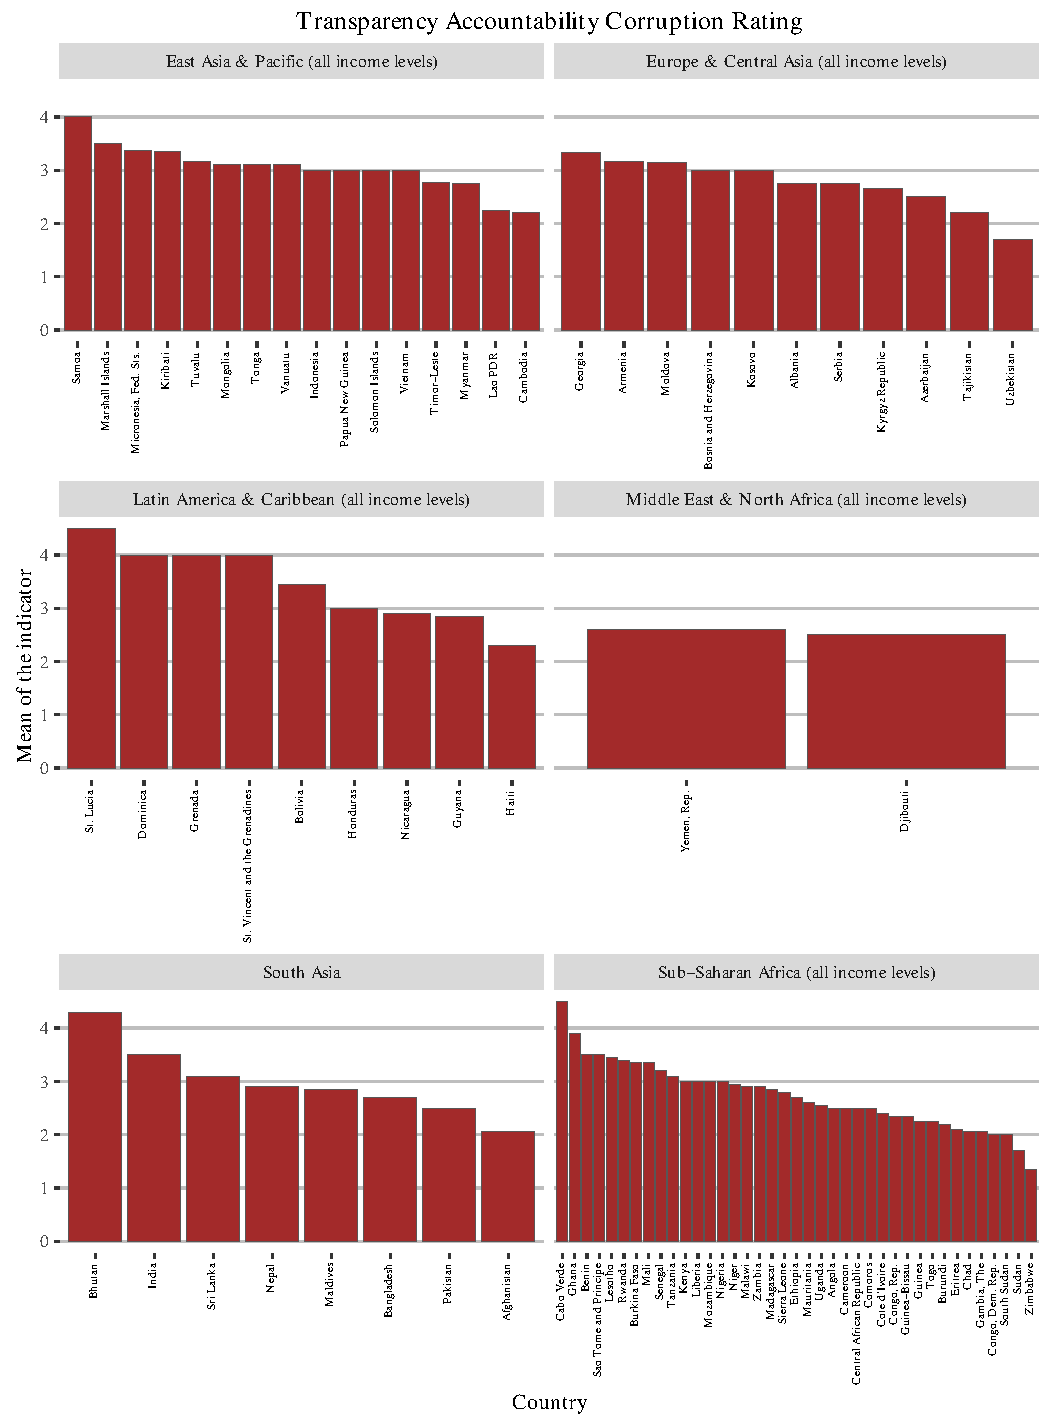
\includegraphics[max height=.82\textheight]{../img/wdi_transparency_accountability_corruption_rating.pdf}
\end{center}
\noindent \footnotesize{\textbf{Source:} Own creation and data obtained with package \texttt{WDI}, see the \cite{wb_r}.}
\end{figure}

\begin{figure}[H]
\begin{center}
\caption{WDI: Property Rights Rule Governance Rating per Country/Region}
\label{fig_wdi_prop}
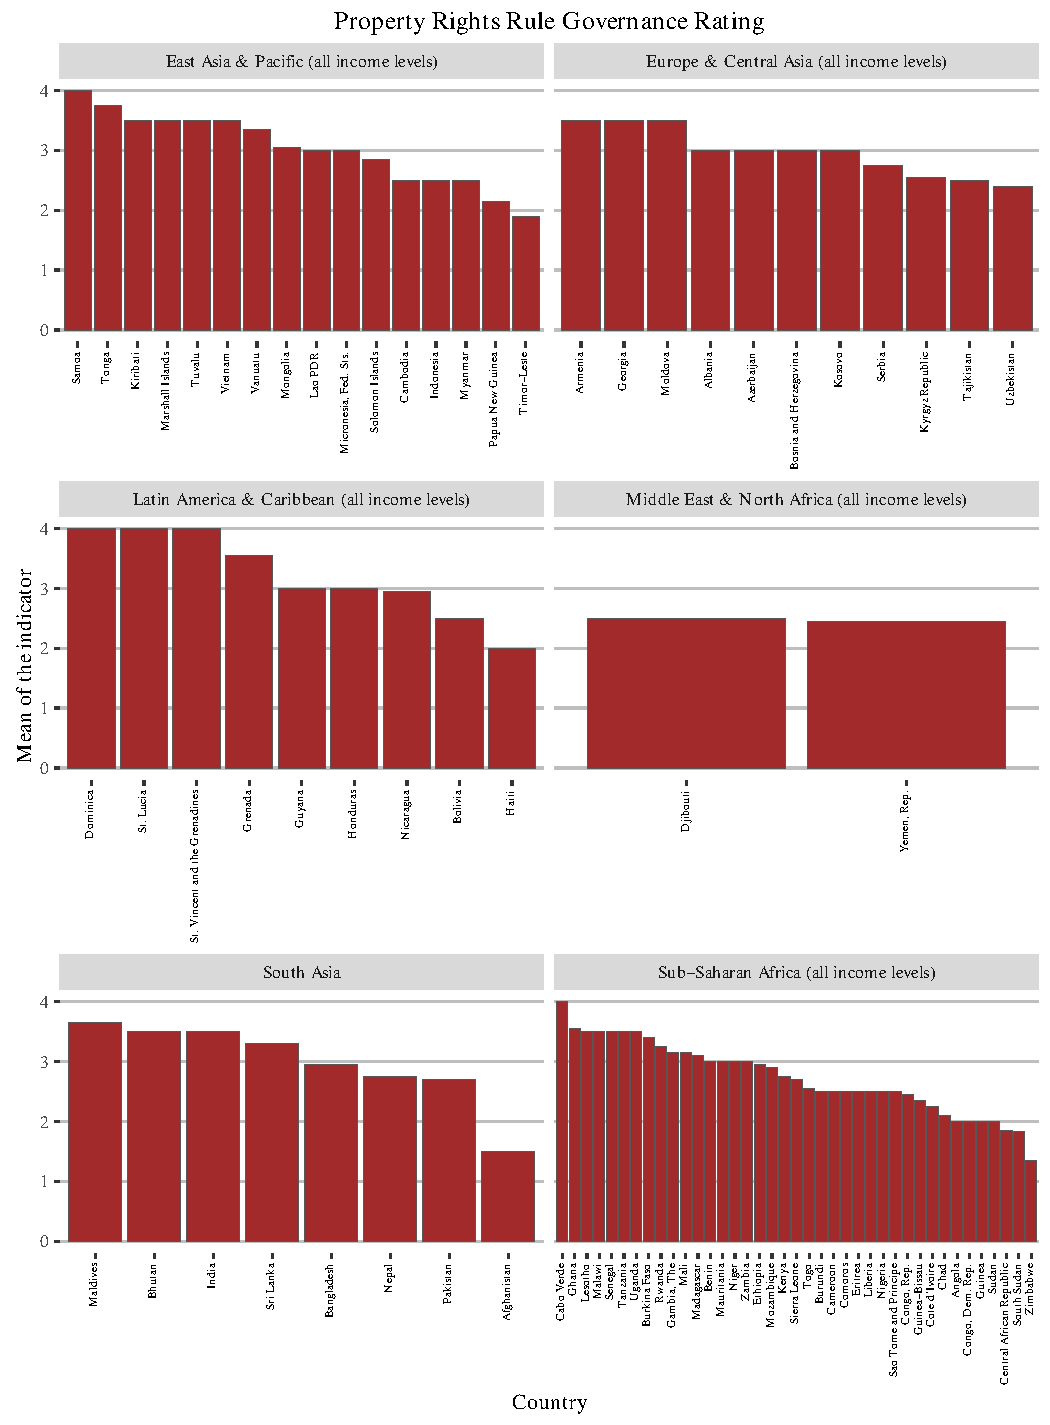
\includegraphics[height=.9\textheight]{../img/wdi_property_rights_rule_governance_rating.pdf}
\end{center}
\noindent \footnotesize{\textbf{Source:} Own creation and data obtained with package \texttt{WDI}, see the \cite{wb_r}.}
\end{figure}

\begin{figure}[H]
\begin{center}
\caption{WDI: Legal Rights Index per Country/Region}
\label{fig_wdi_legal}
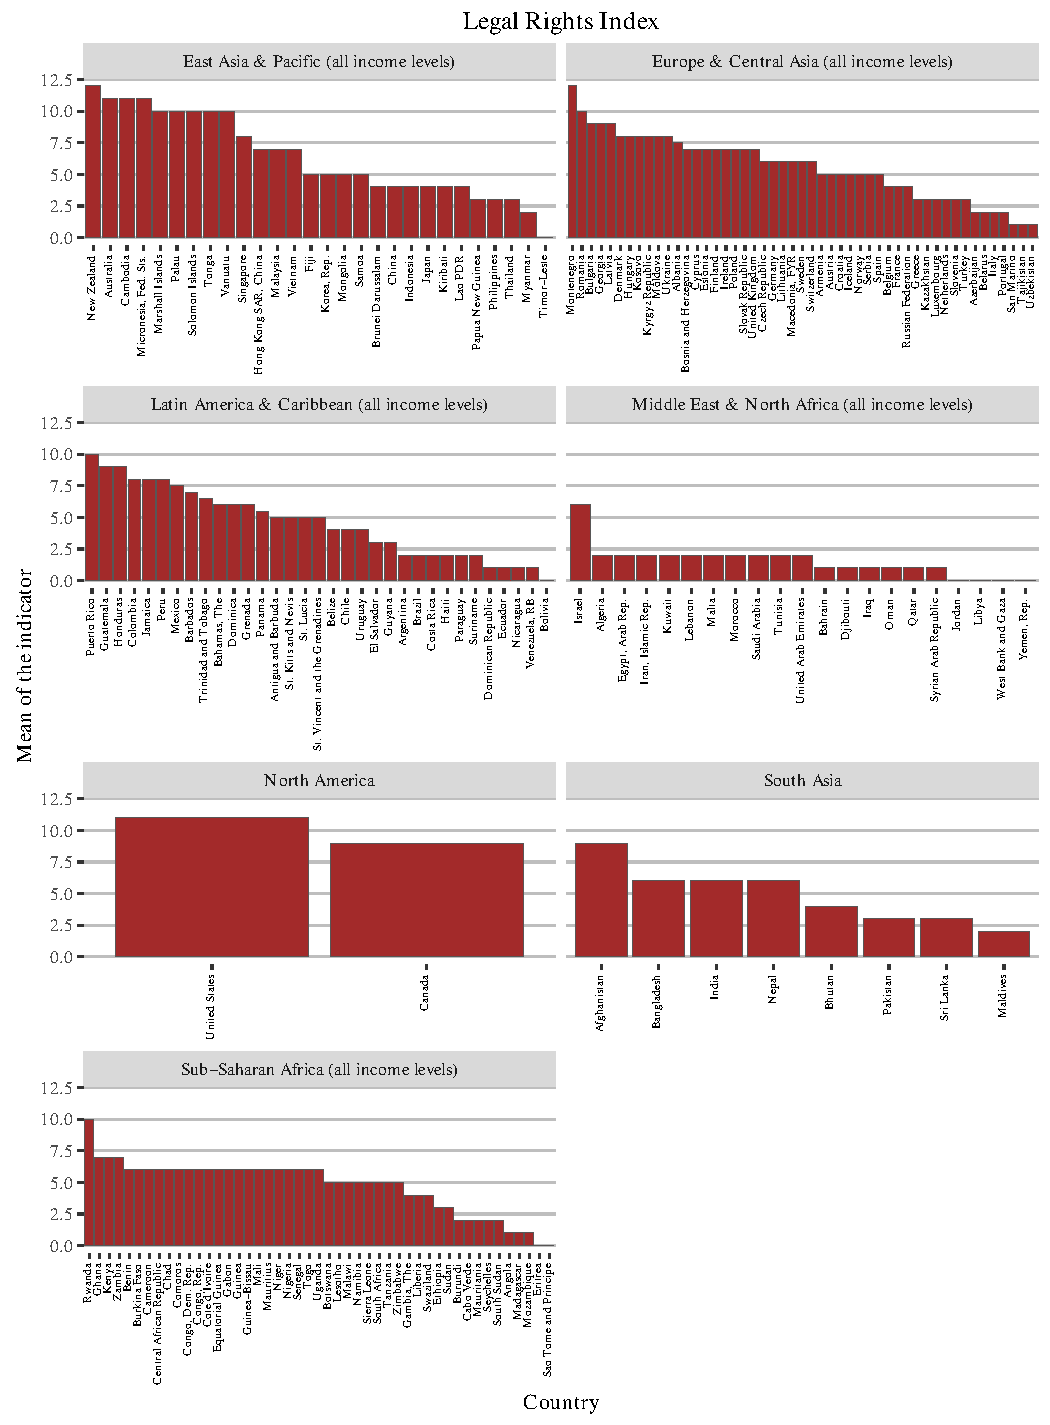
\includegraphics[max height=.9\textheight]{../img/wdi_legal_rights_index.pdf}
\end{center}
\noindent \footnotesize{\textbf{Source:} Own creation and data obtained with package \texttt{WDI}, see the \cite{wb_r}.}
\end{figure}

\begin{figure}[H]
\begin{center}
\caption{WDI: \% of Firms that do not report all sales per Country/Region}
\label{fig_wdi_notsales}
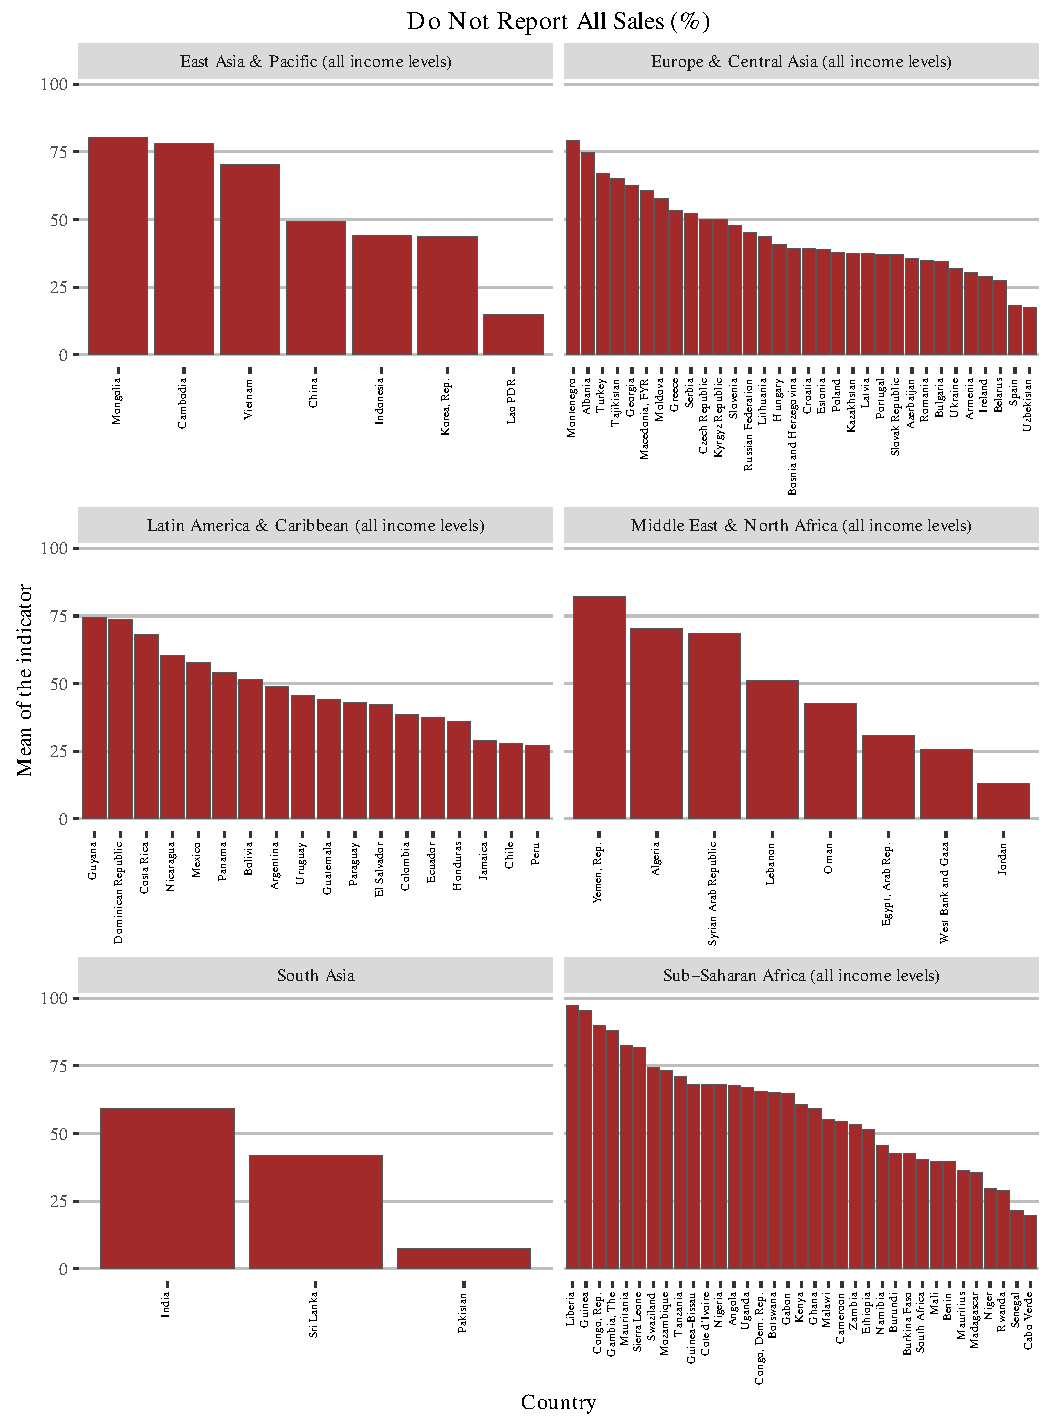
\includegraphics[max height=.9\textheight]{../img/wdi_do_not_report_all_sales_perc.pdf}
\end{center}
\noindent \footnotesize{\textbf{Source:} Own creation and data obtained with package \texttt{WDI}, see the \cite{wb_r}.}
\end{figure}

\begin{figure}[H]
\begin{center}
\caption{WDI: Business disclosure index per Country/Region}
\label{fig_wdi_disclo}
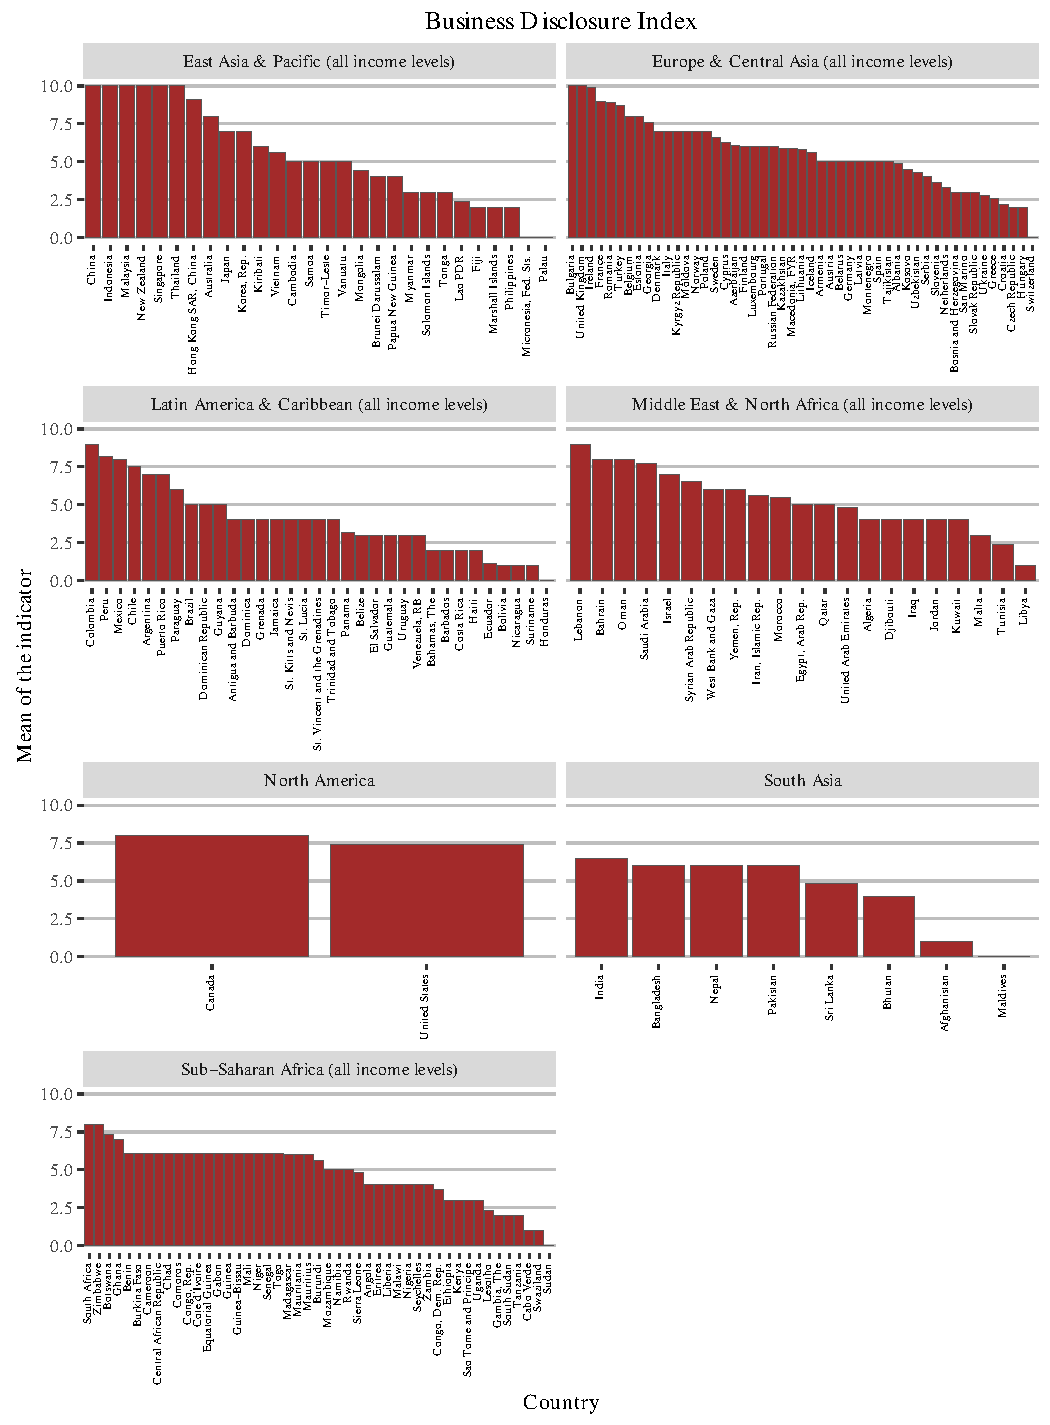
\includegraphics[max height=.9\textheight]{../img/wdi_business_disclosure_index.pdf}
\end{center}
\noindent \footnotesize{\textbf{Source:} Own creation and data obtained with package \texttt{WDI}, see the \cite{wb_r}.}
\end{figure}

\begin{figure}[H]
\begin{center}
\caption{WDI: Gross Domestic Product per Capita per Country/Region}
\label{fig_wdi_gdp}
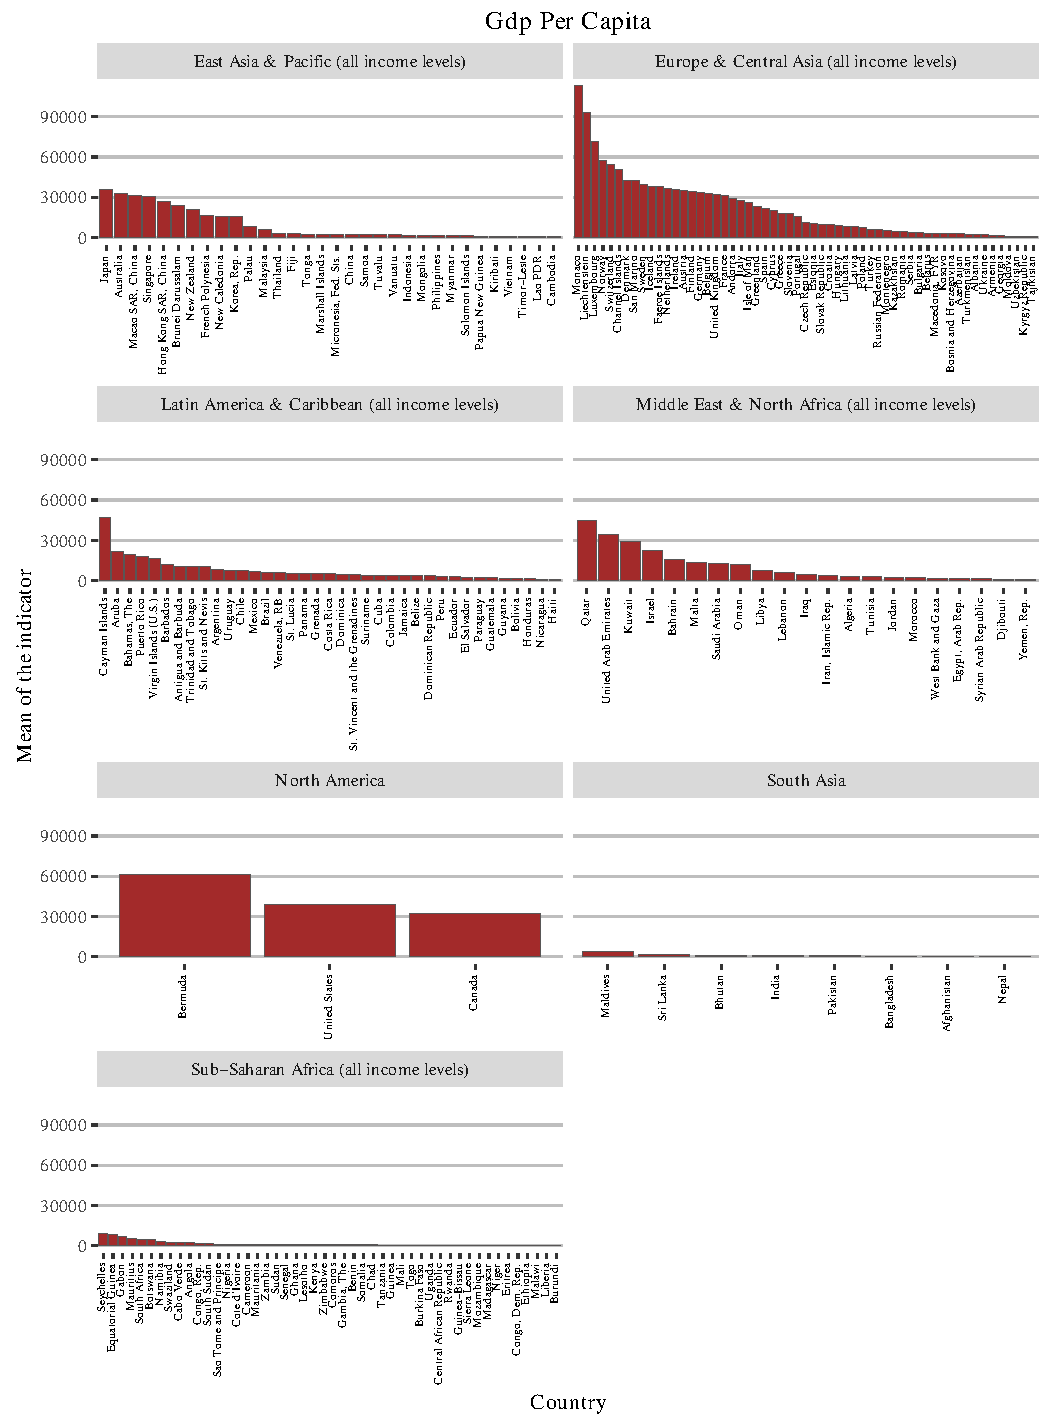
\includegraphics[max height=.9\textheight]{../img/wdi_gdp_per_capita.pdf}
\end{center}
\noindent \footnotesize{\textbf{Source:} Own creation and data obtained with package \texttt{WDI}, see the \cite{wb_r}.}
\end{figure}

\begin{figure}[H]
\begin{center}
\caption{WDI: Gini index of inequality per Country/Region}
\label{fig_wdi_gini}
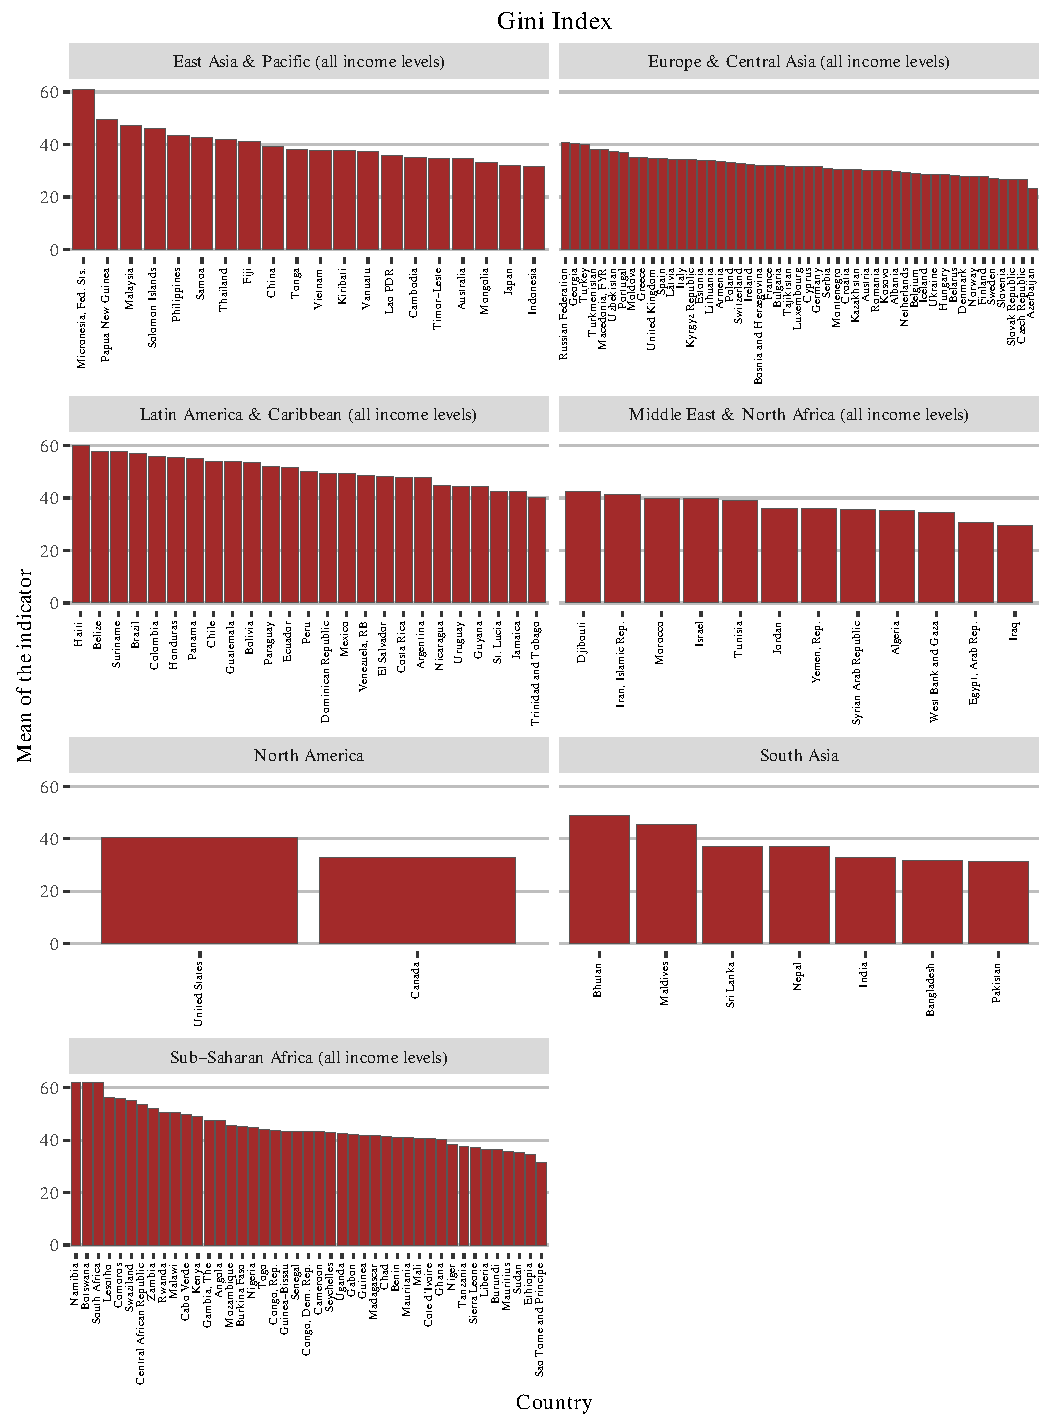
\includegraphics[max height=.9\textheight]{../img/wdi_gini_index.pdf}
\end{center}
\noindent \footnotesize{\textbf{Source:} Own creation and data obtained with package \texttt{WDI}, see the \cite{wb_r}.}
\end{figure}


\begin{figure}[H]
\begin{center}
\caption{WDI: \% of Primary School graduation per Country/Region}
\label{fig_wdi_primary}
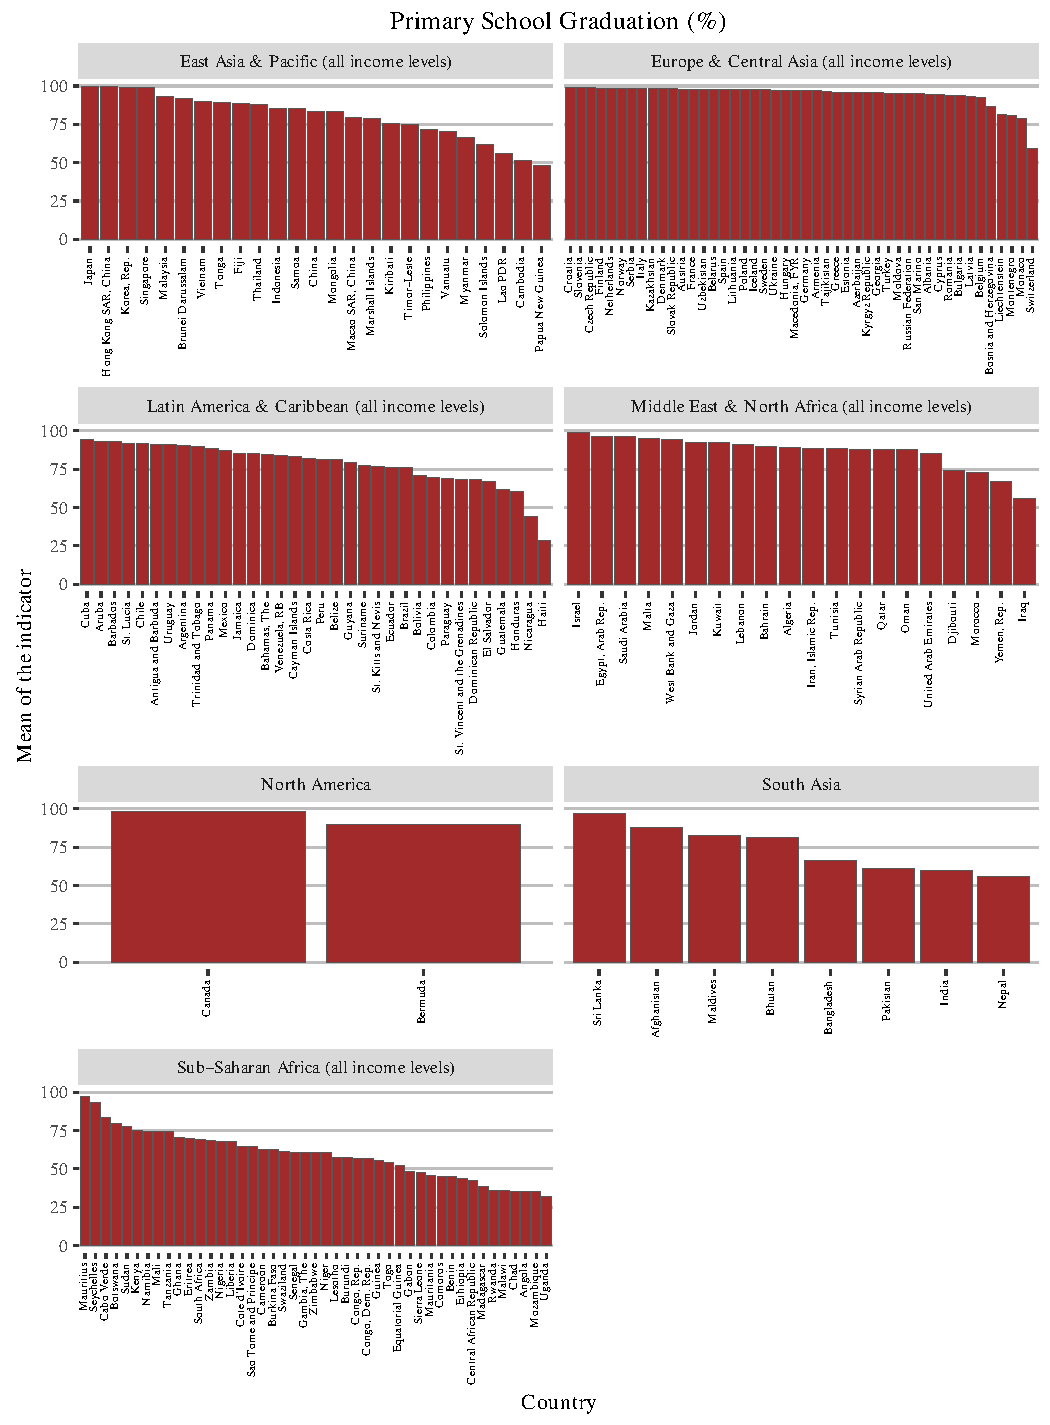
\includegraphics[max height=.9\textheight]{../img/wdi_primary_school_graduation_perc.pdf}
\end{center}
\noindent \footnotesize{\textbf{Source:} Own creation and data obtained with package \texttt{WDI}, see the \cite{wb_r}.}
\end{figure}


\begin{figure}[H]
\begin{center}
\caption{WDI: \% of Unemployment per County/Region}
\label{fig_wdi_unemp}
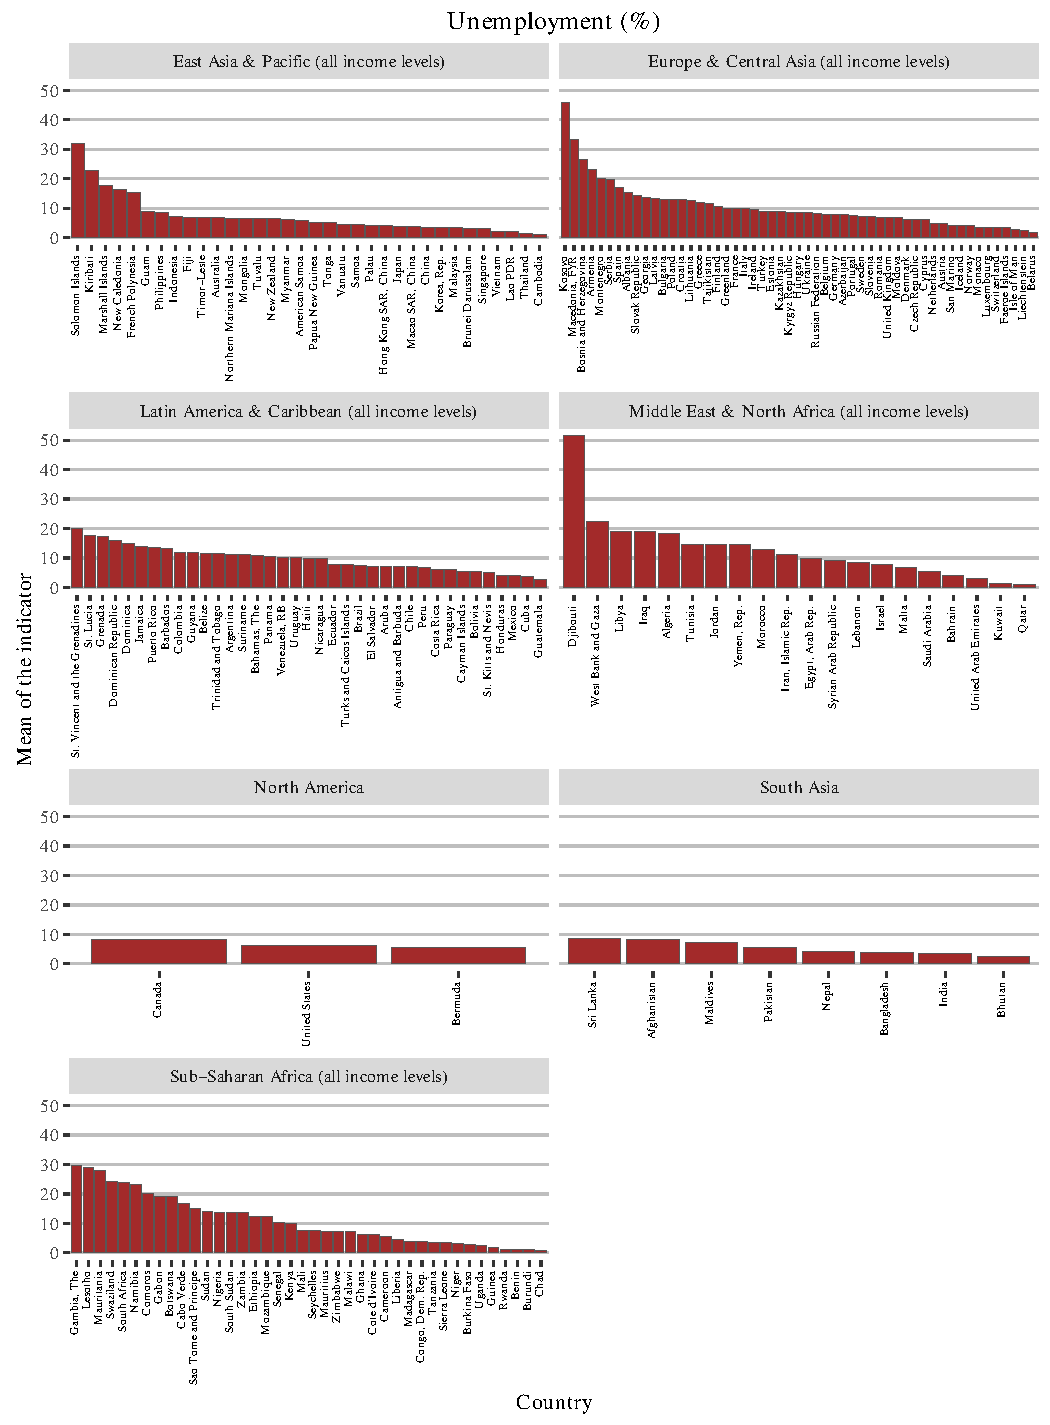
\includegraphics[max height=.9\textheight]{../img/wdi_unemployment_perc.pdf}
\end{center}
\noindent \footnotesize{\textbf{Source:} Own creation and data obtained with package \texttt{WDI}, see the \cite{wb_r}.}
\end{figure}


% !TEX root = A0_thesis_detecting_collusion_corruption_fraud.tex
\chapter{Code}\label{chap_code}

\lstinputlisting[caption=WDI Download code,label=code_wdi]{../code/get_wdi.R}

\newpage
\section{Entity Names disambiguation code}
 
\lstinputlisting[caption=Searches for canonical names,label=code_seaches]{../code/Cluster_Search.py}

\newpage

\lstinputlisting[caption=Cluster canonical names,label=code_cluster_names]{../code/Clustering_Search_Results.py}

\newpage

\lstinputlisting[caption=Models,label=code_models]{../code/svm_latex.py}
\input{X5_wdi.tex}

\printbibheading[heading=bibintoc]
\printbibliography[type=book,heading=subbibintoc,title={Books}]
\printbibliography[type=article,heading=subbibintoc,title={Articles}]
\printbibliography[type=misc,heading=subbibintoc,title={Other references}]


\end{document}
